\documentclass[11pt,a4paper]{article}
% Generated from report.md by report/md_to_latex.py. Edit report.md and regenerate, or edit this file directly
% once the team switches to LaTeX as the source.
\usepackage[utf8]{inputenc}
\usepackage[T1]{fontenc}
\usepackage{lmodern}
\usepackage[margin=18mm]{geometry}
\usepackage{graphicx}
\usepackage{booktabs}
\usepackage{array}
\usepackage{xltabular}
\usepackage{caption}
\usepackage{enumitem}
\usepackage{xcolor}
\usepackage{newunicodechar}
\usepackage{microtype}
\usepackage[hidelinks]{hyperref}
\usepackage{xurl}

\graphicspath{{../figures/}{figures/}}
\setlist[itemize]{itemsep=2pt, topsep=4pt, leftmargin=*}
\captionsetup{font=small, labelfont=bf}
\renewcommand{\arraystretch}{1.15}
\setlength{\parindent}{0pt}
\setlength{\parskip}{5pt}

% Characters used in the text that pdfLaTeX does not map by default
\newunicodechar{−}{\ensuremath{-}}
\newunicodechar{≤}{\ensuremath{\le}}
\newunicodechar{≥}{\ensuremath{\ge}}
\newunicodechar{×}{\ensuremath{\times}}
\newunicodechar{·}{\textperiodcentered}
\newunicodechar{²}{\textsuperscript{2}}
\newunicodechar{±}{\ensuremath{\pm}}
\newunicodechar{ρ}{\ensuremath{\rho}}
\newunicodechar{Δ}{\ensuremath{\Delta}}
\newunicodechar{→}{\ensuremath{\rightarrow}}
\newunicodechar{≈}{\ensuremath{\approx}}

\title{Formula 1 Podium Prediction\\[4pt]\large CSEN 903 · Milestone 1 · Analytical Report}
\author{Kevin Sherif (58-0484) \and Zeyad Sameh (58-3364) \and Marina Medhat (58-5270) \and Abdelrahman Mahmoud (58-2414)}
\date{18 October 2026}
\begin{document}
\maketitle
\begin{center}\small
\textbf{Notebook (Kaggle):} KAGGLE NOTEBOOK LINK \\ \textbf{Repository:} \url{https://github.com/Abdel-RahmanIII/Formula-1}
\end{center}
\section{Summary}

\textbf{Task.} Predict whether a driver finishes on the podium (top three) of a Formula 1 race, using only information available after qualifying and before the start. The data are the 14 relational tables of the Ergast Formula 1 dataset, 1950–2024.

\textbf{What was built.} One notebook that audits and cleans the raw tables, answers three data-engineering questions, builds a table of 21 pre-race features with one row per driver per race, trains and compares five models, measures what each feature group contributes, explains the selected model, and wraps it in an inference function.

\textbf{Main results}

\begin{itemize}
\item \textbf{The modeling table has 24,482 rows}, one per \texttt{(raceId, driverId)}, after removing the Indianapolis 500 races, 1,715 non-starters and 157 rows of cars that two drivers shared from the 26,759 raw rows. Each removal is backed by the instructors' rulings or by retraining with the rows kept.
\item \textbf{All four learned models beat the baseline, and none beats the others.} On the unseen test seasons (2022–2024) PR-AUC is 0.707 to 0.720 for the learned models, against 0.647 for a rule that predicts the first three grid slots. The pre-race features are worth about 0.06 PR-AUC; model complexity adds nothing measurable.
\item \textbf{The model is mostly a model of the starting grid.} Starting position (grid and qualifying) carries most of the signal, the recent results of the driver and team add a smaller amount (clear on validation, weaker on the test seasons), and race context adds nothing.
\item \textbf{No data leakage.} Every history feature uses only earlier races. Two tests in the notebook verify this, and the inference function reproduces the features from pre-race information alone.
\item \textbf{The limit is the race itself.} The clearest errors are results decided by in-race events, which no pre-race input contains.
\end{itemize}

The split, used throughout: \textbf{train} on seasons up to 2019, \textbf{validate} on 2020–2021, \textbf{test} on 2022–2024. A split by time is used because a random split would train on later seasons than it tests on, and would leak era-specific knowledge about which teams are fast.

{\small
\begin{xltabular}{\linewidth}{>{\raggedright\arraybackslash}Xrrrr}
\toprule
\textbf{Split} & \textbf{Rows} & \textbf{Races} & \textbf{Podiums} & \textbf{Podium rate} \\
\midrule
\endhead
Train (≤ 2019) & 22,355 & 1,007 & 3,004 & 13.44\% \\
Validation (2020–2021) & 775 & 39 & 117 & 15.10\% \\
Test (2022–2024) & 1,352 & 68 & 204 & 15.09\% \\
\bottomrule
\end{xltabular}
}

Every judgment call is recorded with its evidence in the decision log of the repository (DEC-001 to DEC-039); the identifiers are cited below.

\section{Data Audit and Cleaning}

\subsection{Audit of the raw tables}

\begin{itemize}
\item \textbf{Size.} 14 tables, 701,433 rows. \texttt{results} has 26,759 rows over 1,125 races. \texttt{lap\_\allowbreak{}times} is 84\% of all rows and is recorded during the race, so it is forbidden as a feature.
\item \textbf{Primary keys.} All 16 keys checked (single and composite) are unique and non-null, with one known exception handled in cleaning: \texttt{results} has repeated \texttt{(raceId, driverId)} pairs.
\item \textbf{Foreign keys.} All 22 foreign keys were reconciled with anti-joins. None has an orphan row.
\item \textbf{Sentinels.} Missing values are written as the text \texttt{\textbackslash{}N}. They are read as missing at load time.
\item \textbf{Raw tables are never modified.} All cleaning works on copies, and the notebook asserts at the end that the raw tables equal a fresh load.
\end{itemize}

Two findings from the ''before'' plots shaped later decisions:

\begin{itemize}
\item \textbf{Qualifying coverage drifts.} There is no qualifying data before 1994, coverage is between 6\% and 59\% of result rows in 1996–2002, and it is complete only from 2003.
\item \textbf{The podium rate depends on field size.} It is 12.69\% over all raw rows, falls to 7.74\% in 1989 when entry lists were longest, and is near 15\% in the modern 20-car era.
\end{itemize}

\begin{figure}[htbp]
\centering
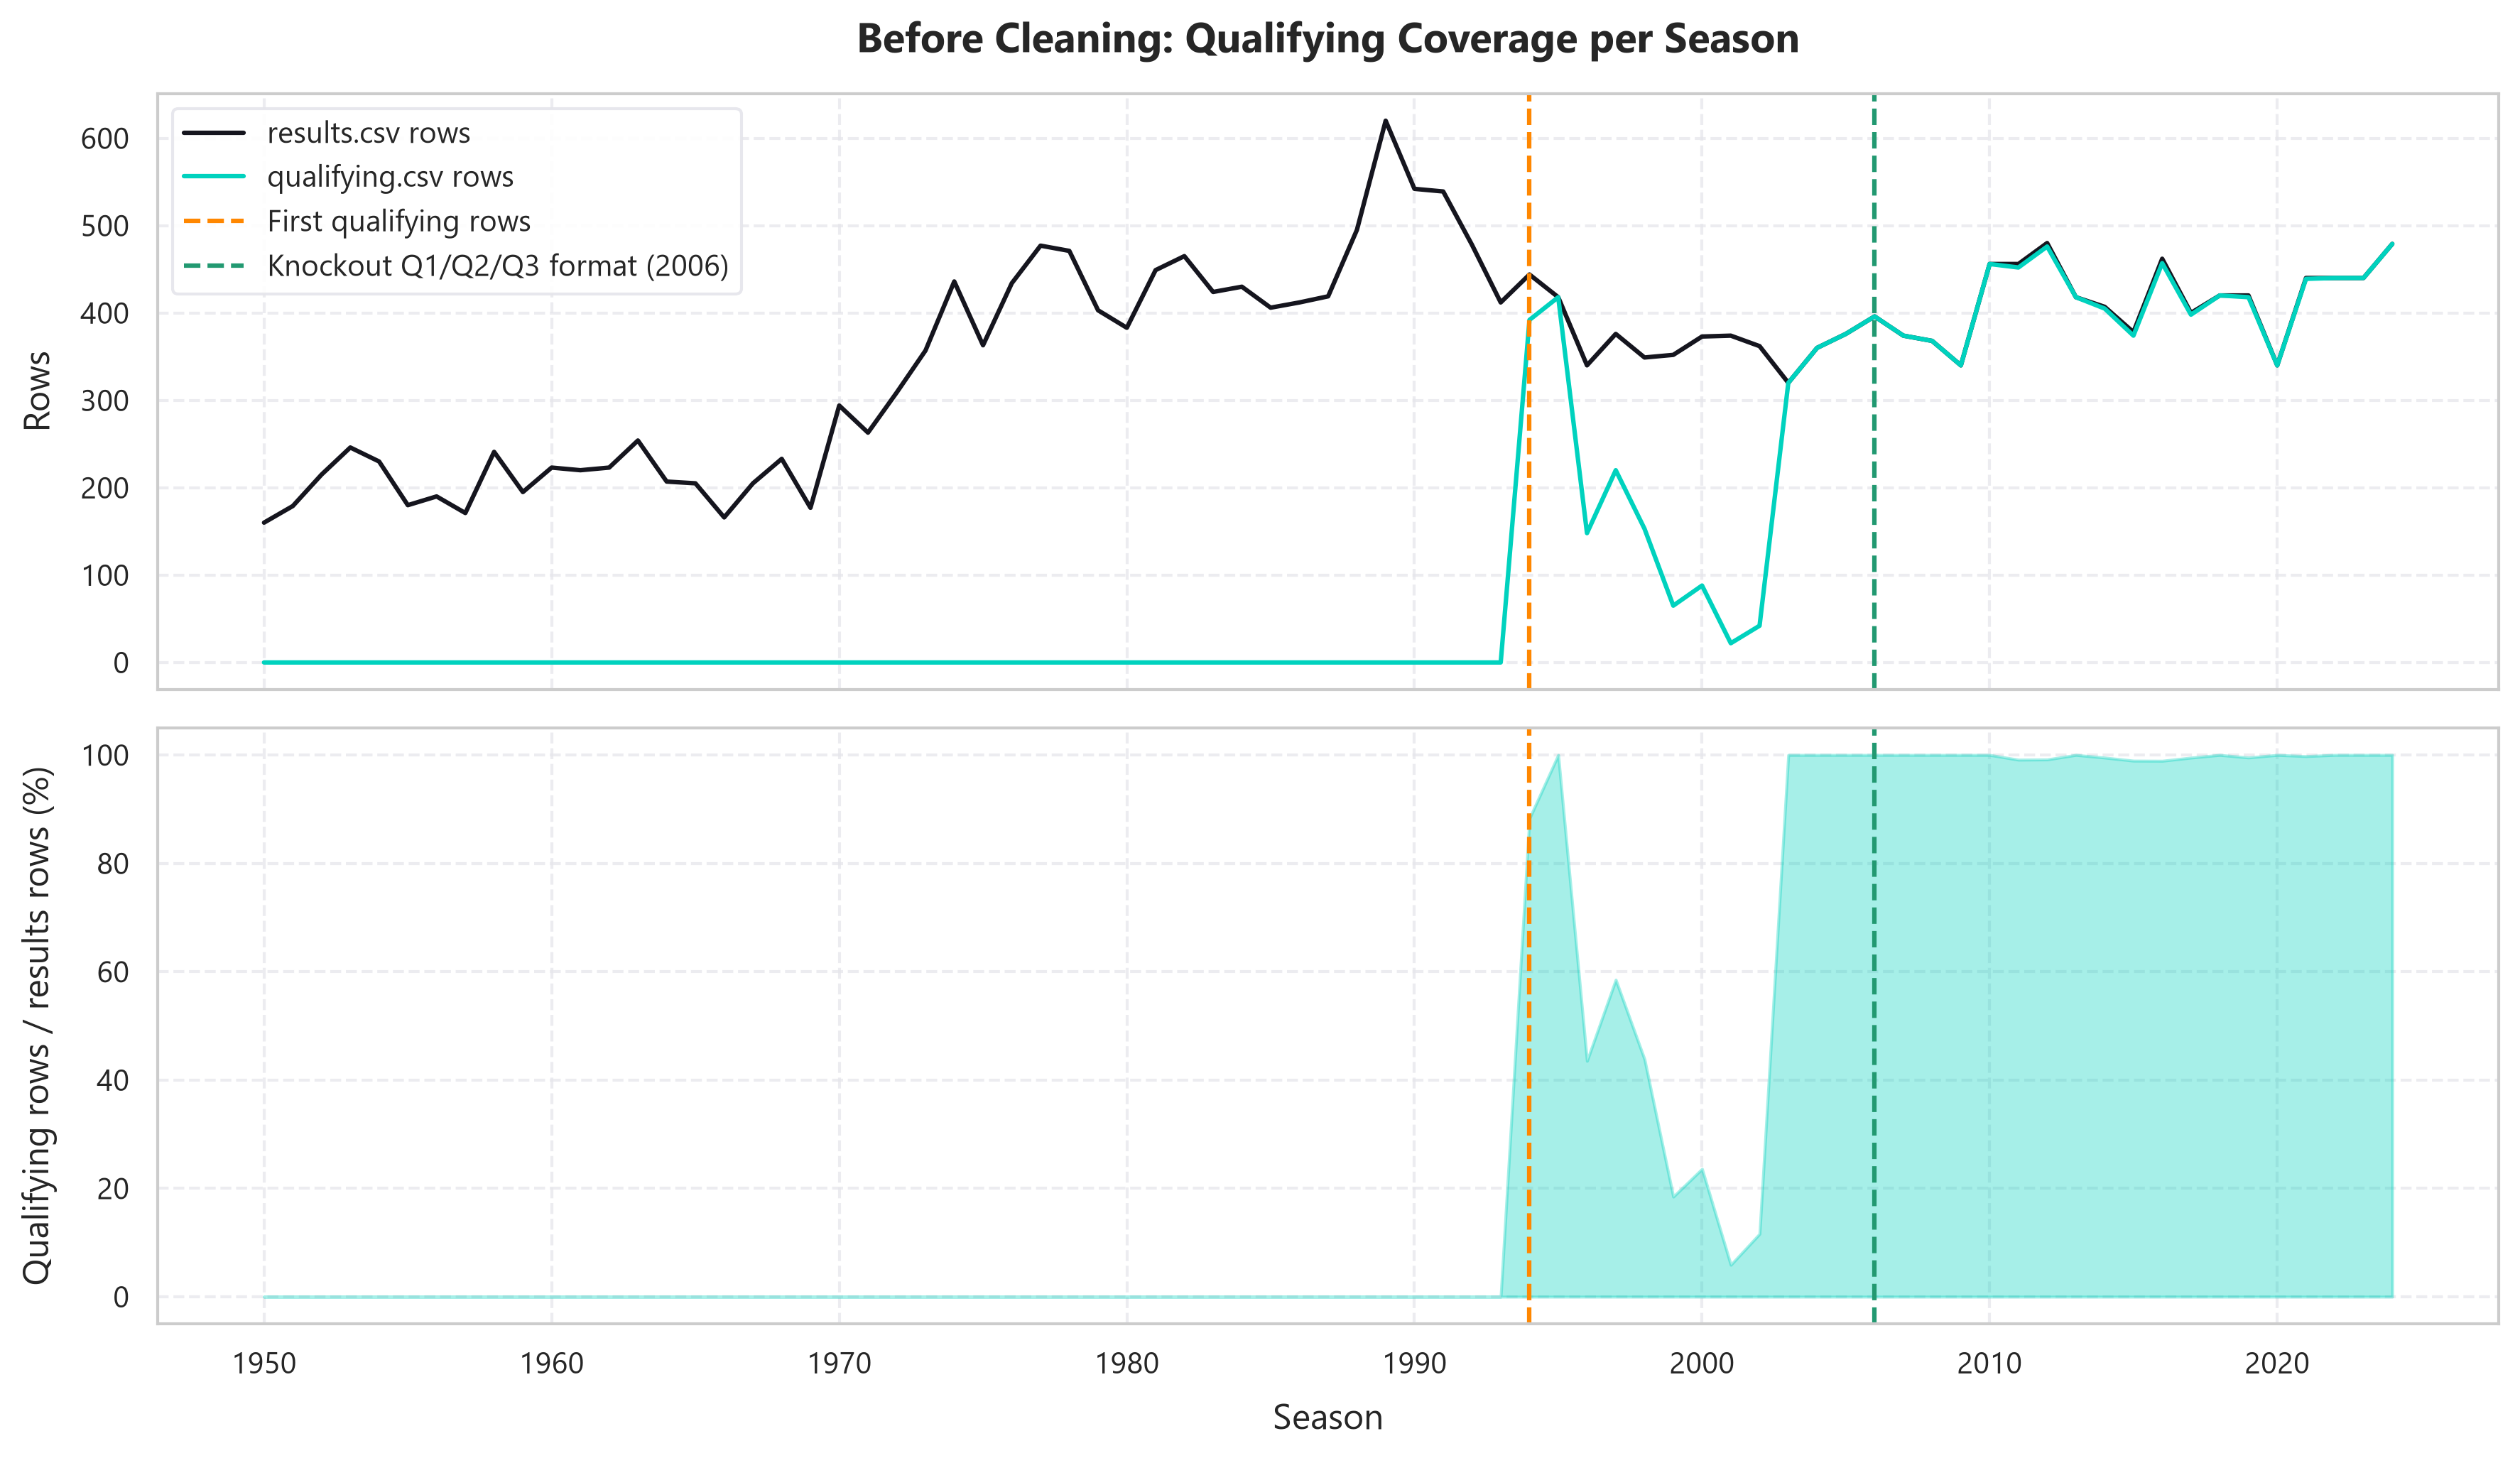
\includegraphics[width=\linewidth,height=0.42\textheight,keepaspectratio]{before_eda_qualifying_coverage}
\caption{Rows per season in \texttt{results} and \texttt{qualifying} (top) and qualifying rows as a share of result rows (bottom). Qualifying is complete only from 2003.}
\end{figure}

\subsection{Cleaning steps}

{\small
\begin{xltabular}{\linewidth}{>{\raggedright\arraybackslash}X>{\raggedright\arraybackslash}Xrr}
\toprule
\textbf{Step} & \textbf{Rule} & \textbf{Rows removed} & \textbf{Rows left} \\
\midrule
\endhead
Raw \texttt{results} &  &  & 26,759 \\
Scope (DEC-003) & Drop the Indianapolis 500 races of 1950–1960: run to different rules, on an oval, with a different field & 405 & 26,354 \\
Non-starters (DEC-009) & Drop a row when the driver completed zero laps \textbf{and} is labelled as not qualified or withdrawn, or had no grid slot & 1,715 & 24,639 \\
Shared drives (DEC-034) & Remove every row of a car listed under two drivers (same team, grid slot and classification); a driver who also drove a car of their own keeps that row & 157 & 24,482 \\
\bottomrule
\end{xltabular}
}

\begin{itemize}
\item \textbf{Semantic typing.} Dates are converted to datetime. Qualifying times and pit-stop durations such as \texttt{"1:24.312"} are converted to seconds (84.312). The count of missing values is the same before and after conversion, so no time was lost in parsing.
\item \textbf{Why ''zero laps'' is part of the non-starter rule.} The label alone is unreliable: 1,724 rows carry a non-starter label, but 24 of them completed racing laps. No podium finisher is removed.
\item \textbf{Evidence for the removals.} The instructors allow removing \texttt{F} (failed to qualify) because it is known before the race, and require an experiment for \texttt{W} (withdrawn) and evidence for any excluded data. Both are tested by retraining with the rows kept (Section 7): the Indianapolis 500 makes no difference, and the withdrawn entries make the model worse, so both removals stand.
\item \textbf{Shared drives.} Until the mid-1960s a driver could take over a teammate's car during a race. The data then lists the shared car under both drivers with the same grid slot and classification, without saying who started it. Keeping either row would pair one driver's starting slot with another driver's result, which the instructors ruled to be data leakage. Every row of a shared car is therefore removed: 155 rows in 40 races of 1950–1964, plus one driver left with two cars of their own. 43 drivers keep a car they drove alone. An earlier rule kept each driver's best-classified row; 59 of the 61 rows it kept were shared cars, so it was replaced (DEC-034).
\item \textbf{Pit-lane starts (DEC-010).} The 72 remaining rows with \texttt{grid = 0} are real pit-lane starts. Left as 0, a model would read them as better than pole. They get \texttt{pit\_\allowbreak{}start = 1} and a grid slot one place behind the last car.
\end{itemize}

\subsection{Effect of cleaning}

\begin{itemize}
\item \textbf{8.5\% of raw rows are removed}, most of them non-starters from the crowded entry lists of the 1970s to 1990s. The largest ''field'' falls from 55 entries to 34 starters.
\item \textbf{The podium rate rises from 12.69\% to 13.58\%.} From the mid-1990s the before and after lines coincide, so cleaning does not distort the seasons used for validation and testing.
\item \textbf{No race has more than three podium rows.} Two races keep one and 13 keep two, because their other podium cars were shared and removed.
\end{itemize}

\begin{figure}[htbp]
\centering
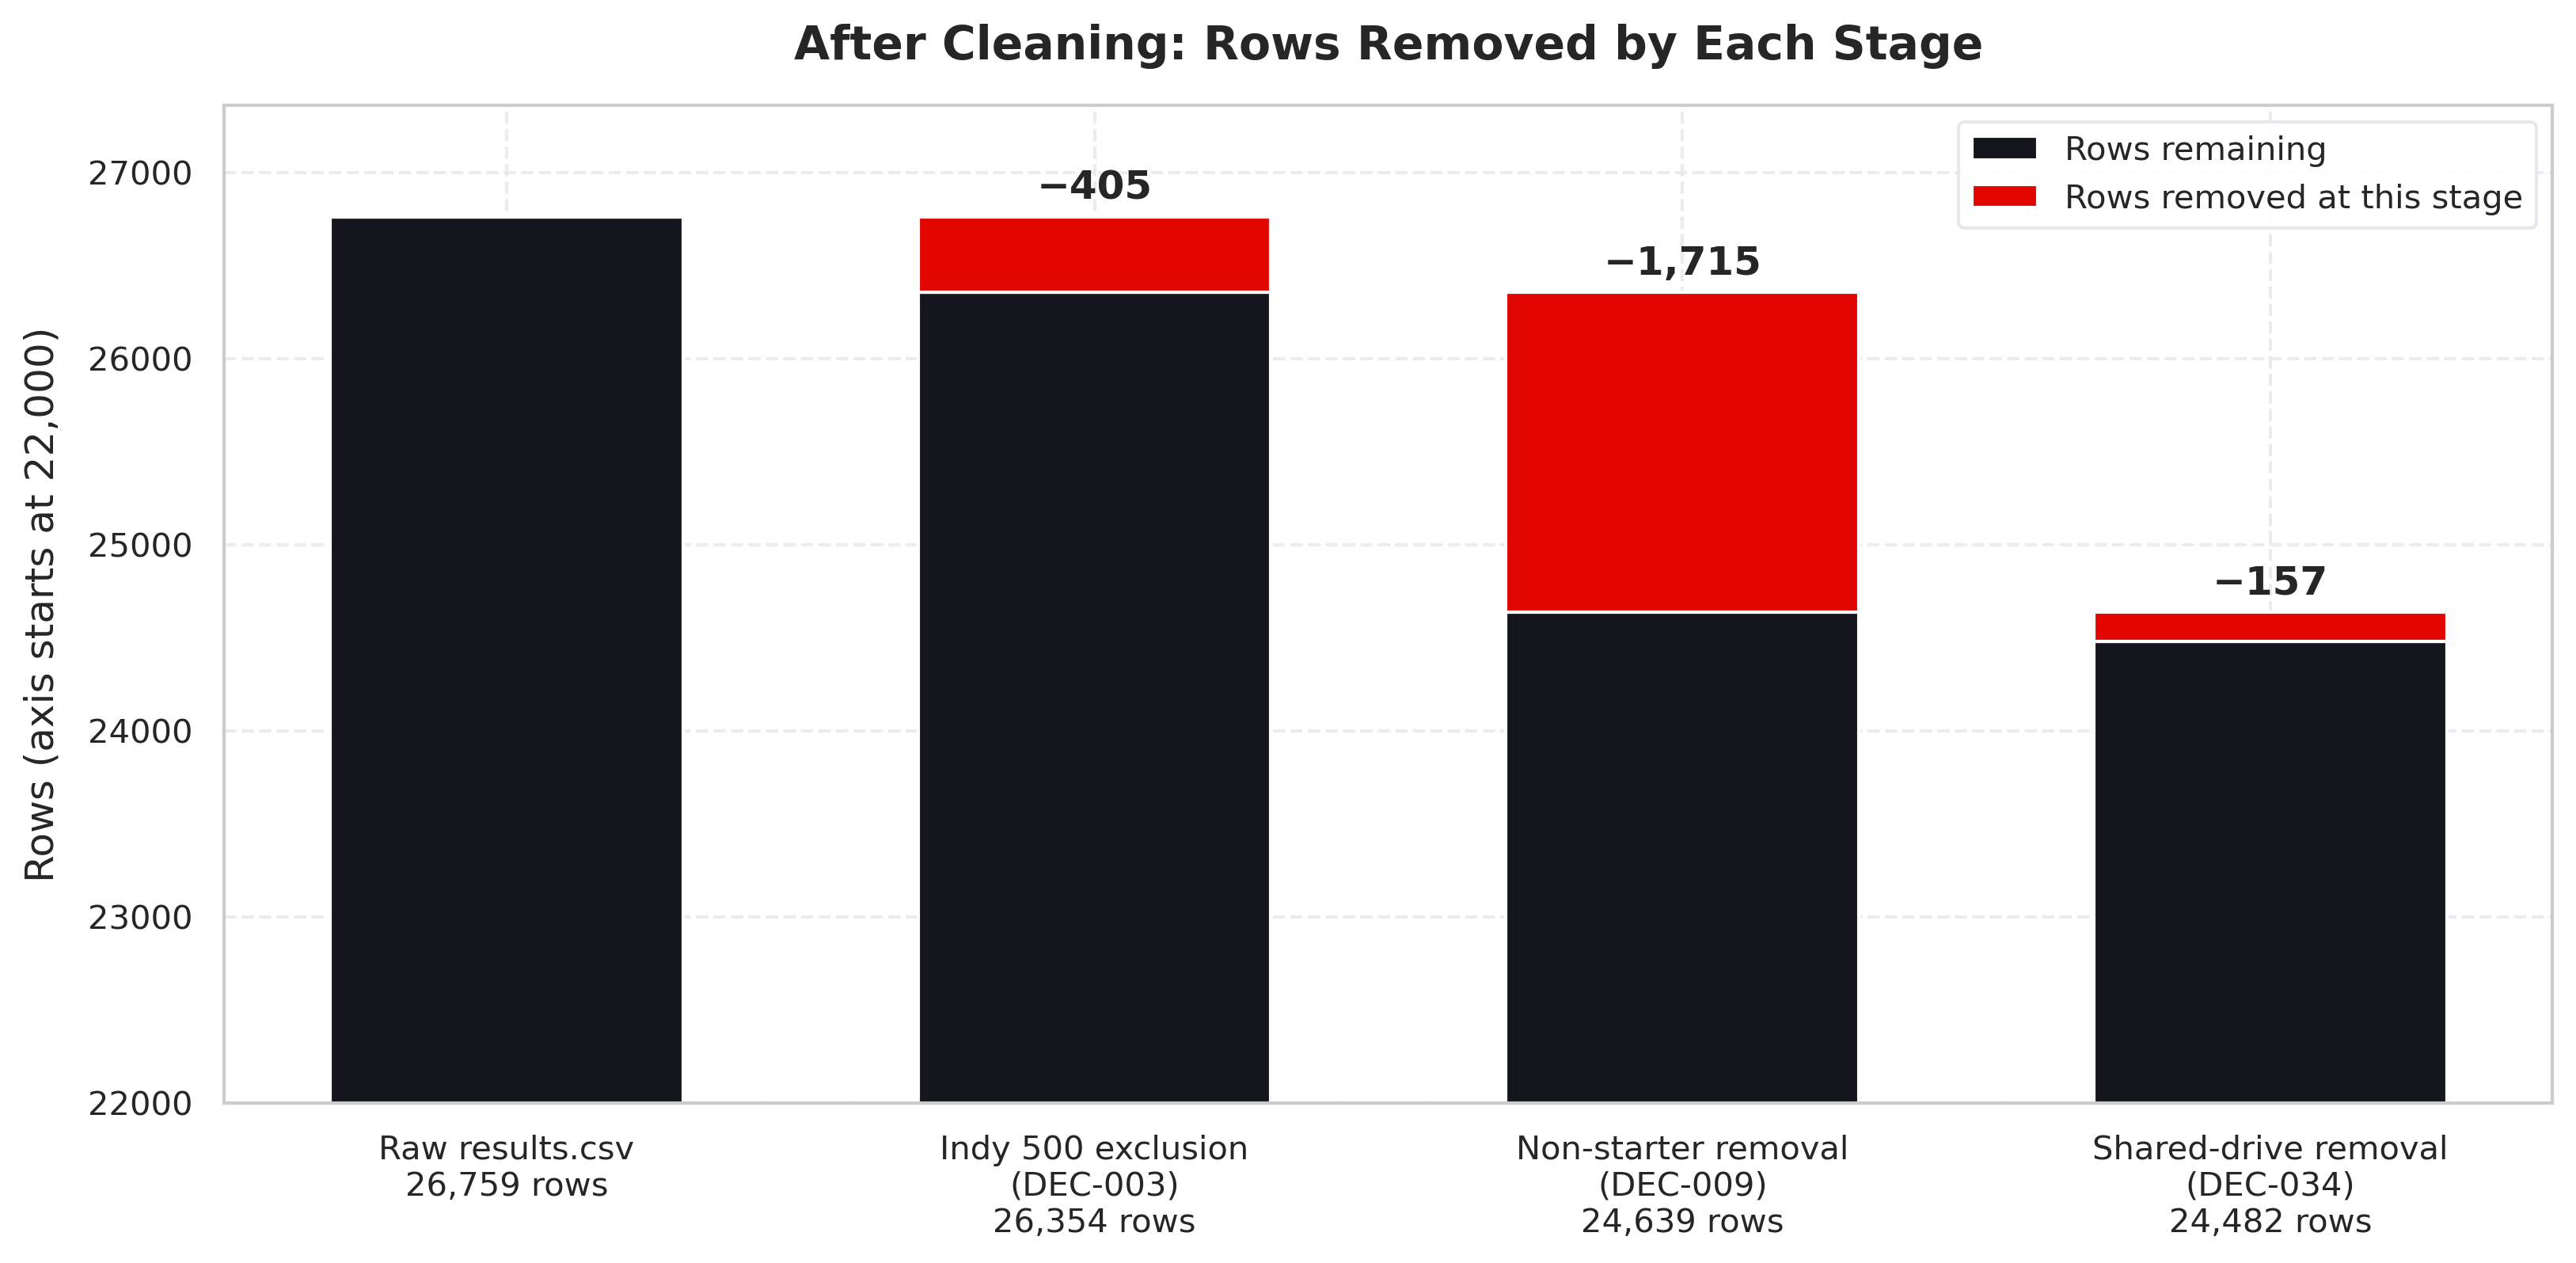
\includegraphics[width=\linewidth,height=0.42\textheight,keepaspectratio]{after_eda_row_count_waterfall}
\caption{Rows remaining after each cleaning stage (dark) and rows removed by that stage (red). The axis starts at 22,000.}
\end{figure}

\begin{figure}[htbp]
\centering
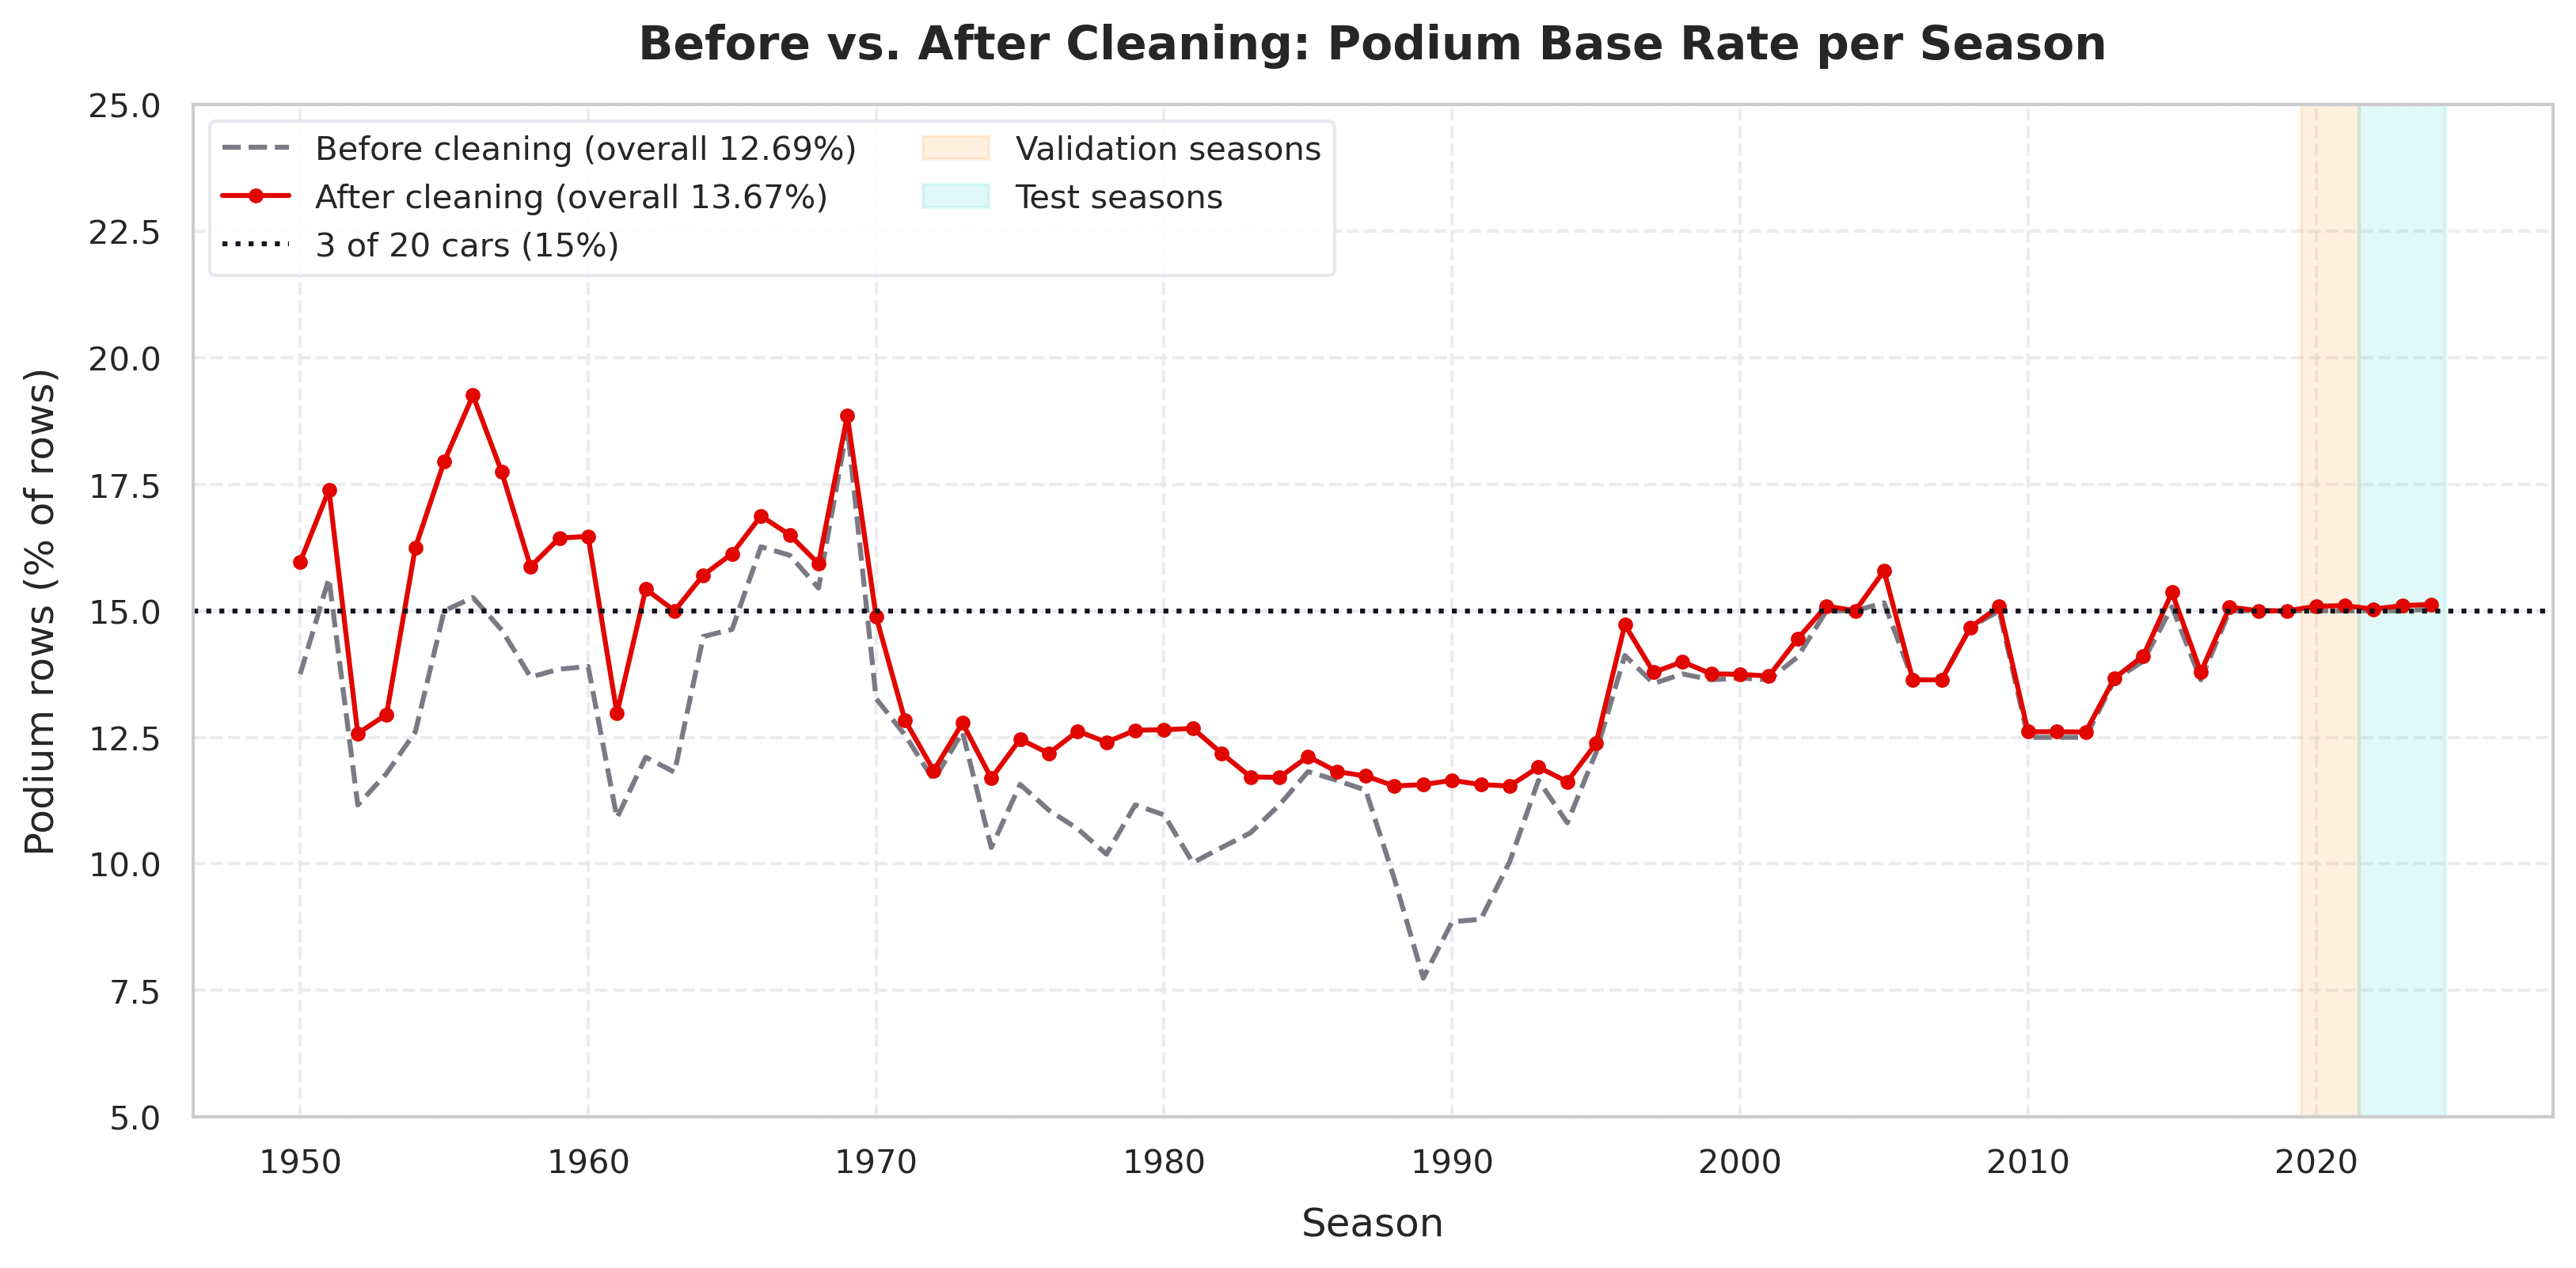
\includegraphics[width=\linewidth,height=0.42\textheight,keepaspectratio]{after_eda_podium_base_rate}
\caption{Podium rate per season before (grey, dashed) and after (red) cleaning. The shaded bands are the validation and test seasons.}
\end{figure}

\section{Data-Engineering Questions}

The three questions are descriptive analyses. Outcome columns such as \texttt{podium} and \texttt{status} are what is being measured; they are never model features. Every grouping variable is known before the race.

\subsection{Q1: Which circuits convert a front-row start into a podium, and did the ranking change after 2014?}

\textbf{Answer. Front-row starts convert far more often in the hybrid era, and the circuit ranking is not preserved.}

\begin{itemize}
\item \textbf{Definition (DEC-035).} A front-row start is a start from grid slot 1 or 2. Only the grid is used, as the instructors specified: the brief's note on qualifying is a reminder that penalties make the two differ, not a request for a second rate. Because the grid is recorded for every race, every season is used: 1950–2013 against 2014–2024.
\item \textbf{Overall.} A front-row start ended on the podium 56.3\% of the time in 1950–2013 (991 of 1,759) and 76.2\% in 2014–2024 (345 of 453). The rate rose at 14 of the 16 ranked circuits.
\item \textbf{Top circuits, 2014–2024.} Monaco (89.5\%), Suzuka (88.9\%), Yas Marina (86.4\%). The Hungaroring is last (59.1\%).
\item \textbf{Top circuits, 1950–2013.} Suzuka (70.0\%), the Hungaroring (67.9\%), then Barcelona and Bahrain (both 66.7\%).
\item \textbf{Ranking.} The Spearman correlation between the two eras is −0.08 (p = 0.76): a circuit's rank before 2014 says nothing about its rank after. Monaco climbs from 15th to 1st; the Hungaroring falls from 2nd to 16th.
\item \textbf{Sensitivity.} With a pre-hybrid window as long as the hybrid one (2003–2013), the rise is smaller (67.0\% to 76.2\%) and the ranking is still only loosely kept (ρ = 0.36). Both windows give the same answer.
\item \textbf{How far to trust it.} In 2014–2024 each circuit has 14 to 26 front-row starts, so one race moves a rate by 4 to 7 points. The rise in the overall level is solid; individual rank changes are mostly within that noise.
\end{itemize}

\begin{figure}[htbp]
\centering
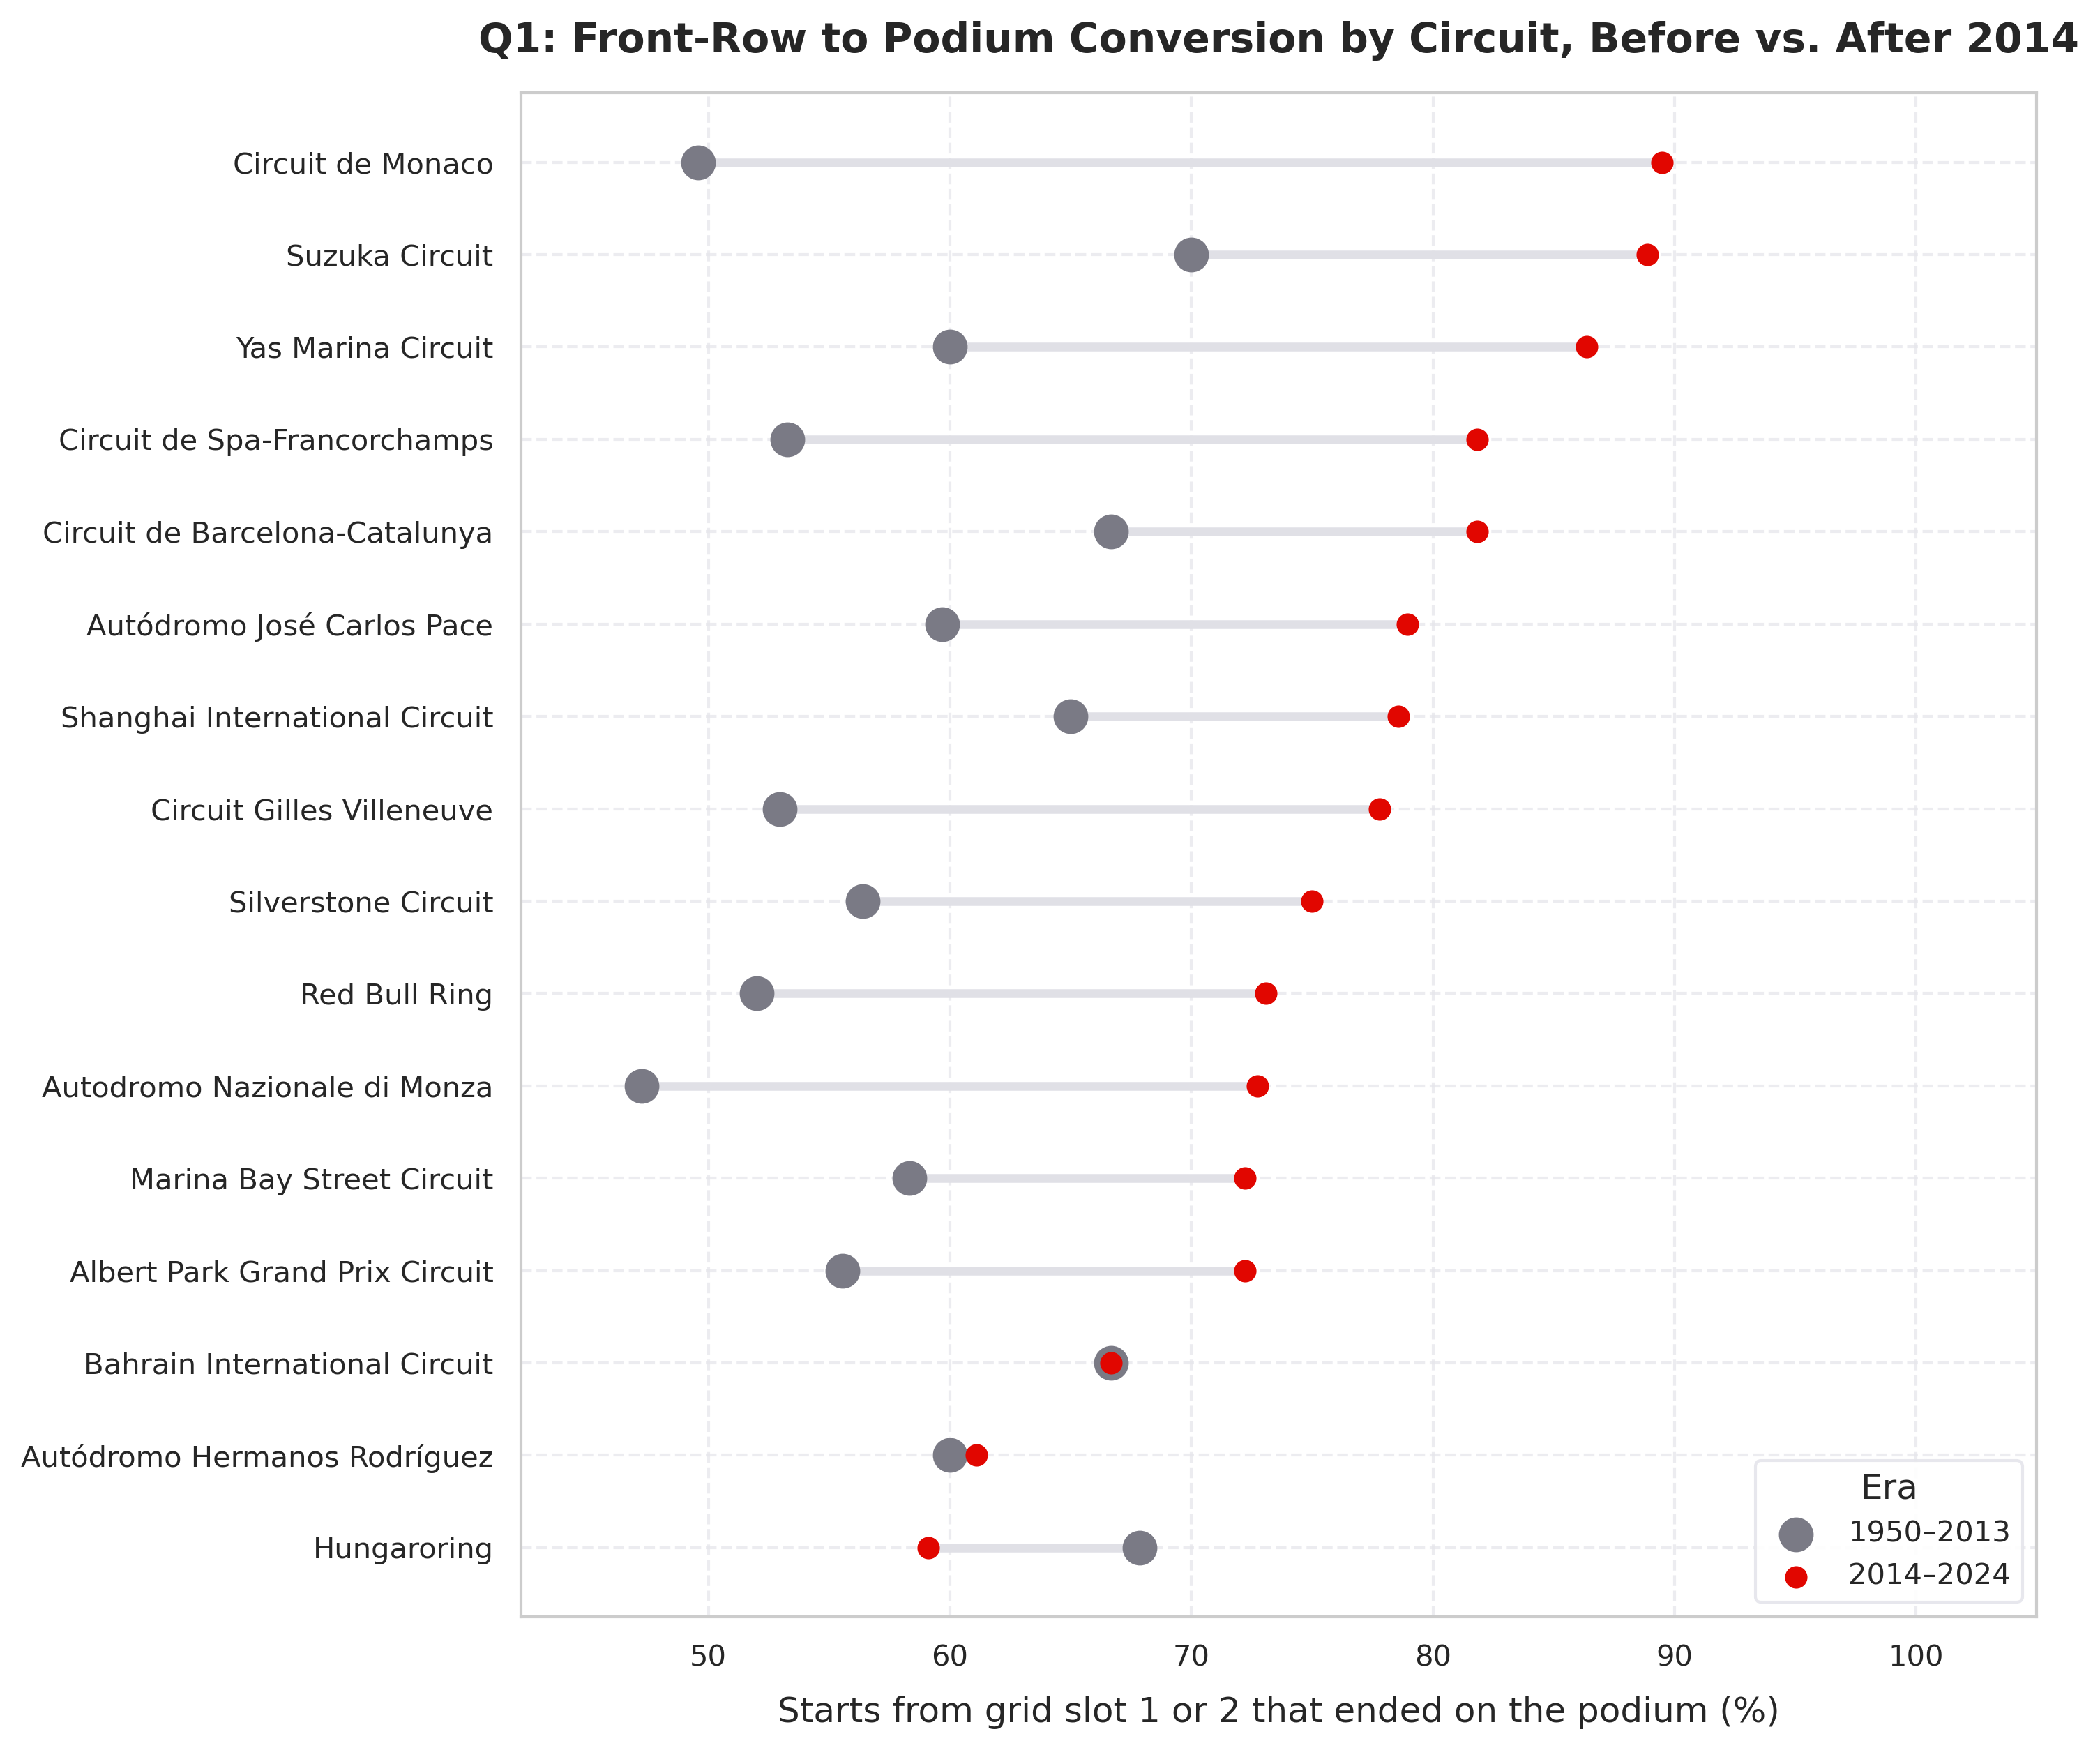
\includegraphics[width=\linewidth,height=0.42\textheight,keepaspectratio]{de_q1_front_row_conversion}
\caption{Podium rate of starters from grid slot 1 or 2 per circuit, 1950–2013 (grey) and 2014–2024 (red). Circuits with at least 10 front-row starts in each era.}
\end{figure}

{\small
\begin{xltabular}{\linewidth}{>{\raggedright\arraybackslash}X>{\raggedright\arraybackslash}X}
\toprule
\textbf{Joins} & \texttt{results} + \texttt{races} + \texttt{circuits}; no qualifying data is needed \\
\textbf{Grain} & One row per driver per race; rates aggregated per circuit and era \\
\textbf{Missing values} & None: every start has a grid slot. 17 races have fewer than two front-row starts, because a front-row car did not start or was a shared car. Circuits with fewer than 10 front-row starts in either era are not ranked \\
\textbf{Pre-race cutoff} & The grid slot is fixed before the start. \texttt{podium} is used only as the outcome \\
\bottomrule
\end{xltabular}
}

\subsection{Q2: Do drivers reach the podium more often at home, after controlling for starting position?}

\textbf{Answer. No. Once starting position is held fixed, there is no detectable home advantage.}

\begin{itemize}
\item \textbf{Before controlling for grid} the home rate is lower: 11.57\% at home against 13.75\% away. That gap comes from where home drivers start: 11.9\% of home starts are from the first three grid slots, against 13.7\% of away starts.
\item \textbf{Within grid buckets} (1, 2–3, 4–6, 7–10, 11+) the difference goes both ways, from −4.3 points on pole to +2.4 points from slots 2–3, and every pair of intervals overlaps.
\item \textbf{Significance.} The Cochran–Mantel–Haenszel pooled odds ratio for a home race is 0.91 (95\% interval 0.76 to 1.08, p = 0.31). A logistic regression of podium on home race and grid bucket agrees: 0.91 (0.75 to 1.11, p = 0.35).
\item \textbf{Robustness.} The result holds with the exact grid slot instead of buckets (0.92), with only drivers who ever had a home race (0.90), and with the decade added (0.91).
\item \textbf{What it rules out.} A large home advantage: at most about 8\% higher odds. It does not rule out a home effect on qualifying itself, because conditioning on grid removes that channel by design.
\end{itemize}

\begin{figure}[htbp]
\centering
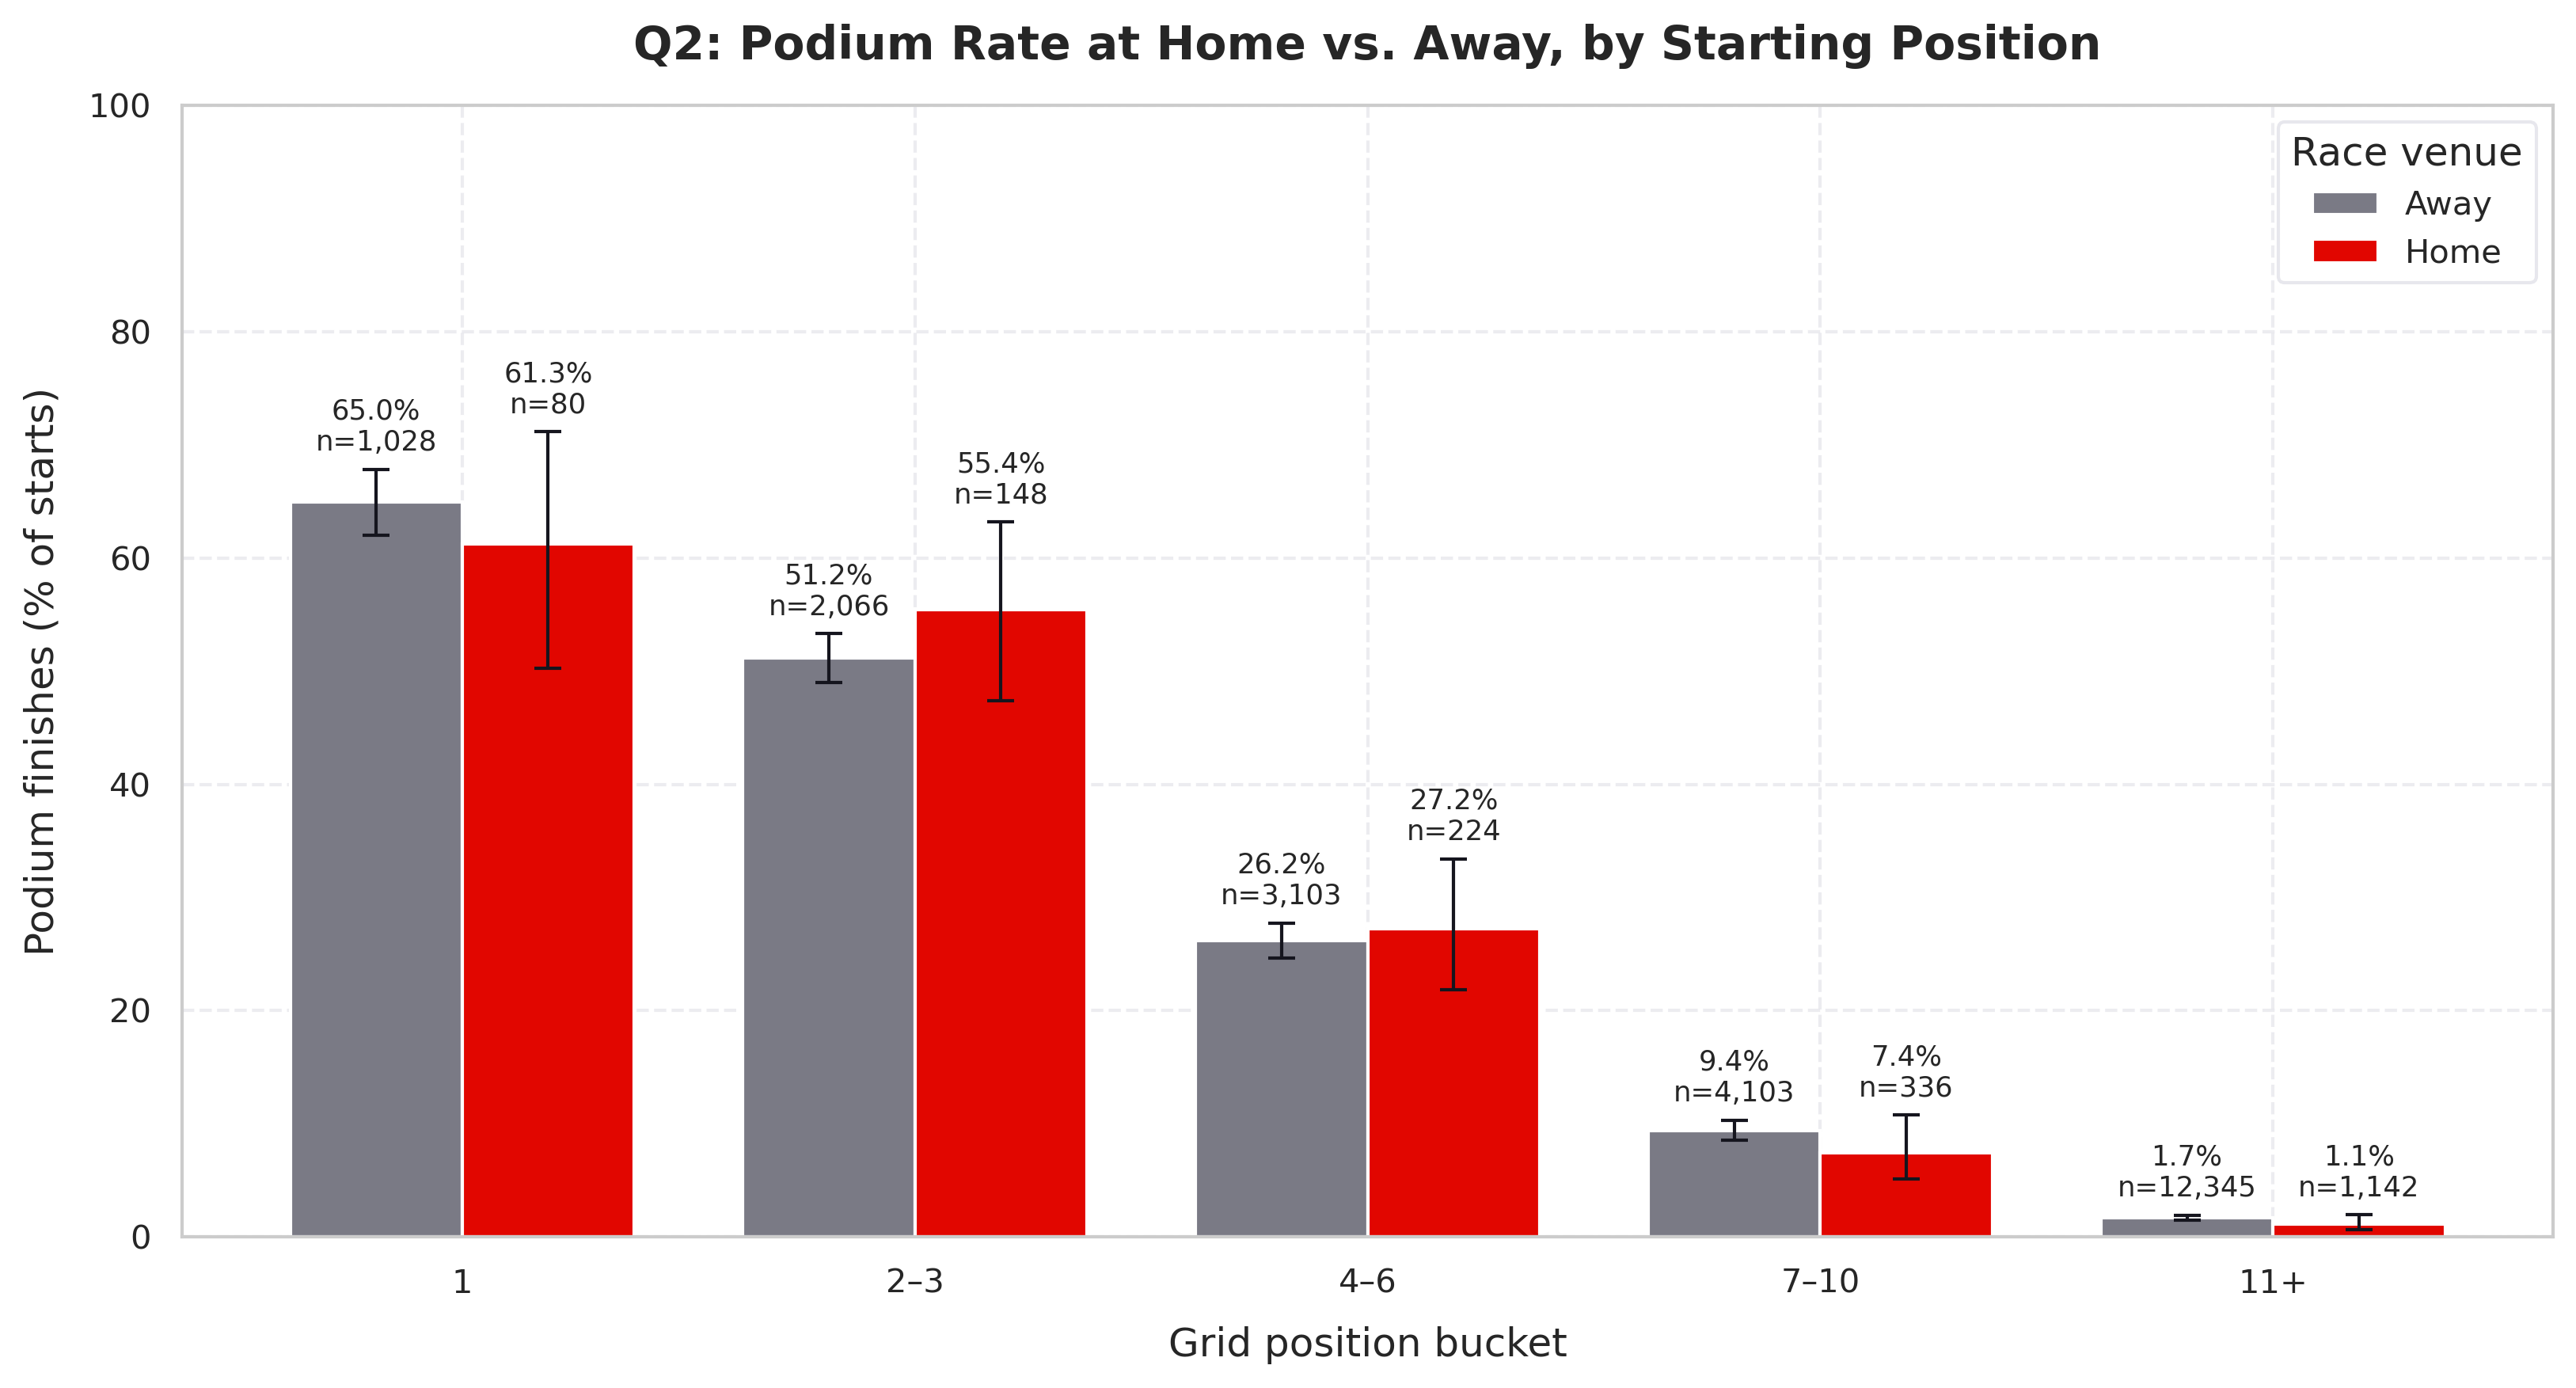
\includegraphics[width=\linewidth,height=0.42\textheight,keepaspectratio]{de_q2_home_advantage}
\caption{Podium rate at home and away within each grid bucket, with 95\% intervals.}
\end{figure}

{\small
\begin{xltabular}{\linewidth}{>{\raggedright\arraybackslash}X>{\raggedright\arraybackslash}X}
\toprule
\textbf{Joins} & \texttt{results} + \texttt{races} + \texttt{circuits} + \texttt{drivers} on \texttt{driverId} \\
\textbf{Grain} & One row per driver per race: 24,482 starts, of which 1,902 (7.8\%) are home starts \\
\textbf{Missing values} & Every nationality is mapped to its home countries (asserted, DEC-012) and no row lacks a grid slot. Drivers from countries without a circuit stay in the away group \\
\textbf{Pre-race cutoff} & Nationality, circuit country and grid slot are known before the start. \texttt{podium} is the outcome \\
\bottomrule
\end{xltabular}
}

\subsection{Q3: Which constructors have the highest mechanical-retirement rate in 2014–2021 and in 2022–2024?}

\textbf{Answer. 2014–2021: Lotus F1, Toro Rosso and Renault. 2022–2024: Alfa Romeo, Alpine and AlphaTauri.}

{\small
\begin{xltabular}{\linewidth}{>{\raggedright\arraybackslash}X>{\raggedright\arraybackslash}X>{\raggedright\arraybackslash}X}
\toprule
\textbf{Era} & \textbf{Highest rates (retirements of starts)} & \textbf{Lowest} \\
\midrule
\endhead
2014–2021 & Lotus F1 20.0\% (15 of 75), Toro Rosso 16.5\% (40 of 242), Renault 14.1\% (28 of 199) & Aston Martin 2.3\% (1 of 44), Alfa Romeo 4.2\% (5 of 120), Mercedes 4.4\% (14 of 320) \\
2022–2024 & Alfa Romeo 12.5\% (11 of 88), Alpine 10.4\% (14 of 135), AlphaTauri 8.0\% (7 of 88) & Sauber 2.1\% (1 of 48), Red Bull and McLaren 3.7\% (5 of 136) \\
\bottomrule
\end{xltabular}
}

\begin{itemize}
\item \textbf{Definition (DEC-036).} All 139 status values are mapped to one of four categories: finished, mechanical, accident or driver error, and regulatory or other. Following the instructors' ruling, \texttt{Puncture}, \texttt{Tyre}, \texttt{Tyre puncture}, \texttt{Fire} and \texttt{Safety belt} are mechanical and \texttt{Refuelling} is not; the mapping asserts this. A mechanical retirement is a start that ended with a failed car component. The denominator is race starts, not entries.
\item \textbf{Reliability improved across the field:} from 9.77\% of starts in 2014–2021 to 5.92\% in 2022–2024. Tyre failures add 11 retirements in 2014–2021 and none later; the top three of each era are the same with or without them.
\item \textbf{Same team across eras (DEC-014).} With renamed teams merged, the Lotus F1 / Renault / Alpine team is the least reliable in both eras. McLaren improved most, from 13.6\% to 3.7\%.
\item \textbf{Sensitivity.} Counting the generic \texttt{Retired} label as mechanical leaves the 2014–2021 ranking almost unchanged; in 2022–2024 Alfa Romeo stays first but the order below it moves.
\item \textbf{How far to trust it.} The intervals are wide, especially in 2022–2024, where the top three are separated by 4 to 7 retirements. The leaders are clear; the middle of each ranking is not.
\end{itemize}

\begin{figure}[htbp]
\centering
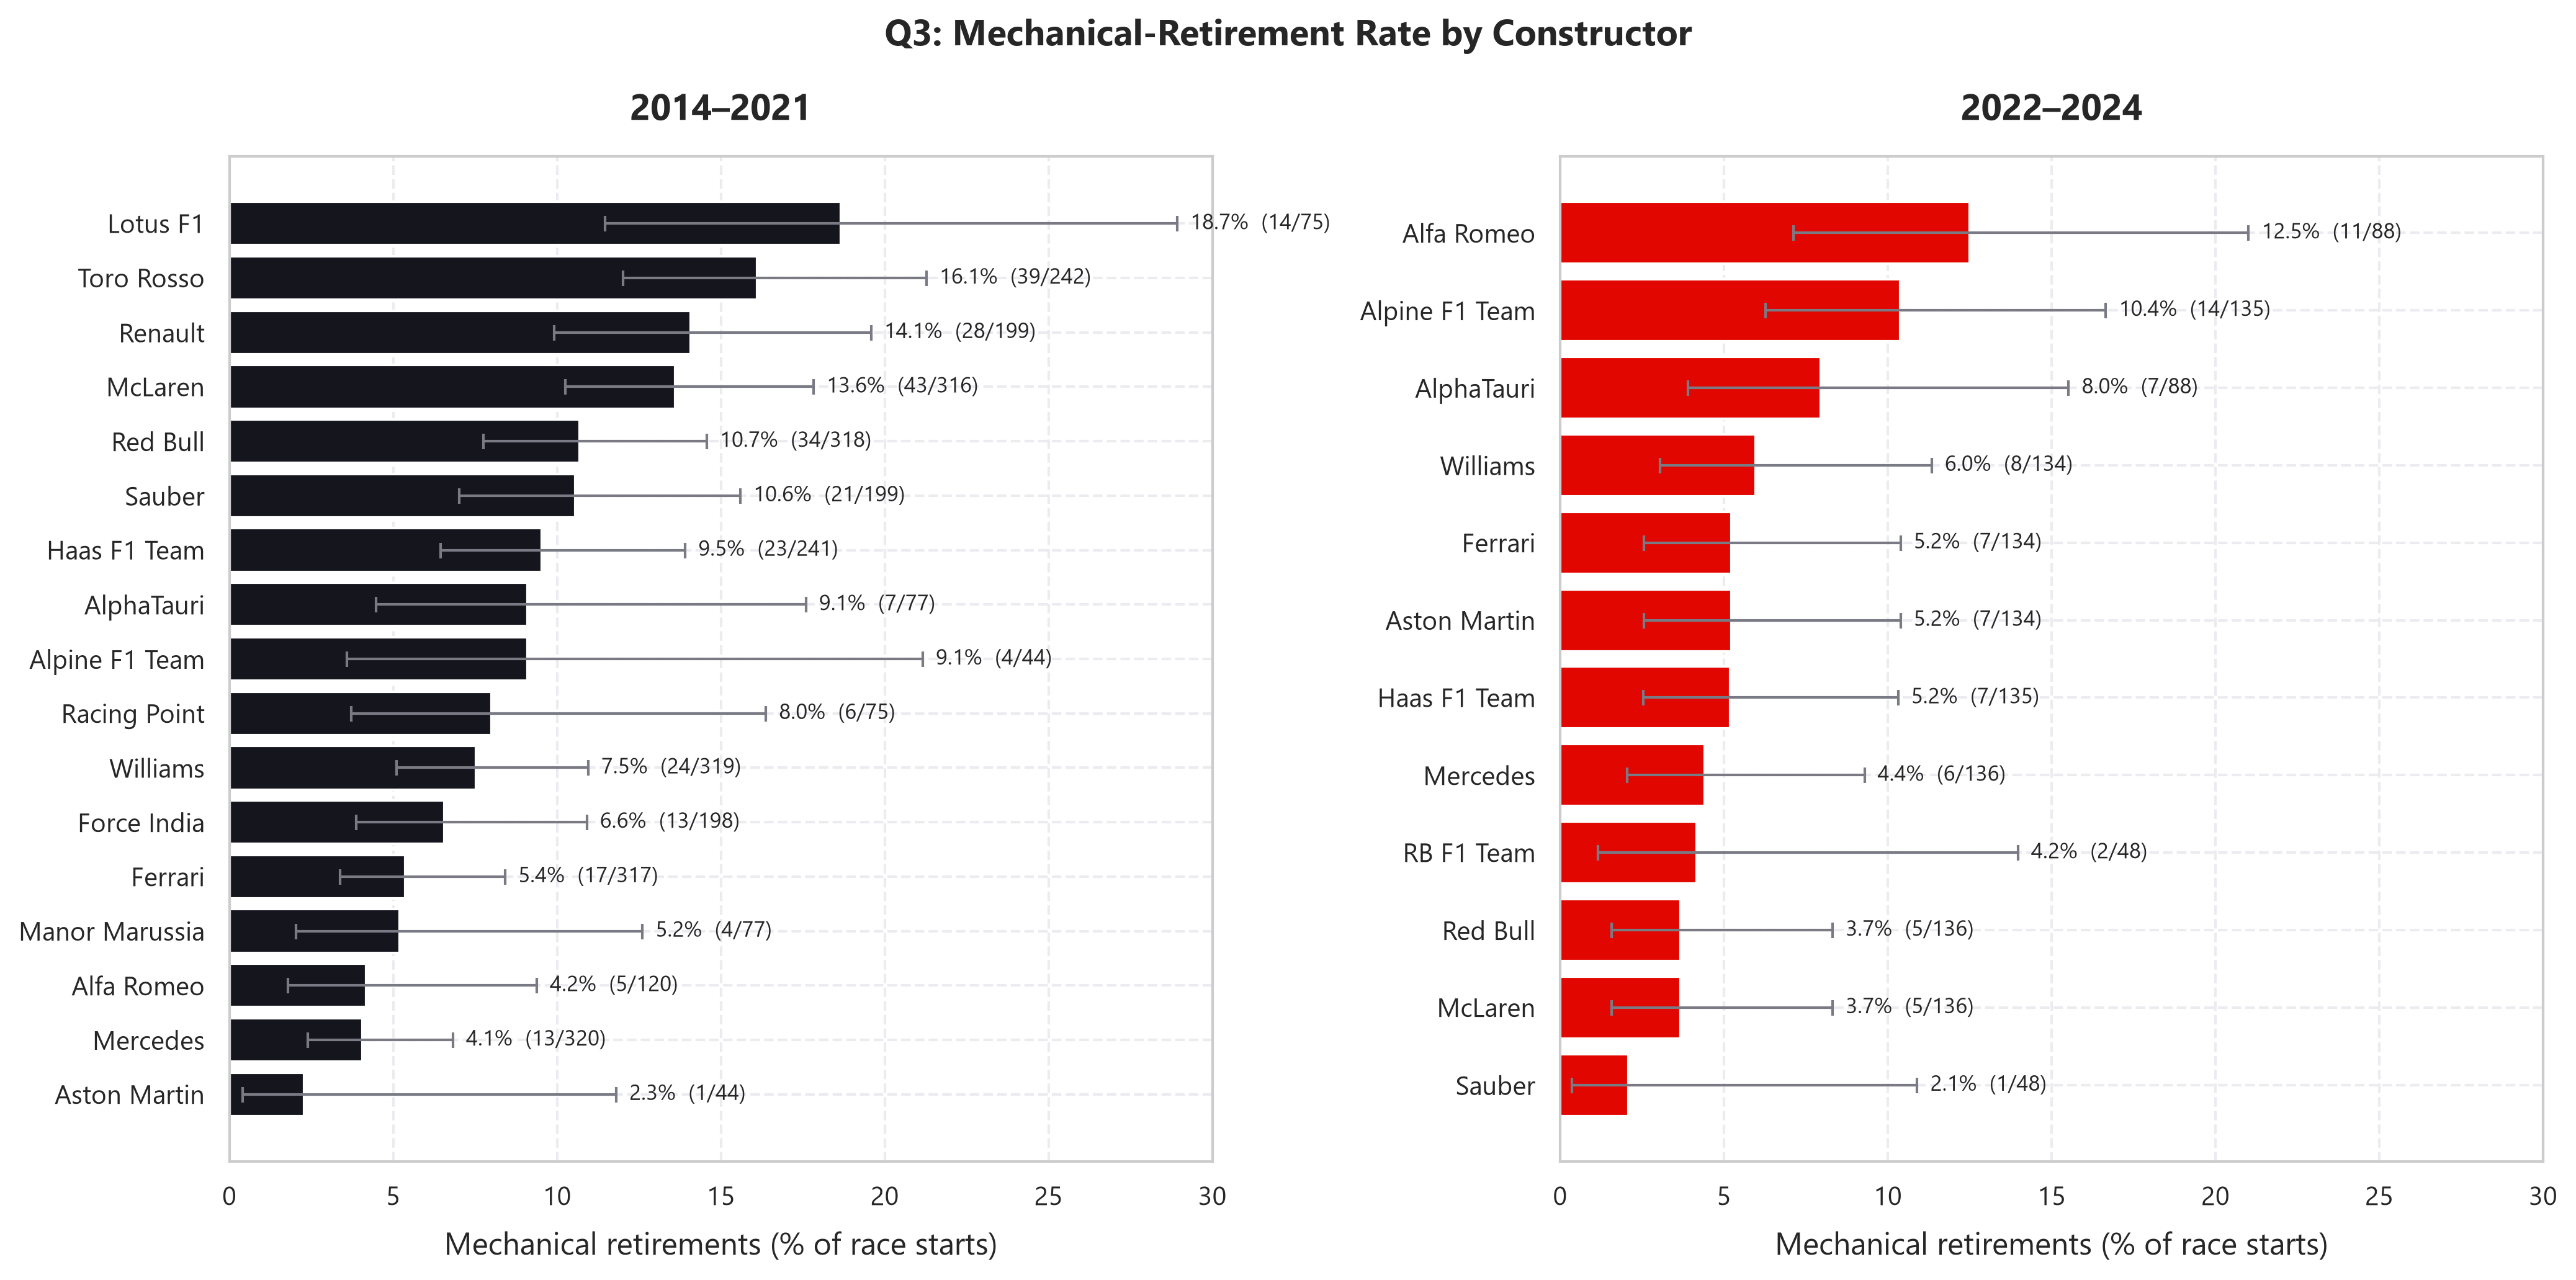
\includegraphics[width=\linewidth,height=0.42\textheight,keepaspectratio]{de_q3_mechanical_retirements}
\caption{Mechanical retirements per race start, per constructor and era, with 95\% intervals. Constructors with fewer than 40 starts in an era are not ranked.}
\end{figure}

{\small
\begin{xltabular}{\linewidth}{>{\raggedright\arraybackslash}X>{\raggedright\arraybackslash}X}
\toprule
\textbf{Joins} & \texttt{results} + \texttt{races} + \texttt{status} on \texttt{statusId} + \texttt{constructors} on \texttt{constructorId} \\
\textbf{Grain} & One row per driver per race start, aggregated per constructor and era; 4,597 starts from 2014 on \\
\textbf{Missing values} & Every status is mapped (asserted) and every row has a status and a constructor \\
\textbf{Pre-race cutoff} & \texttt{status} is recorded after the race and is used only as the outcome. As a model feature it would be allowed only as an aggregate of earlier races \\
\bottomrule
\end{xltabular}
}

\section{Features}

\subsection{Feature registry with temporal validity}

The modeling table has 21 features in six groups. The last column states why each value is known before the race starts.

{\small
\begin{xltabular}{\linewidth}{>{\raggedright\arraybackslash}X>{\raggedright\arraybackslash}X>{\raggedright\arraybackslash}X>{\raggedright\arraybackslash}X>{\raggedright\arraybackslash}X}
\toprule
\textbf{Group} & \textbf{Feature} & \textbf{Source tables} & \textbf{Definition} & \textbf{Why it is known before the race} \\
\midrule
\endhead
Grid & \texttt{grid} & results & Starting slot; pit-lane starts recoded behind the last car & Set after qualifying and penalties \\
 & \texttt{pit\_\allowbreak{}start} & results & 1 if the car started from the pit lane & Set before the start \\
 & \texttt{front\_\allowbreak{}row} & results & 1 if grid is 1 or 2 & Derived from grid \\
 & \texttt{teammate\_\allowbreak{}grid\_\allowbreak{}diff} & results & Grid slot minus the mean slot of the team's other cars & Derived from grid \\
Qualifying & \texttt{quali\_\allowbreak{}position} & qualifying & Qualifying classification, before grid penalties & Qualifying ends before the race \\
 & \texttt{gap\_\allowbreak{}to\_\allowbreak{}pole} & qualifying & Best of Q1–Q3, \% slower than the fastest qualifier & Qualifying ends before the race \\
 & \texttt{q3\_\allowbreak{}reached} & qualifying & 1 if a Q3 time was set & Qualifying ends before the race \\
 & \texttt{missing\_\allowbreak{}quali\_\allowbreak{}flag} & qualifying & 1 if the row has no qualifying record & Known from the data itself \\
Driver form & \texttt{driver\_\allowbreak{}rolling\_\allowbreak{}podium\_\allowbreak{}rate\_\allowbreak{}5} & results, races & Podium rate over the driver's last 5 races & Shifted by one race: earlier races only \\
 & \texttt{driver\_\allowbreak{}rolling\_\allowbreak{}avg\_\allowbreak{}finish\_\allowbreak{}5} & results, races & Mean finishing order over the last 5 races & Shifted by one race: earlier races only \\
 & \texttt{driver\_\allowbreak{}career\_\allowbreak{}podium\_\allowbreak{}rate} & results, races & Podium rate over all earlier races & Shifted by one race: earlier races only \\
Constructor form & \texttt{constructor\_\allowbreak{}rolling\_\allowbreak{}podium\_\allowbreak{}rate\_\allowbreak{}5} & results, races & Podiums per car entered over the team's last 5 races & Shifted by one race: earlier races only \\
 & \texttt{constructor\_\allowbreak{}rolling\_\allowbreak{}points\_\allowbreak{}5} & results, races & Team's share of all points awarded in its last 5 races & Shifted by one race: earlier races only \\
Standings & \texttt{driver\_\allowbreak{}pre\_\allowbreak{}race\_\allowbreak{}points} & driver\_standings, races & Driver's points as a share of the leader's, after the previous round & Standings of the previous round, same season \\
 & \texttt{driver\_\allowbreak{}pre\_\allowbreak{}race\_\allowbreak{}rank} & driver\_standings, races & Championship position after the previous round & Standings of the previous round, same season \\
 & \texttt{constructor\_\allowbreak{}pre\_\allowbreak{}race\_\allowbreak{}points} & constructor\_standings, races & Team's points as a share of the leader's, after the previous round & Standings of the previous round, same season \\
 & \texttt{constructor\_\allowbreak{}pre\_\allowbreak{}race\_\allowbreak{}rank} & constructor\_standings, races & Constructors' championship position after the previous round & Standings of the previous round, same season \\
Context & \texttt{field\_\allowbreak{}size} & results & Number of starters in the race & The grid is final before the start \\
 & \texttt{round} & races & Round number within the season & Calendar \\
 & \texttt{is\_\allowbreak{}home\_\allowbreak{}race} & drivers, circuits & 1 if the circuit is in the driver's home country & Static attributes \\
 & \texttt{circuit\_\allowbreak{}historical\_\allowbreak{}podium\_\allowbreak{}rate} & results, races & Driver's podium rate in earlier races at this circuit & Shifted by one race: earlier races only \\
\bottomrule
\end{xltabular}
}

Three design choices need a word:

\begin{itemize}
\item \textbf{Standings are taken from the previous round.} The dataset stores standings as they stood \emph{after} each race. Using the row of the same race would leak the result, so the row of round \emph{r − 1} is used for round \emph{r}.
\item \textbf{Points are shares, not totals (DEC-015).} A win was worth 8 to 10 points until 2009 and 25 from 2010. Dividing by the points awarded, or by the leader's points, keeps the feature on one scale across eras.
\item \textbf{Sprint results are left out (DEC-016), but not because they leak (DEC-039).} The instructors asked for a judgement on this. Every sprint is held the day before its Grand Prix, so its result is known before the race starts. In 2021–2022 the sprint set the grid (grid slot and sprint position agree for 55\% of starters, Spearman 0.94), so its information is already in \texttt{grid}. The leakage routes are guarded in code: every sprint column is prefixed (the sprint shares the Grand Prix \texttt{raceId}), standings come from the previous round (the standings after a sprint weekend include its sprint points), and no sprint column reaches the features. The group is left out because the training seasons contain no sprint at all.
\end{itemize}

\subsection{Proof that the features do not leak}

A written rule is not a proof, so the notebook tests the feature table directly.

\begin{itemize}
\item \textbf{A blacklist enforced in code.} Race-outcome columns (finishing position, points, laps, race time, fastest lap, status) are listed once, and \texttt{assert\_\allowbreak{}leakage\_\allowbreak{}safe()} rejects any feature list that contains one of them.
\item \textbf{Test 1, independent recomputation.} For 300 random rows, six history features are recomputed the slow way, using only rows with an earlier date. They match the feature table.
\item \textbf{Test 2, corrupting the future.} For 20 random races, every outcome from that race onward is scrambled and the feature table is rebuilt. The 21 features of that race do not change. A control feature built without the one-race shift is flagged in 20 of 20 races, which shows the test can detect leakage.
\item \textbf{Test 3, rebuilding at inference time.} The inference function builds features from the races before the requested one, with the requested race's results blanked. For 36 validation and test rows the rebuilt features and model scores are identical to the feature table (Section 9).
\end{itemize}

\subsection{Evidence behind the feature set}

\begin{itemize}
\item \textbf{Grid position is the strongest signal available for every row.} The podium rate falls from 63.3\% on pole to 5.8\% from tenth and 0.8\% from twentieth. Used alone, \texttt{grid} has a ROC-AUC of 0.884.
\item \textbf{Qualifying adds a little where it exists.} \texttt{quali\_\allowbreak{}position} (0.905) and \texttt{gap\_\allowbreak{}to\_\allowbreak{}pole} (0.887) rank podiums slightly better than \texttt{grid}, but they are present in only 37\% of the training rows.
\item \textbf{Form and standings carry real signal:} each of those features scores between 0.79 and 0.84 alone.
\item \textbf{Four features have almost none alone} (\texttt{pit\_\allowbreak{}start}, \texttt{is\_\allowbreak{}home\_\allowbreak{}race}, \texttt{round}, \texttt{missing\_\allowbreak{}quali\_\allowbreak{}flag}, ROC-AUC 0.50 to 0.51). \texttt{is\_\allowbreak{}home\_\allowbreak{}race} agrees with Q2. They were kept so the ablation could measure them properly; Section 7 confirms they add nothing.
\item \textbf{Several features overlap.} \texttt{quali\_\allowbreak{}position} and \texttt{grid} correlate at 0.98. This matters for how the ablation and the explanations must be read.
\item \textbf{A rolling window of 5 races is enough (DEC-018).} With the career rate alongside, the driver-form features reach 0.843 with 5 races and 0.846 with 10.
\end{itemize}

\begin{figure}[htbp]
\centering
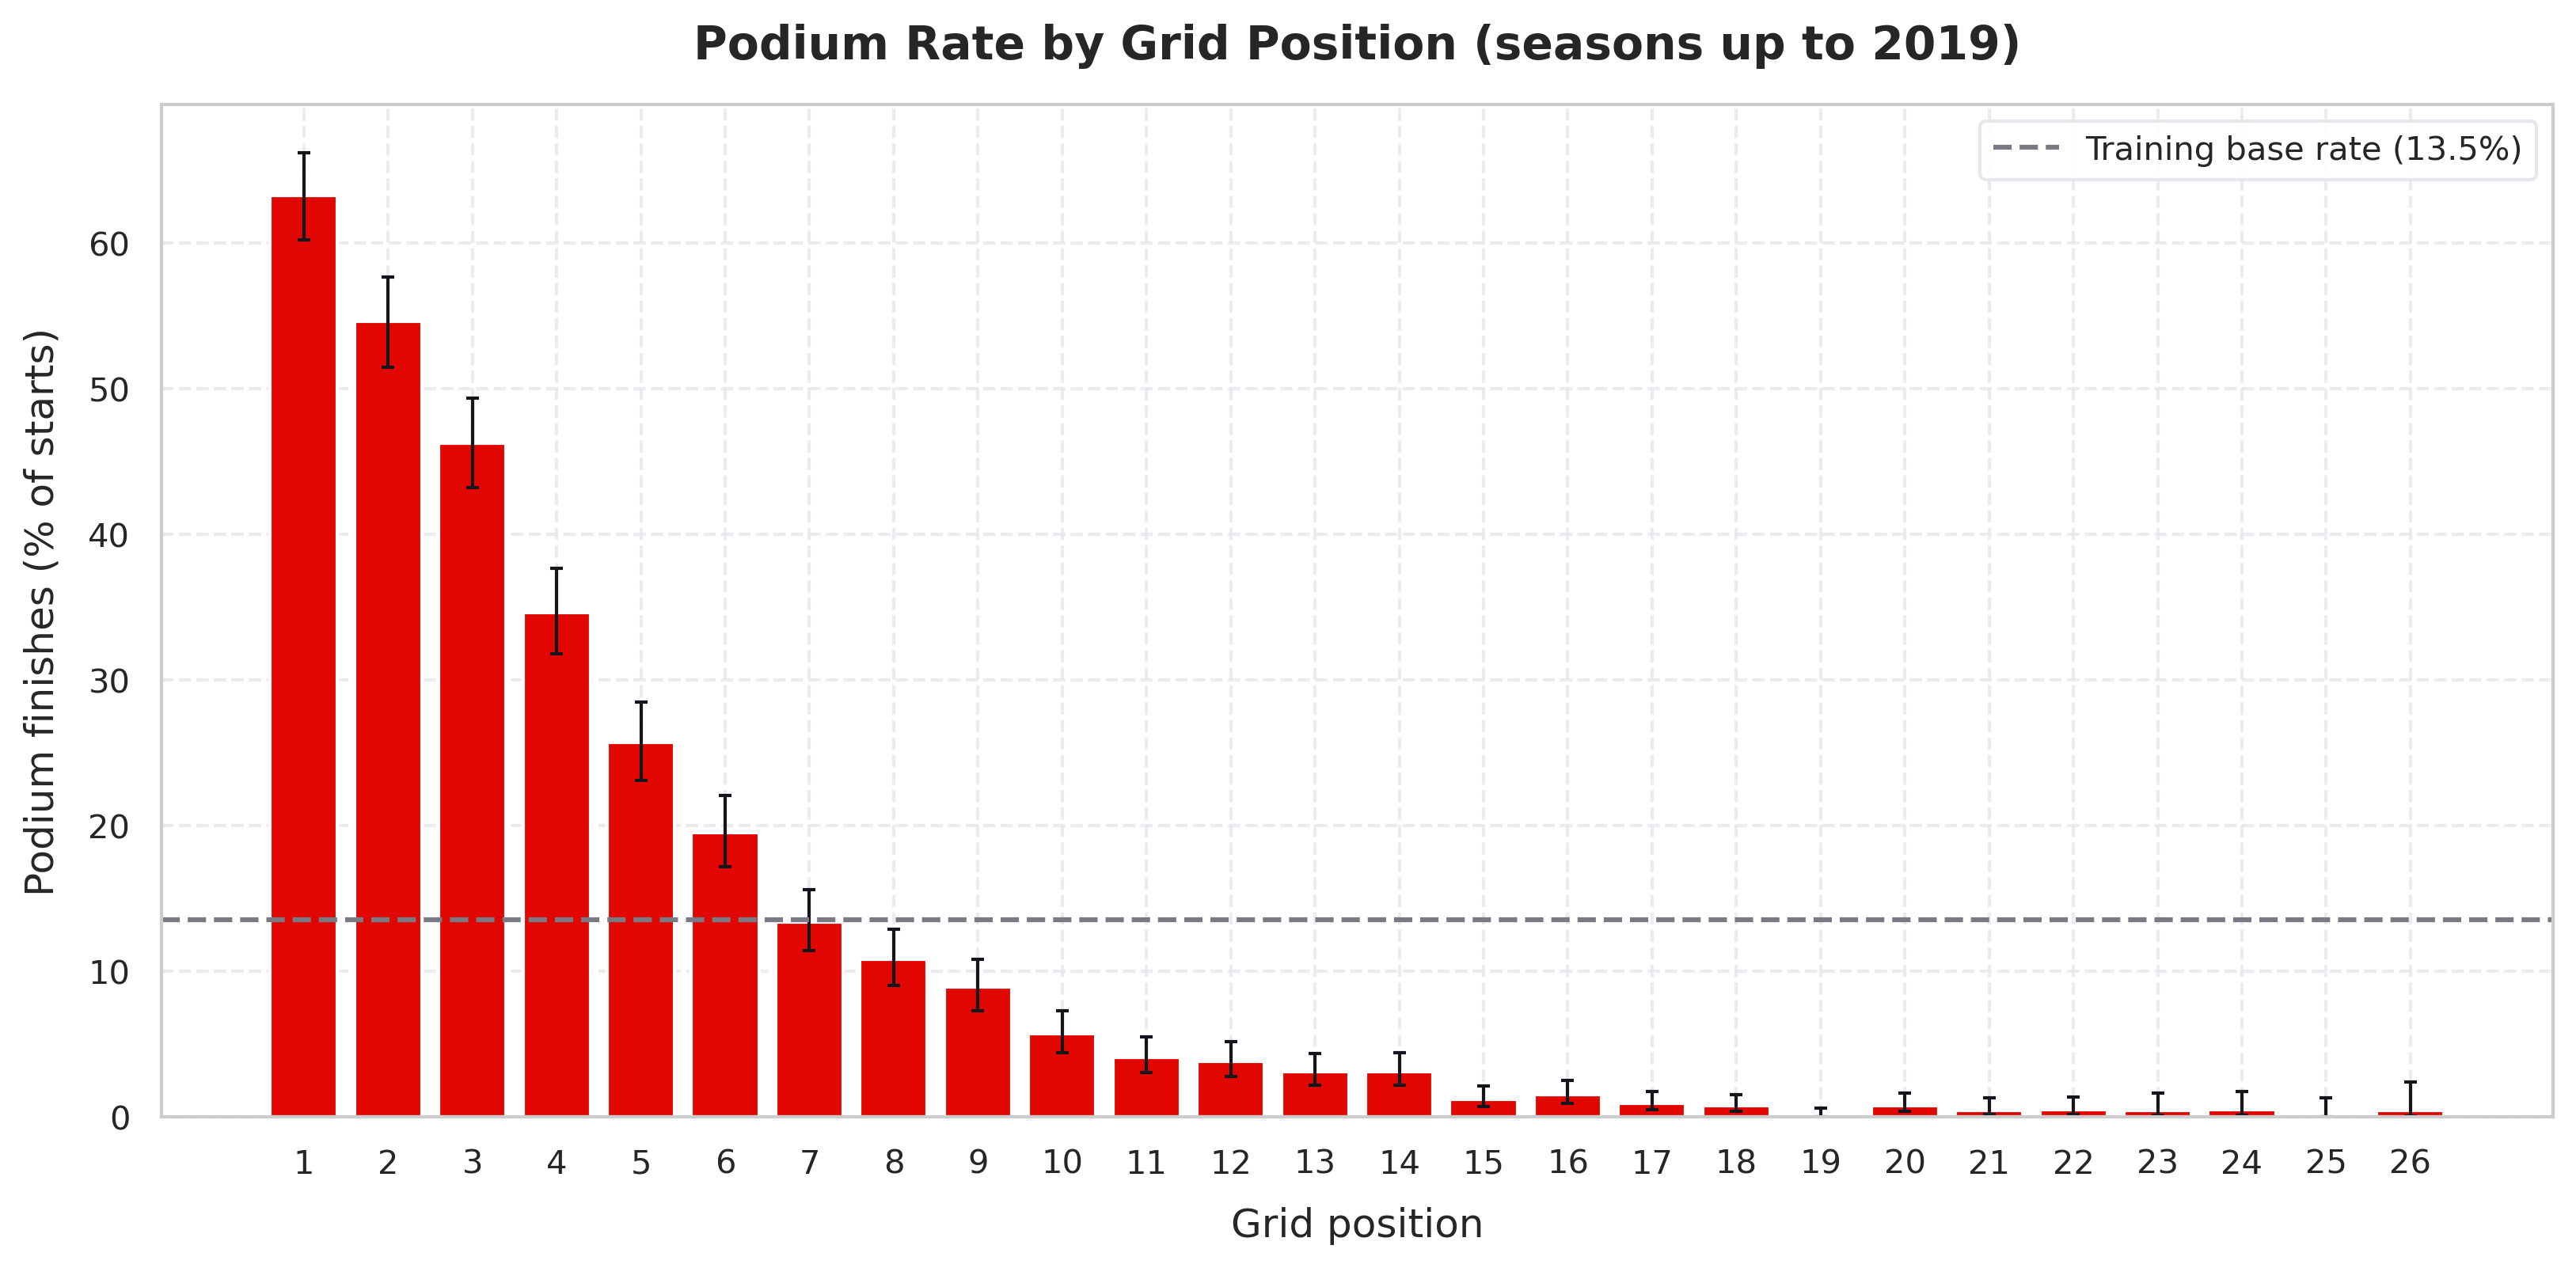
\includegraphics[width=\linewidth,height=0.42\textheight,keepaspectratio]{feat_podium_rate_by_grid}
\caption{Podium rate for each grid position in the training seasons, with 95\% intervals. The dashed line is the training base rate.}
\end{figure}

\begin{figure}[htbp]
\centering
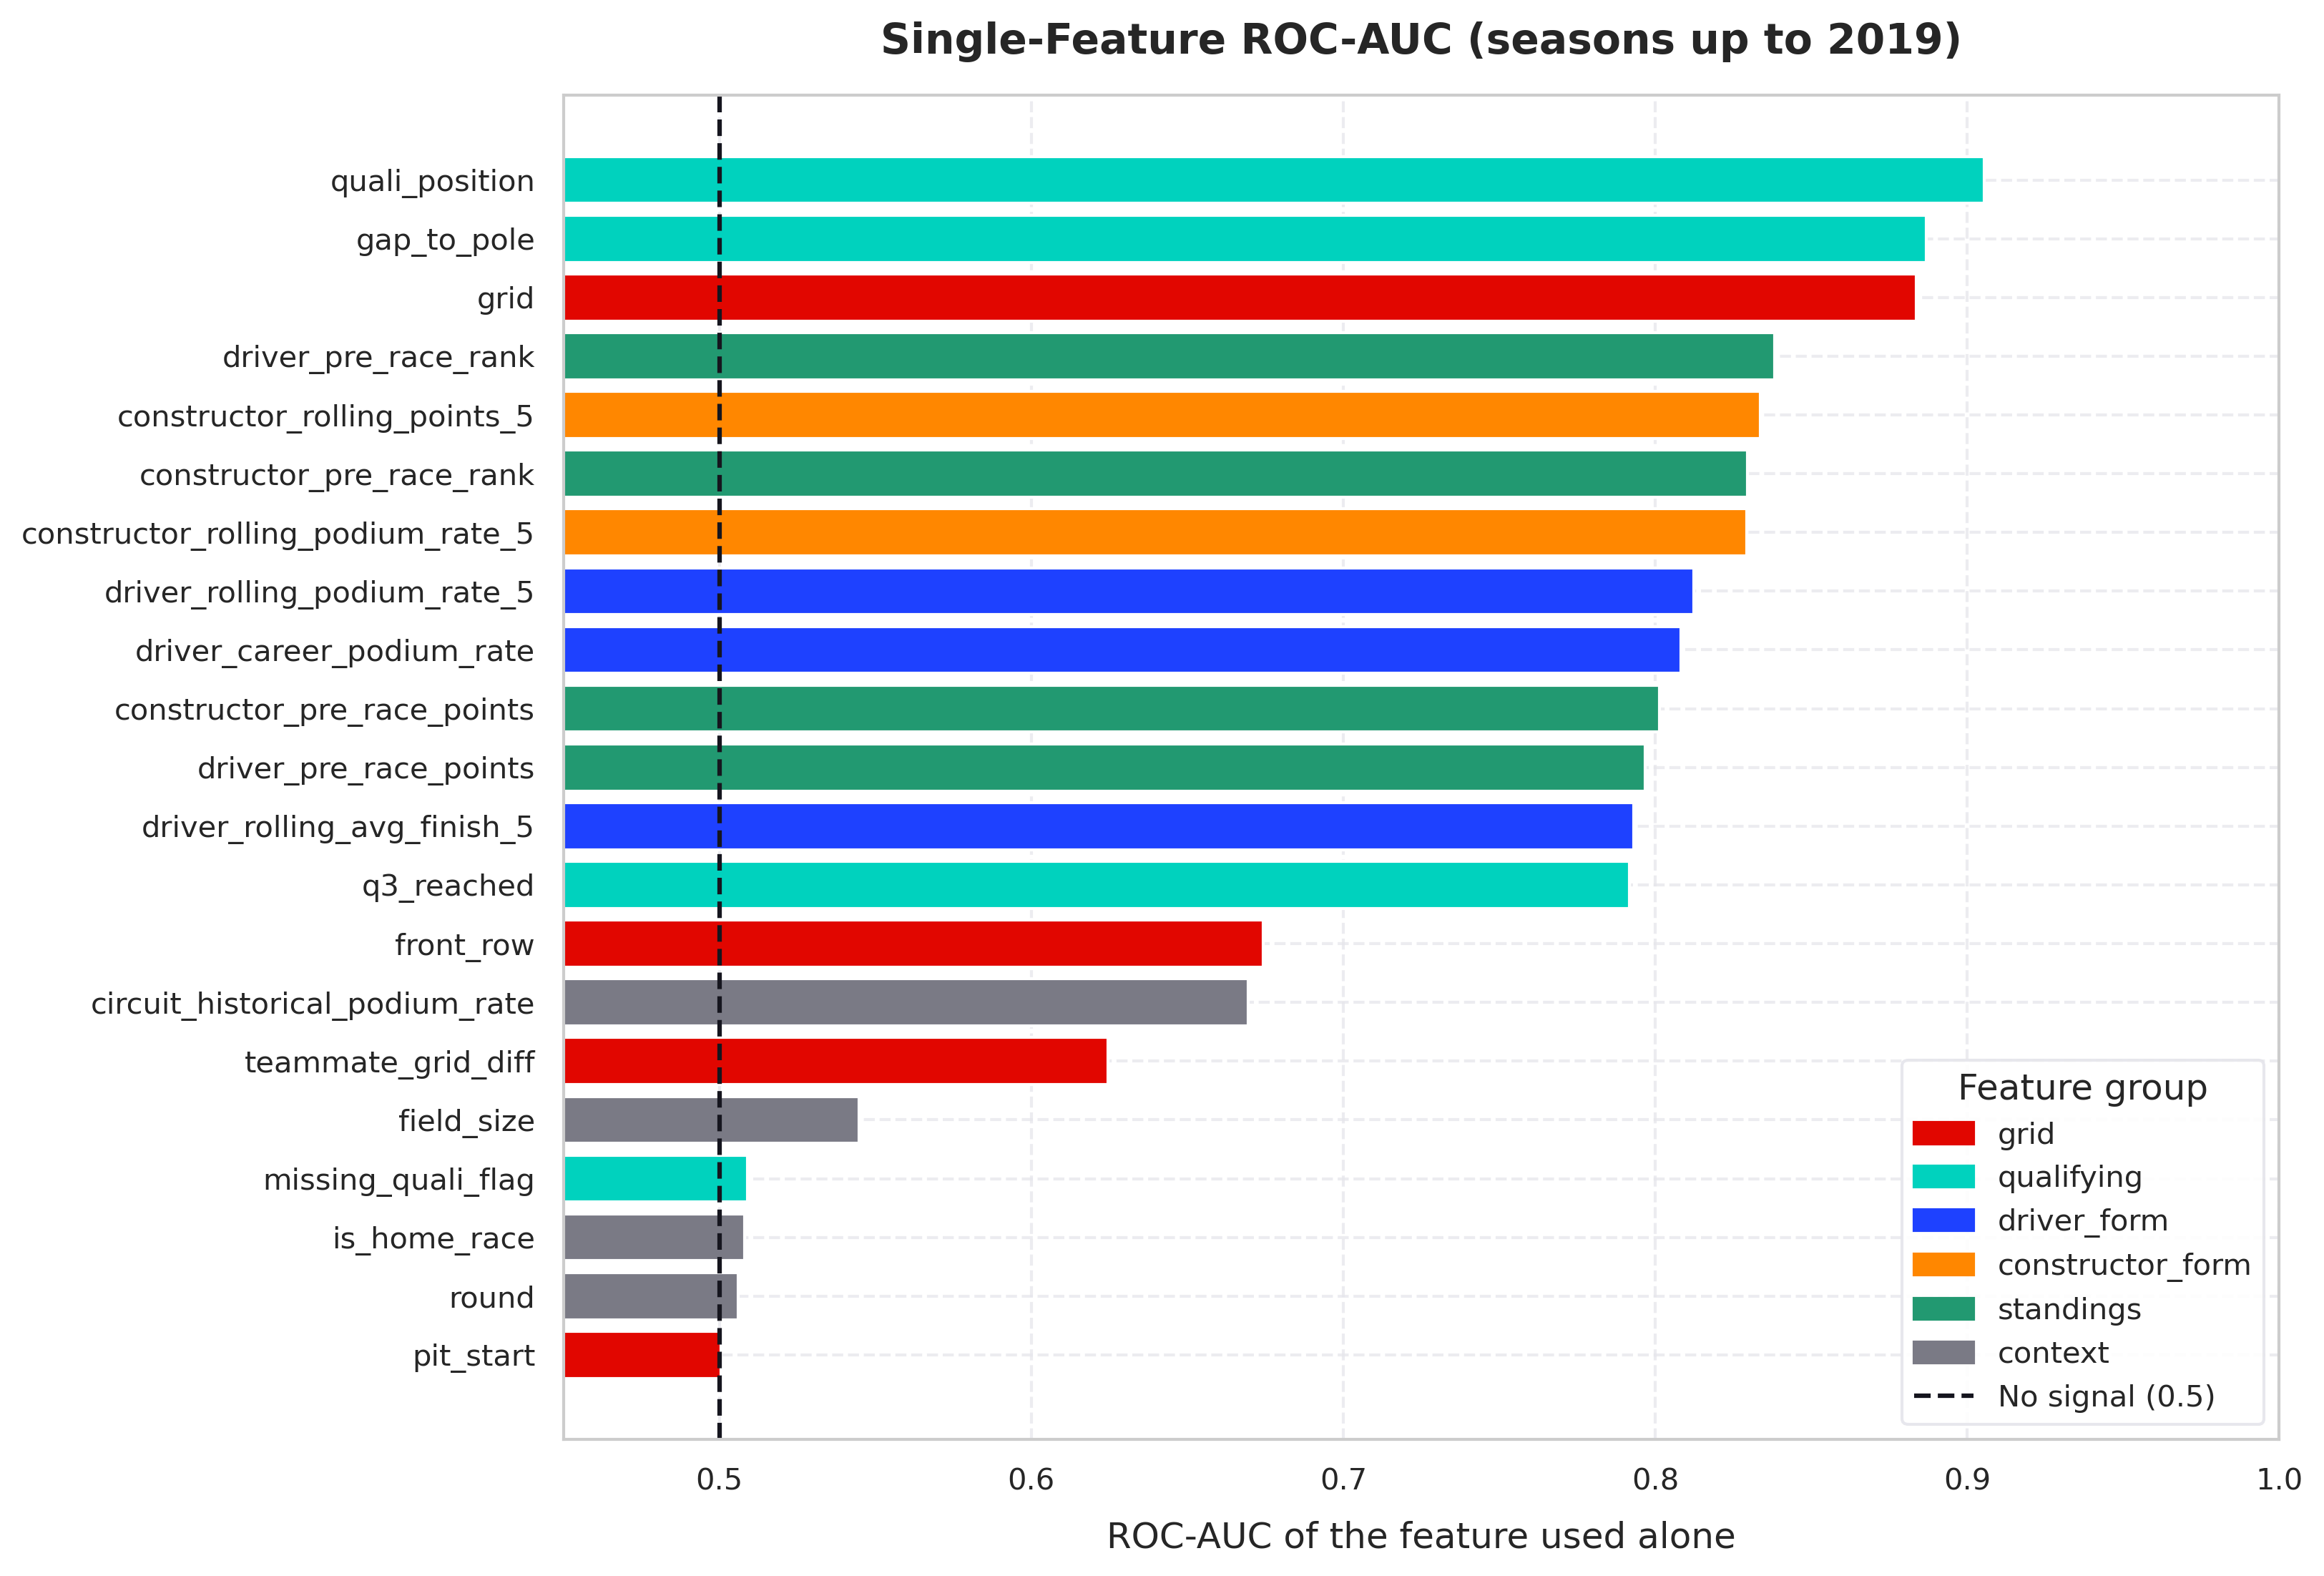
\includegraphics[width=\linewidth,height=0.42\textheight,keepaspectratio]{feat_univariate_auc}
\caption{ROC-AUC of each feature used alone, coloured by feature group. 0.5 is no signal.}
\end{figure}

\section{Split and Preprocessing}

\textbf{Pipeline.} For models that need complete, scaled inputs: a missing qualifying position is filled with the grid slot, the 16 continuous features are imputed with the training median and standardised, and a missing flag is filled with 0. Everything is fitted on the training seasons only. No encoder is needed (DEC-020): every feature is numeric or a 0/1 flag, and driver and team identifiers are not one-hot encoded, because many validation and test rows belong to drivers or teams that never appear in training.

\textbf{Training window (DEC-019).} Because qualifying is missing in 63\% of training rows, the window was tested instead of assumed.

{\small
\begin{xltabular}{\linewidth}{>{\raggedright\arraybackslash}Xrrr}
\toprule
\textbf{Training window} & \textbf{Train rows} & \textbf{Logistic regression, validation PR-AUC} & \textbf{Gradient boosting, validation PR-AUC} \\
\midrule
\endhead
All seasons & 22,355 & 0.726 & 0.713 \\
From 1994 & 10,091 & 0.720 & 0.704 \\
From 2003 & 6,782 & 0.725 & 0.693 \\
From 2006 & 5,743 & 0.728 & 0.665 \\
\bottomrule
\end{xltabular}
}

The window makes no real difference to the logistic regression and less data hurts gradient boosting, so all seasons are used. This also follows the instructors' rule that the whole dataset be used and old seasons not be dropped.

\textbf{Preprocessing-order experiments (DEC-021).} Both are scored on validation with a logistic regression, with a 95\% interval from resampling whole races 500 times.

{\small
\begin{xltabular}{\linewidth}{>{\raggedright\arraybackslash}X>{\raggedright\arraybackslash}X>{\raggedright\arraybackslash}X}
\toprule
\textbf{Experiment} & \textbf{Variants compared} & \textbf{Difference in validation PR-AUC (95\% interval)} \\
\midrule
\endhead
1. Scope of fitting & Preprocessor fitted on train only vs. on all rows & −0.0001 (−0.0004 to +0.0000) \\
2. Order of steps & Impute then scale vs. scale then impute & −0.0001 (−0.0007 to +0.0002) \\
\bottomrule
\end{xltabular}
}

Neither changes the score here, and the notebook shows why. In experiment 1 the validation and test seasons are only 8.7\% of the rows, so the fitted medians and standard deviations barely move. In experiment 2 the scaler does learn a different standard deviation (1.57 against 2.57 for \texttt{gap\_\allowbreak{}to\_\allowbreak{}pole}), but a logistic regression adjusts its coefficient to compensate. Fitting on train only and imputing first are kept because they are correct by construction, not because they score higher.

\textbf{Distribution shift.} Validation and test are not distributed like training: \texttt{field\_\allowbreak{}size} sits almost one training standard deviation below the training mean (modern grids have 20 cars) and \texttt{round} is higher (longer seasons). This is a reason to validate on recent seasons.

\begin{figure}[htbp]
\centering
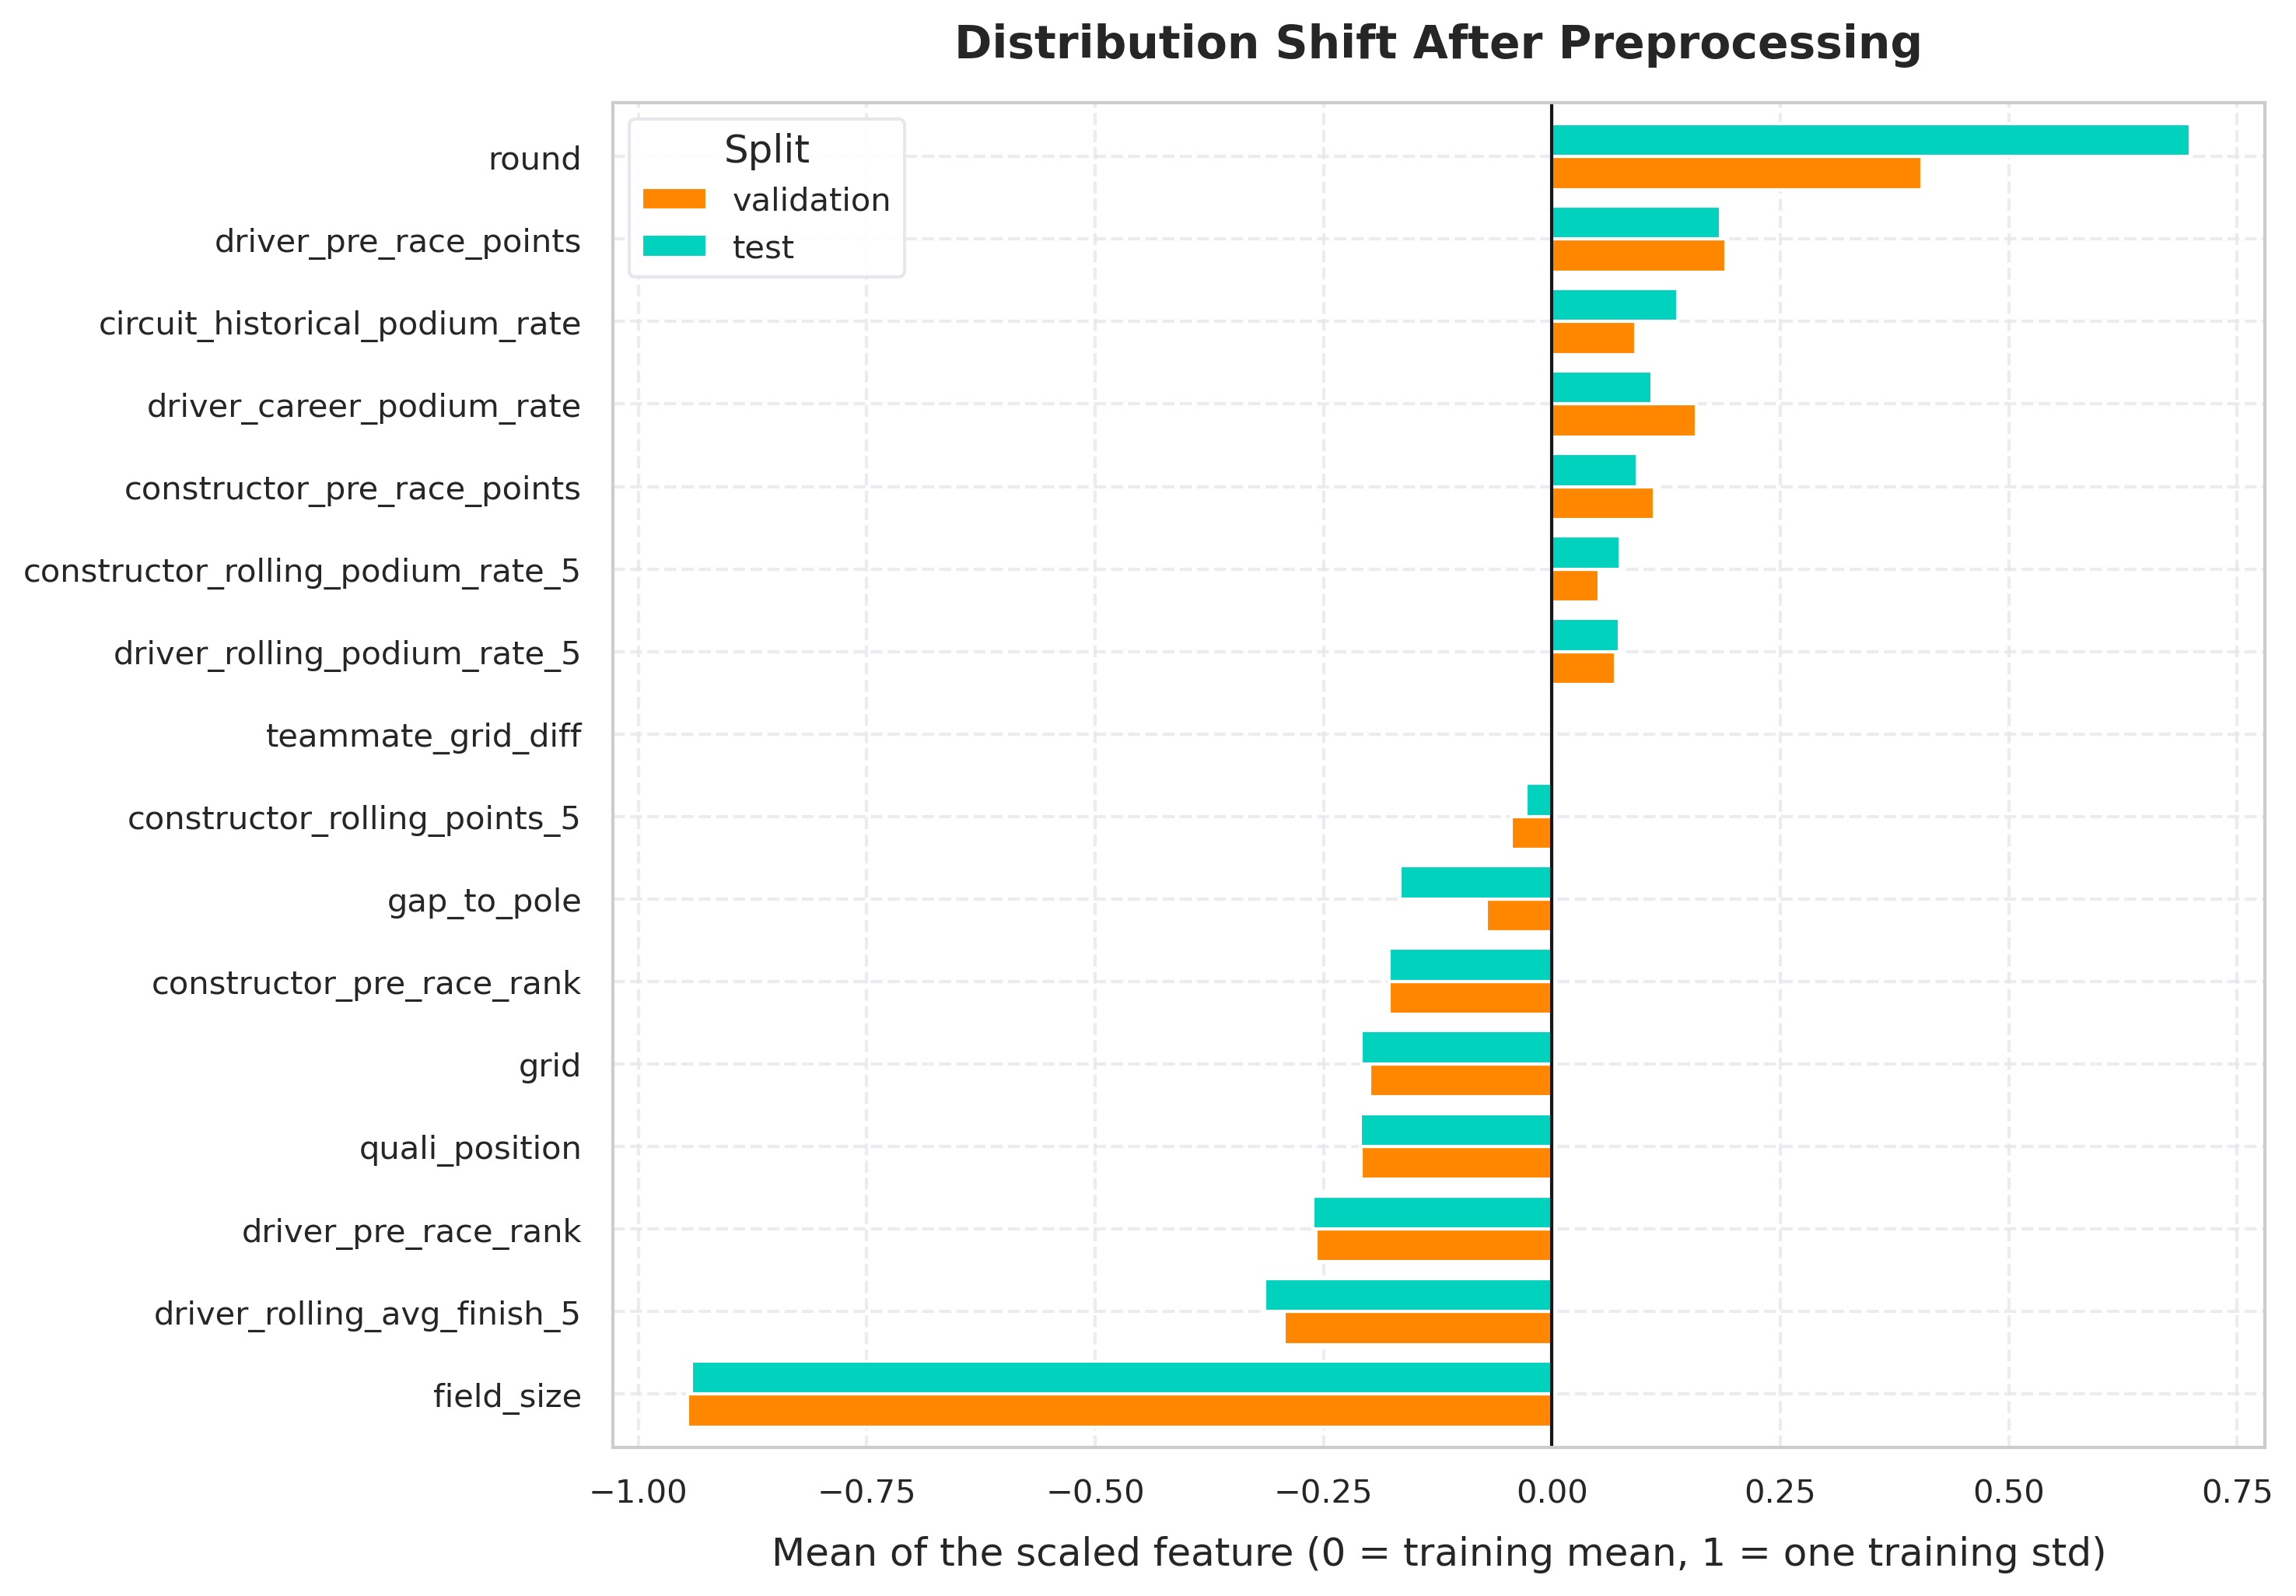
\includegraphics[width=\linewidth,height=0.42\textheight,keepaspectratio]{prep_distribution_shift}
\caption{Mean of each scaled feature in the validation and test seasons. Zero is the training mean.}
\end{figure}

\section{Models}

\subsection{Protocol}

\begin{itemize}
\item \textbf{Main metric: PR-AUC.} About 15\% of rows are podiums. PR-AUC measures how well a model ranks those few positives without needing a threshold. ROC-AUC is reported beside it but moves little, because it also rewards ranking the many easy back-of-grid rows.
\item \textbf{Secondary metric: F1} at a decision threshold, with precision and recall. The threshold of each model is the one with the highest F1 on validation (DEC-028).
\item \textbf{Every model is fitted on the training seasons only, and every choice is made on validation:} hyperparameters, the network's stopping epoch, the thresholds and the selected model. The test seasons were scored once for the comparison below, after all of those were fixed (DEC-030).
\item \textbf{Uncertainty.} Differences between models are given a 95\% interval by resampling whole races 500 times.
\item \textbf{Tuning is averaged over seeds (DEC-037).} Every hyperparameter configuration and network architecture is fitted with five random seeds and ranked by its mean validation PR-AUC. With one seed per configuration, removing 157 shared-drive rows was enough to change the winner of all three searches: the configurations at the top are closer together than the seed-to-seed noise, so a single-seed search rewards a lucky seed.
\end{itemize}

\subsection{The five models}

{\small
\begin{xltabular}{\linewidth}{>{\raggedright\arraybackslash}X>{\raggedright\arraybackslash}X>{\raggedright\arraybackslash}X}
\toprule
\textbf{Model} & \textbf{Input} & \textbf{Tuning} \\
\midrule
\endhead
Grid ≤ 3 rule (baseline) & \texttt{grid} only & None: predicts a podium for the first three grid slots \\
Logistic regression (baseline) & 21 preprocessed features & None. \texttt{C} from 0.01 to 100 gives 0.726 throughout \\
Random forest & 21 preprocessed features & 20 random configurations × 5 seeds; the best has trees of depth 4 \\
LightGBM (gradient boosting) & 21 raw features, missing values included & 40 random configurations × 5 seeds; the best has 100 trees of 8 leaves. Missing values are routed by the trees; imputing them instead scores no better (−0.004, interval −0.020 to +0.011) \\
Shallow neural network (Keras) & 21 preprocessed features & 8 architectures × 5 seeds; the best has two hidden layers (64 and 32 units), dropout 0.2, early stopping on validation PR-AUC \\
\bottomrule
\end{xltabular}
}

All learned models use balanced class weights. Measured directly (DEC-027), the weights do not change the ranking, but they double the model output: the result is a score, not a probability. Section 9 returns to this.

\subsection{Results on all three splits}

{\small
\begin{xltabular}{\linewidth}{>{\raggedright\arraybackslash}X>{\raggedright\arraybackslash}Xrrrrr}
\toprule
\textbf{Model} & \textbf{Split} & \textbf{ROC-AUC} & \textbf{PR-AUC} & \textbf{F1} & \textbf{Precision} & \textbf{Recall} \\
\midrule
\endhead
Grid ≤ 3 rule & Train & 0.884 & 0.500 & 0.545 & 0.545 & 0.545 \\
 & Validation & 0.910 & 0.648 & 0.695 & 0.698 & 0.692 \\
 & Test & 0.913 & 0.647 & 0.649 & 0.650 & 0.647 \\
Logistic regression & Train & 0.901 & 0.562 & 0.569 & 0.441 & 0.804 \\
 & Validation & 0.929 & 0.726 & 0.711 & 0.628 & 0.821 \\
 & Test & 0.937 & 0.712 & 0.670 & 0.528 & 0.917 \\
Random forest & Train & 0.906 & 0.587 & 0.587 & 0.529 & 0.660 \\
 & Validation & 0.930 & 0.735 & 0.710 & 0.680 & 0.744 \\
 & Test & 0.938 & 0.707 & 0.671 & 0.598 & 0.765 \\
LightGBM & Train & 0.909 & 0.590 & 0.587 & 0.535 & 0.649 \\
 & Validation & 0.931 & 0.743 & 0.711 & 0.697 & 0.727 \\
 & Test & 0.939 & 0.709 & 0.684 & 0.616 & 0.770 \\
Neural network & Train & 0.907 & 0.585 & 0.590 & 0.522 & 0.680 \\
 & Validation & 0.926 & 0.733 & 0.710 & 0.672 & 0.752 \\
 & Test & 0.937 & 0.720 & 0.675 & 0.590 & 0.789 \\
\bottomrule
\end{xltabular}
}

Test PR-AUC compared with the logistic regression: random forest −0.005 (95\% interval −0.034 to +0.022), LightGBM −0.003 (−0.030 to +0.021), neural network +0.009 (−0.009 to +0.025), grid rule −0.064 (−0.118 to −0.011).

\subsection{What the results say}

\begin{itemize}
\item \textbf{The features are worth about 0.06 PR-AUC over the grid rule.} This is the only difference in the table whose interval excludes zero.
\item \textbf{Model complexity adds nothing measurable.} The untuned logistic regression is level with the forest and LightGBM on test. The network scores highest, but by less than the width of its interval. This answers the brief's question of whether model complexity is justified: on this data it is not.
\item \textbf{Tuning on a small validation set flattered the forest and LightGBM.} From validation to test the logistic regression loses 0.015, the forest 0.028, LightGBM 0.034 and the network 0.013. The two models picked as the best of 20 and 40 configurations fall furthest.
\item \textbf{Training scores are the lowest in every row.} The training seasons run from 1950, have a lower podium rate and mostly lack qualifying data, so they are harder to predict than 2020–2024. No model has a training score far above its validation score, so none is overfitted.
\item \textbf{The tuned thresholds are too low for the test seasons.} They predict 3.8 to 5.2 podiums per race where there are 3. Picking the three highest-scoring drivers of each race instead gets about two of the three places right, the same as the grid rule.
\item \textbf{LightGBM is carried forward (DEC-029).} The rule was fixed before the test seasons were scored: the highest validation PR-AUC. On test it equals the logistic regression, which would be an equally defensible and simpler choice. The selection was not revisited after seeing the test scores.
\end{itemize}

\begin{figure}[htbp]
\centering
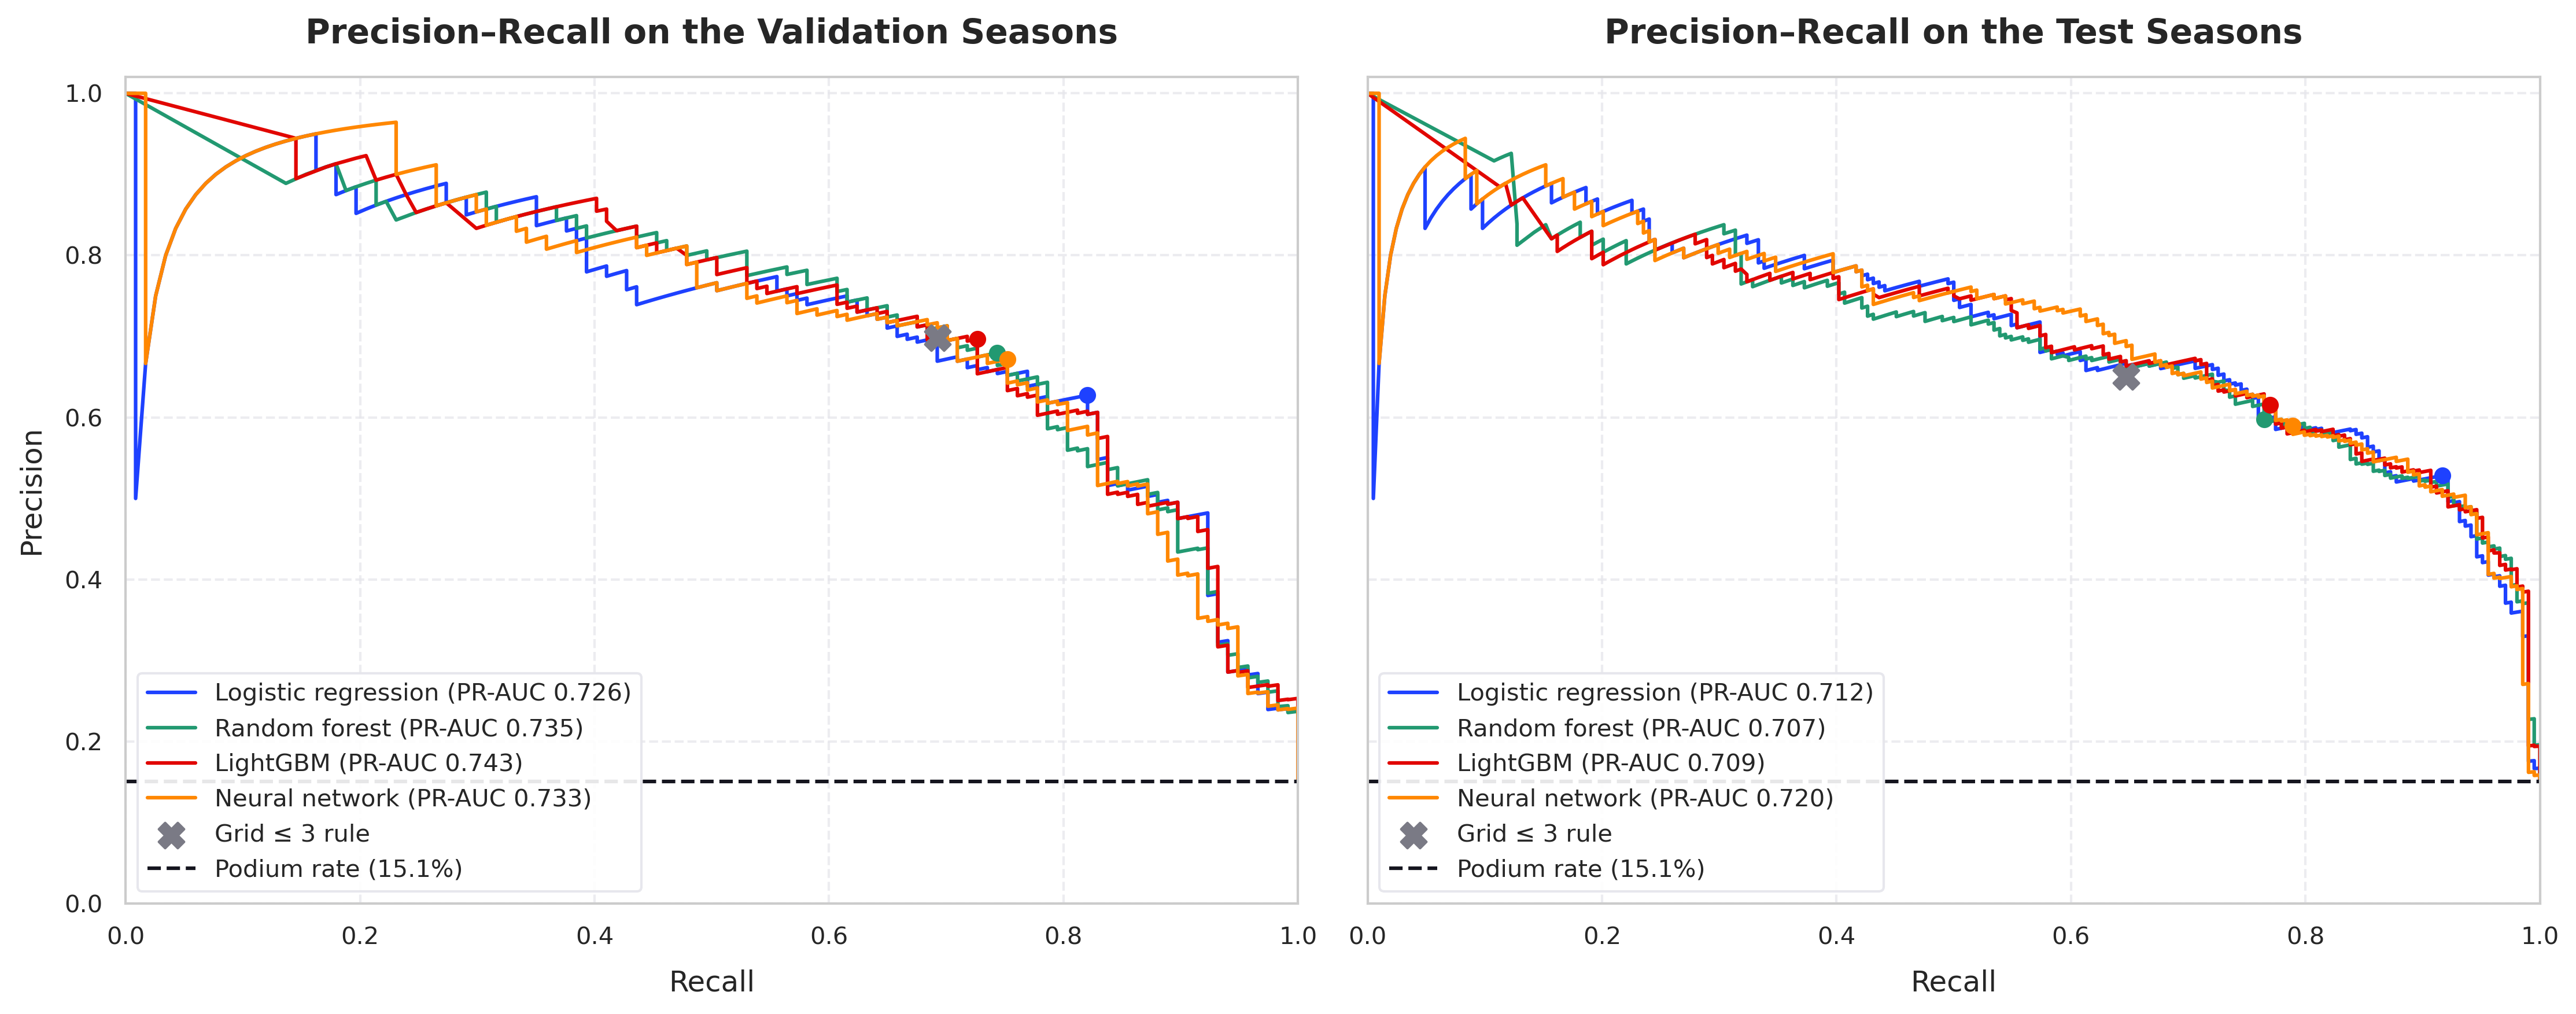
\includegraphics[width=\linewidth,height=0.42\textheight,keepaspectratio]{model_pr_curves}
\caption{Precision against recall on the validation and test seasons. The dot on each line is the model at its tuned threshold; the cross is the grid rule.}
\end{figure}

\section{Ablation}

LightGBM is retrained with part of the features removed. Only the columns change: the same hyperparameters, the same training rows, no retuning (DEC-031). Each difference comes with a 95\% interval from resampling races, and is also averaged over 10 random seeds, because the seed alone moves PR-AUC by about 0.005 on validation and 0.010 on test.

\textbf{Leave one group out.} No single group is significant: every interval includes zero on both splits.

{\small
\begin{xltabular}{\linewidth}{>{\raggedright\arraybackslash}X>{\raggedright\arraybackslash}X>{\raggedright\arraybackslash}X}
\toprule
\textbf{Removed group} & \textbf{Validation change in PR-AUC (95\% interval)} & \textbf{Test change in PR-AUC (95\% interval)} \\
\midrule
\endhead
Grid & −0.017 (−0.042 to +0.006) & −0.018 (−0.041 to +0.002) \\
Qualifying & −0.015 (−0.049 to +0.012) & +0.014 (−0.002 to +0.028) \\
Standings & −0.006 (−0.019 to +0.006) & +0.000 (−0.011 to +0.011) \\
Driver form & −0.005 (−0.016 to +0.007) & −0.005 (−0.023 to +0.017) \\
Constructor form & −0.003 (−0.013 to +0.005) & −0.002 (−0.010 to +0.005) \\
Context & −0.000 (−0.009 to +0.011) & +0.002 (−0.004 to +0.009) \\
\bottomrule
\end{xltabular}
}

This does not mean the features are useless. Leave-one-out measures what a group adds on top of all the others, and the groups overlap: grid and qualifying both say where the car starts; driver form, constructor form and standings all say how the driver and team have been doing. When one is removed, the model reads the same information from its neighbour. So the overlapping groups were also removed together, as blocks.

{\small
\begin{xltabular}{\linewidth}{>{\raggedright\arraybackslash}Xr>{\raggedright\arraybackslash}X>{\raggedright\arraybackslash}X}
\toprule
\textbf{Removed block} & \textbf{Features} & \textbf{Validation change (95\% interval)} & \textbf{Test change (95\% interval)} \\
\midrule
\endhead
Starting position (grid + qualifying) & 8 & −0.085 (−0.145 to −0.035) & −0.121 (−0.175 to −0.071) \\
Past results (driver form + constructor form + standings) & 9 & −0.064 (−0.108 to −0.018) & −0.031 (−0.065 to +0.006) \\
Context & 4 & −0.000 (−0.009 to +0.011) & +0.002 (−0.004 to +0.009) \\
\bottomrule
\end{xltabular}
}

\begin{itemize}
\item \textbf{Starting position is the larger block.} Removing it costs a clear amount on both splits. Alone it scores 0.670 on validation and 0.667 on test, about 0.02 above the grid rule.
\item \textbf{Past results add about 0.03 to 0.06 on top.} The evidence is firm on validation (the interval excludes zero) and weaker on test, where the selected model's interval reaches zero but the average over 10 seeds still loses 0.043. This is the gain Section 6 found between the grid rule and the learned models.
\item \textbf{Context adds nothing} and could be dropped. It was kept because the model was fixed before the test seasons were scored.
\item \textbf{History transfers less well than the starting position.} Alone, the starting position scores about the same on both splits, while past results fall from 0.652 on validation to 0.591 on test.
\end{itemize}

\textbf{Cleaning choices tested by retraining (DEC-038).} The two removals the instructors asked to be evidenced were reversed one at a time: the modeling table was rebuilt with the rows kept, and LightGBM and the logistic regression were retrained and compared on the same validation and test rows. A removal stands unless keeping the rows makes the model measurably better on validation.

{\small
\begin{xltabular}{\linewidth}{>{\raggedright\arraybackslash}X>{\raggedright\arraybackslash}X>{\raggedright\arraybackslash}X>{\raggedright\arraybackslash}X>{\raggedright\arraybackslash}X}
\toprule
\textbf{Rows kept} & \textbf{LightGBM, validation (95\% interval)} & \textbf{LightGBM, test (95\% interval)} & \textbf{LightGBM, 10-seed average (validation / test)} & \textbf{Logistic regression (validation / test)} \\
\midrule
\endhead
Withdrawn entries & −0.013 (−0.029 to −0.001) & +0.006 (−0.001 to +0.015) & −0.007 / −0.001 & +0.000 / −0.001 \\
Indianapolis 500 & −0.000 (−0.004 to +0.003) & +0.000 (−0.003 to +0.003) & −0.000 / +0.001 & −0.001 / +0.001 \\
\bottomrule
\end{xltabular}
}

\begin{itemize}
\item \textbf{The Indianapolis 500 makes no difference} to either model on either split. Its exclusion is a scope decision without measurable effect: 11 oval races run to other rules, whose drivers (103 of 107) never started another championship race. The 1950–1960 seasons stay in the data.
\item \textbf{The withdrawn entries make LightGBM worse on validation}, by more than the seed noise, and change nothing elsewhere. Keeping them adds races without a podium to the history of drivers who never took the start. The model is better without them, so the removal stands.
\end{itemize}

\begin{figure}[htbp]
\centering
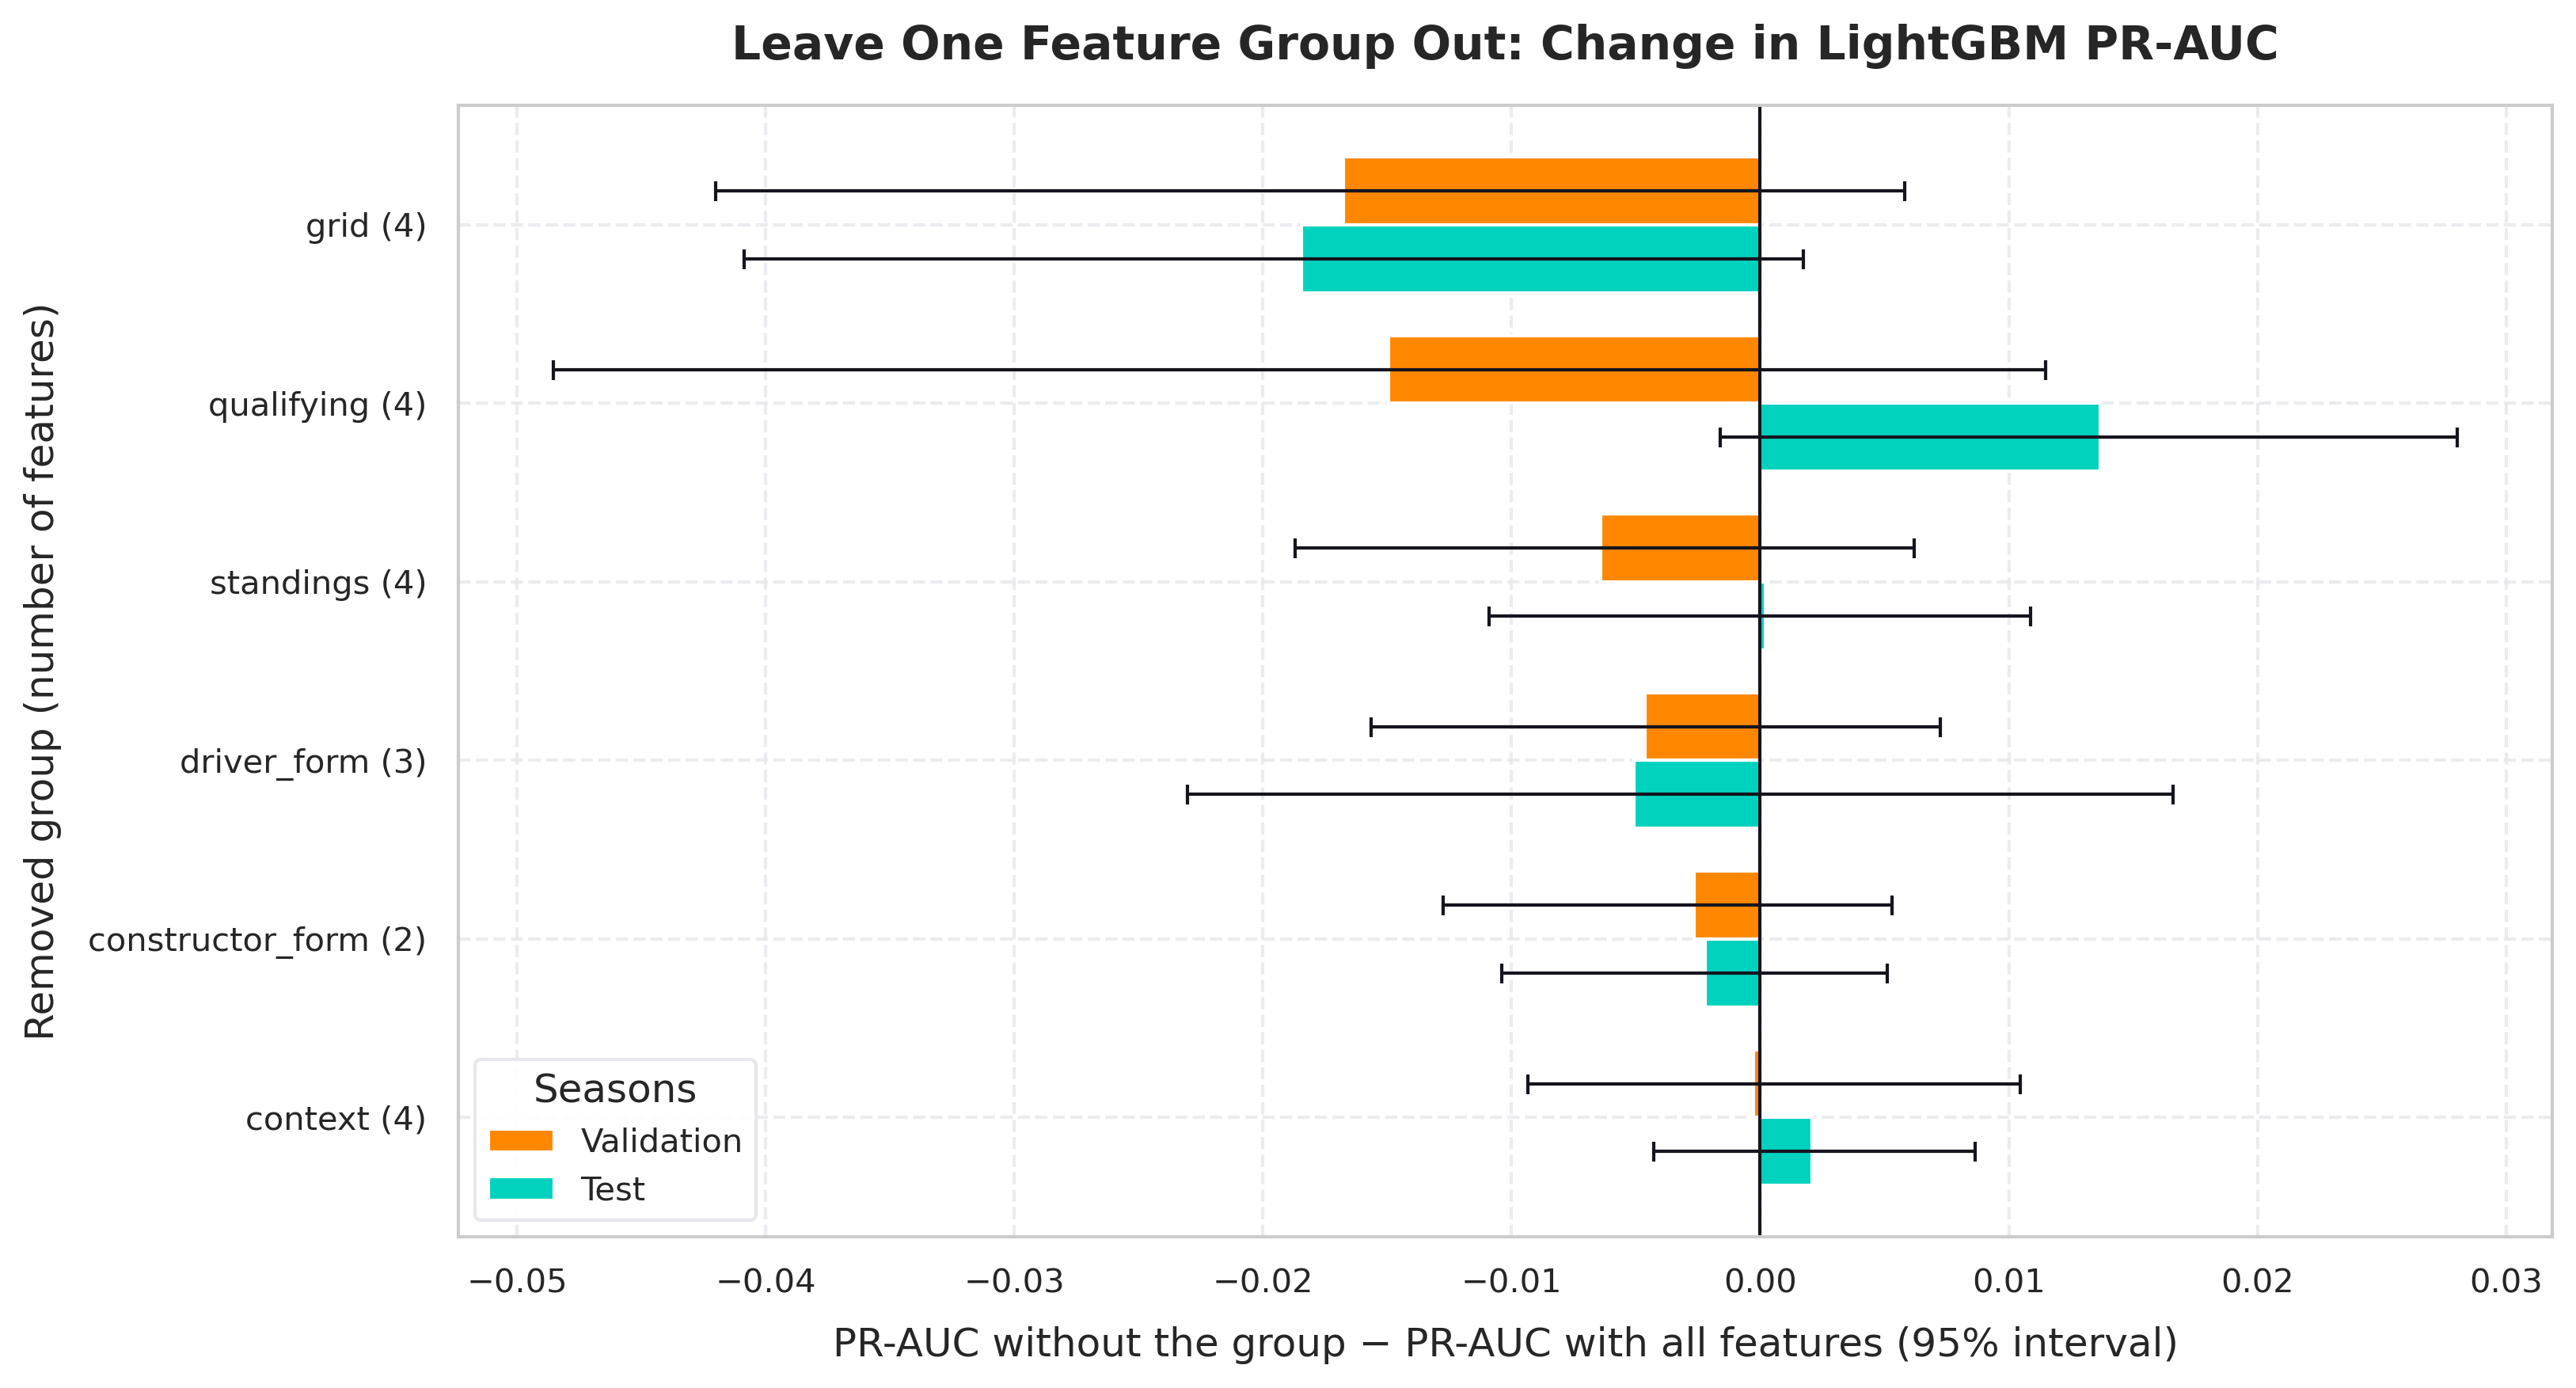
\includegraphics[width=\linewidth,height=0.42\textheight,keepaspectratio]{ablation_leave_one_group_out}
\caption{Change in PR-AUC when one feature group is removed, with 95\% intervals. Every interval crosses zero.}
\end{figure}

\begin{figure}[htbp]
\centering
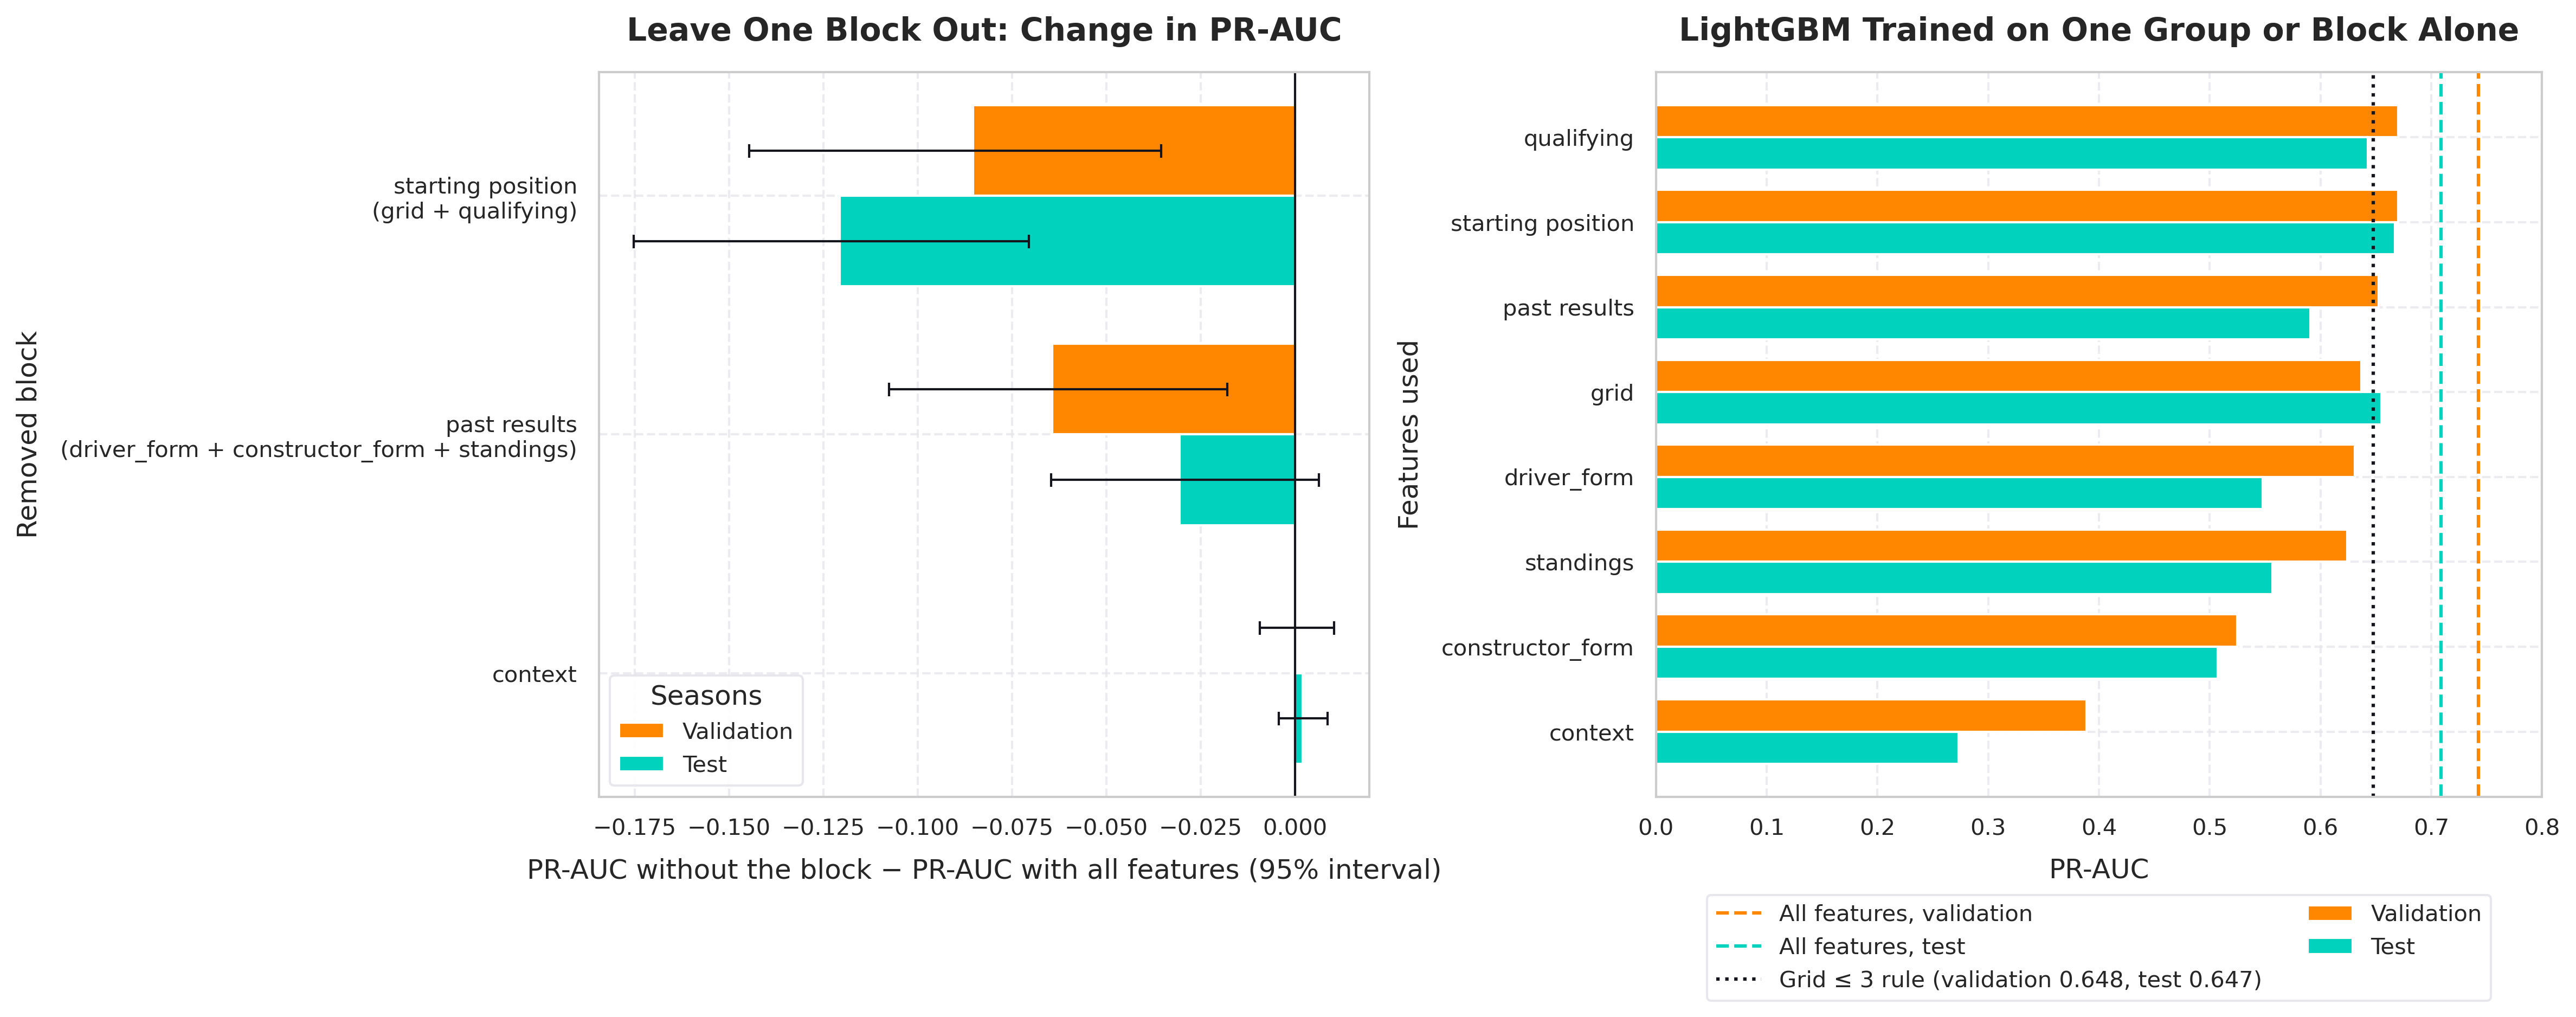
\includegraphics[width=\linewidth,height=0.42\textheight,keepaspectratio]{ablation_blocks_and_alone}
\caption{Left: change in PR-AUC when a block of overlapping groups is removed. Right: PR-AUC of a model trained on one group or block alone.}
\end{figure}

\section{Explainability}

All explanations are of the fitted LightGBM on the validation seasons (DEC-032). Nothing is retrained.

\subsection{Global: which features the model relies on}

\textbf{Permutation importance.} A feature is shuffled across the validation rows and the drop in PR-AUC is recorded (50 shuffles).

\begin{itemize}
\item \textbf{\texttt{grid} alone costs 0.229} (95\% range 0.148 to 0.302), about a third of the model's 0.743. No other single feature is clearly above zero.
\item \textbf{\texttt{quali\_\allowbreak{}position} costs 0.003}, although it is nearly the same number as \texttt{grid}: the model reads the starting position from \texttt{grid} and barely uses its copy.
\item \textbf{Single-feature importances do not add up.} They sum to 0.311, while shuffling everything at once costs 0.586. A feature that has a substitute is understated, so importance is reported per block as well.
\end{itemize}

\textbf{SHAP values.} For a tree model SHAP is exact: the base value plus the 21 contributions equals the model output for every row, which the notebook asserts. The unit is log-odds of the model score.

\begin{itemize}
\item \textbf{The starting-position block carries 54\% of all SHAP magnitude and past results 45\%.} Within the first block \texttt{grid} alone has 40\%, then come the team's recent points (12\%), the driver's career podium rate (8\%) and recent podium rate (8\%).
\item \textbf{The effect of \texttt{grid} is a staircase:} about +1.6 for slots 1 to 3, falling by 0.3 per slot to zero between slots 9 and 10, and about −1.0 for every slot from 15 back.
\item \textbf{Form features act as a switch:} a driver with at least one podium in the last five races gets about +0.2 to +0.3, one with none about −0.13, with little difference between one podium and five.
\item \textbf{Four features appear in no tree} (\texttt{pit\_\allowbreak{}start}, \texttt{missing\_\allowbreak{}quali\_\allowbreak{}flag}, \texttt{is\_\allowbreak{}home\_\allowbreak{}race}, \texttt{circuit\_\allowbreak{}historical\_\allowbreak{}podium\_\allowbreak{}rate}).
\end{itemize}

{\small
\begin{xltabular}{\linewidth}{>{\raggedright\arraybackslash}Xrrr}
\toprule
\textbf{Block} & \textbf{Share of SHAP magnitude} & \textbf{Permutation drop (fitted model)} & \textbf{Retraining drop (Section 7)} \\
\midrule
\endhead
Starting position & 54\% & 0.390 & 0.085 \\
Past results & 45\% & 0.167 & 0.064 \\
Context & 0.9\% & 0.000 & 0.000 \\
\bottomrule
\end{xltabular}
}

The three measures agree on the order and differ in size because they answer different questions. Permutation scrambles a block for the fitted model, which still trusts the scrambled values. Retraining lets a new model lean on what is left.

\textbf{Importance is quoted per block.} How the credit is split between \texttt{grid} and its near-copies (\texttt{quali\_\allowbreak{}position}, \texttt{gap\_\allowbreak{}to\_\allowbreak{}pole}) depends on the model's settings, not on the data: a LightGBM configuration that offers each tree half of the features moves \texttt{grid}'s share from about 42\% to about 28\%, while the starting-position block keeps about half of the total.

\begin{figure}[htbp]
\centering
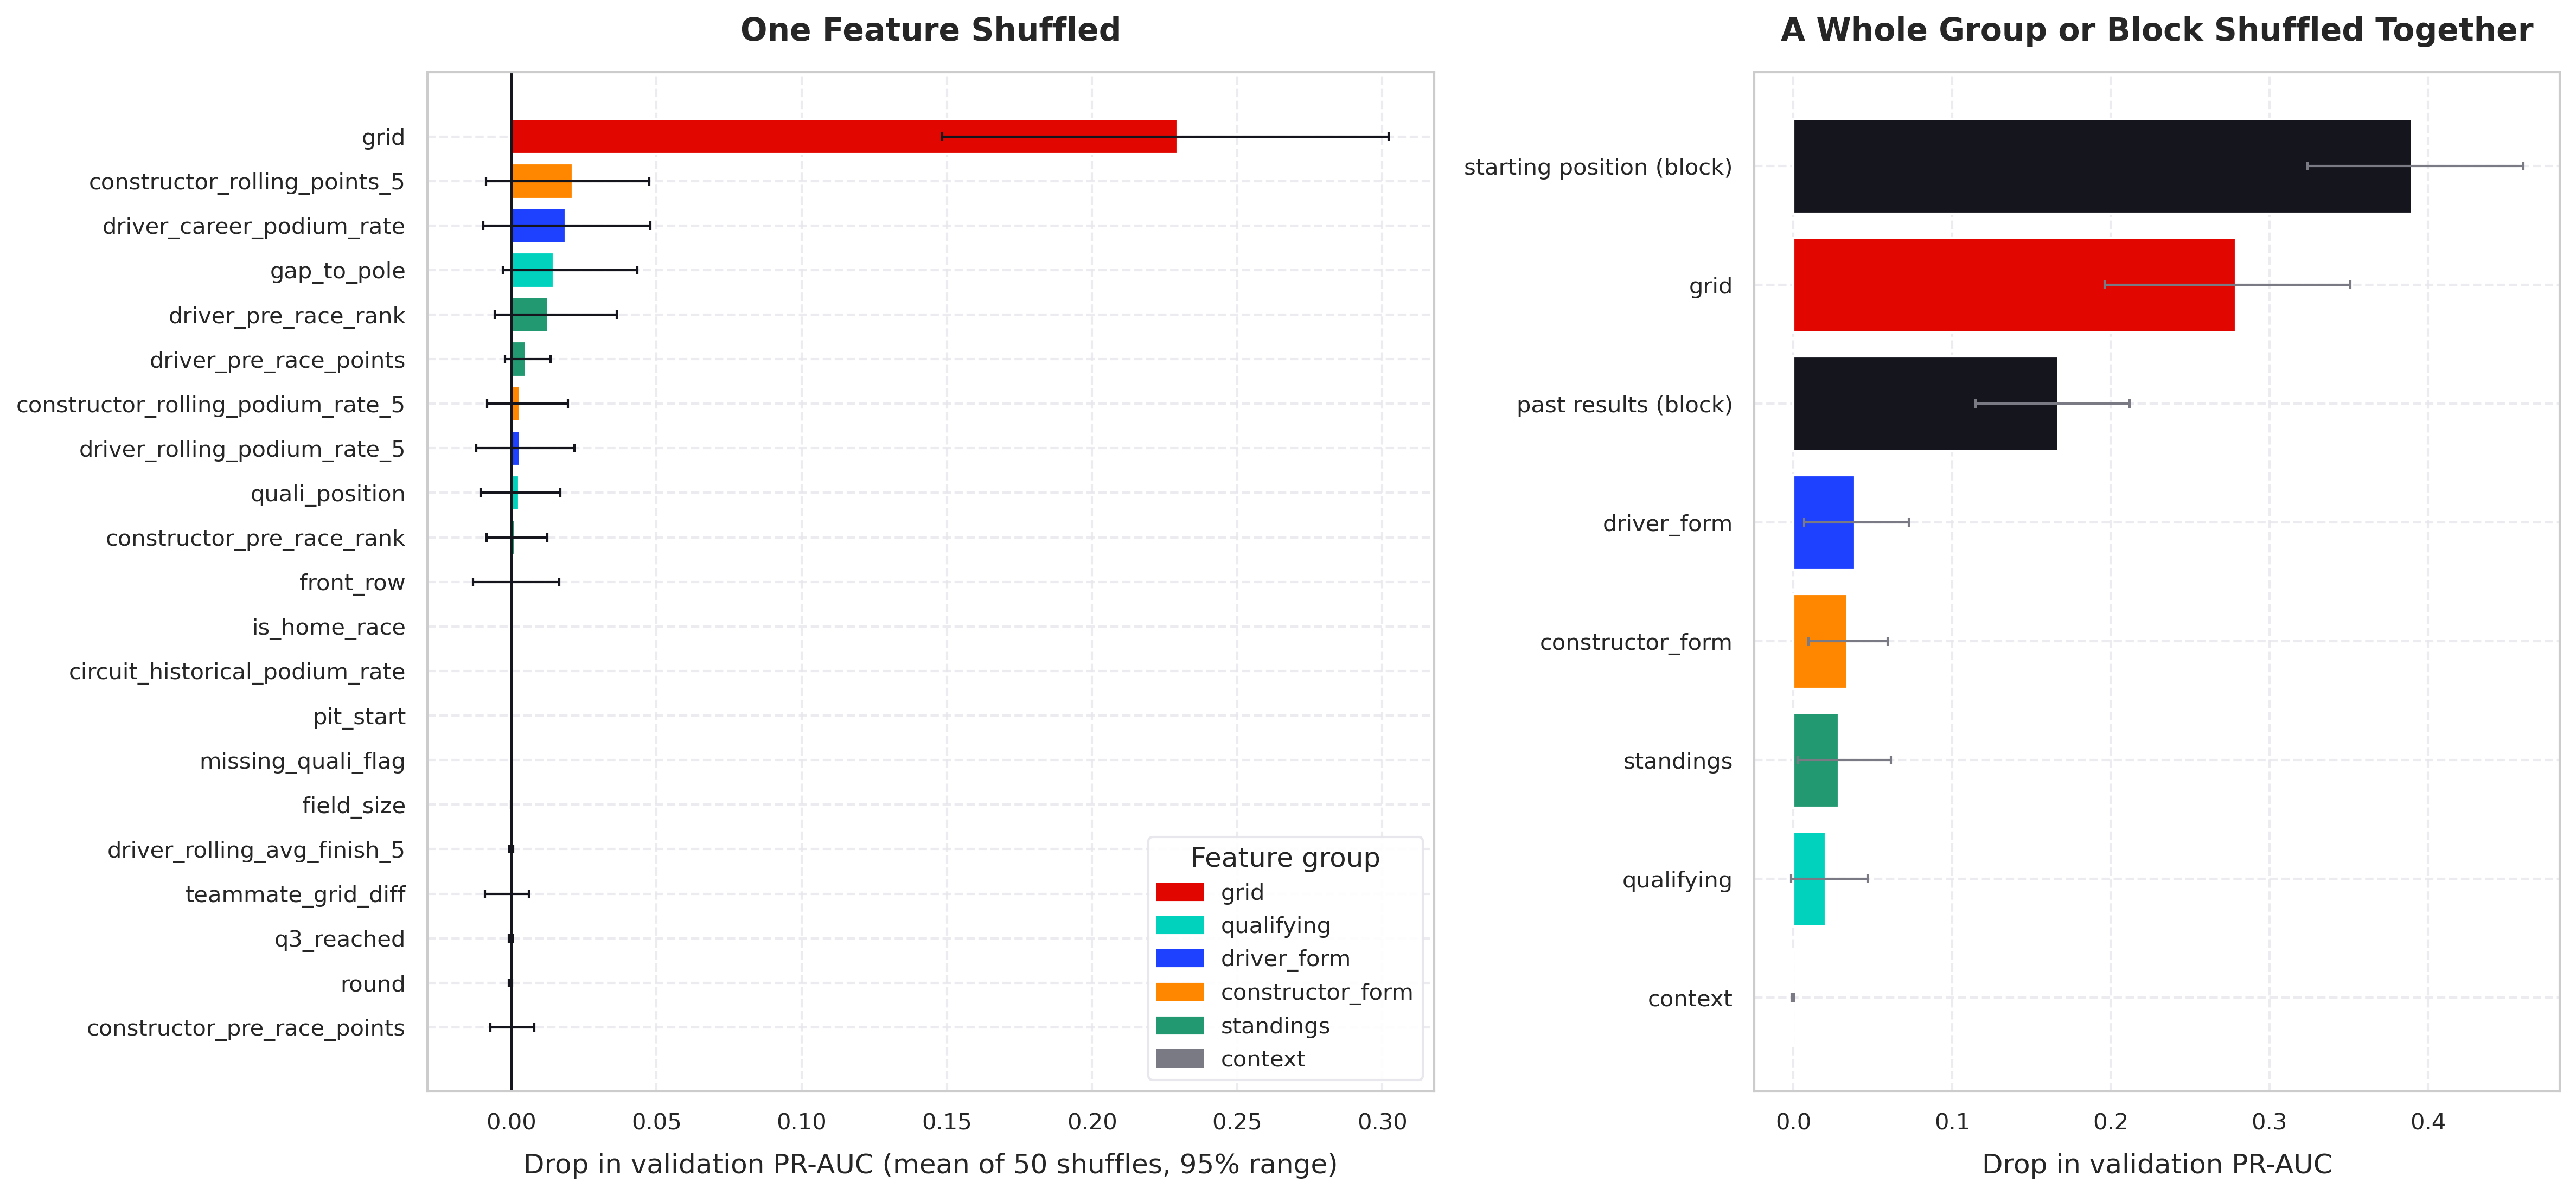
\includegraphics[width=\linewidth,height=0.42\textheight,keepaspectratio]{xai_permutation_importance}
\caption{Drop in validation PR-AUC when one feature is shuffled (left) and when a whole group or block is shuffled together (right).}
\end{figure}

\begin{figure}[htbp]
\centering
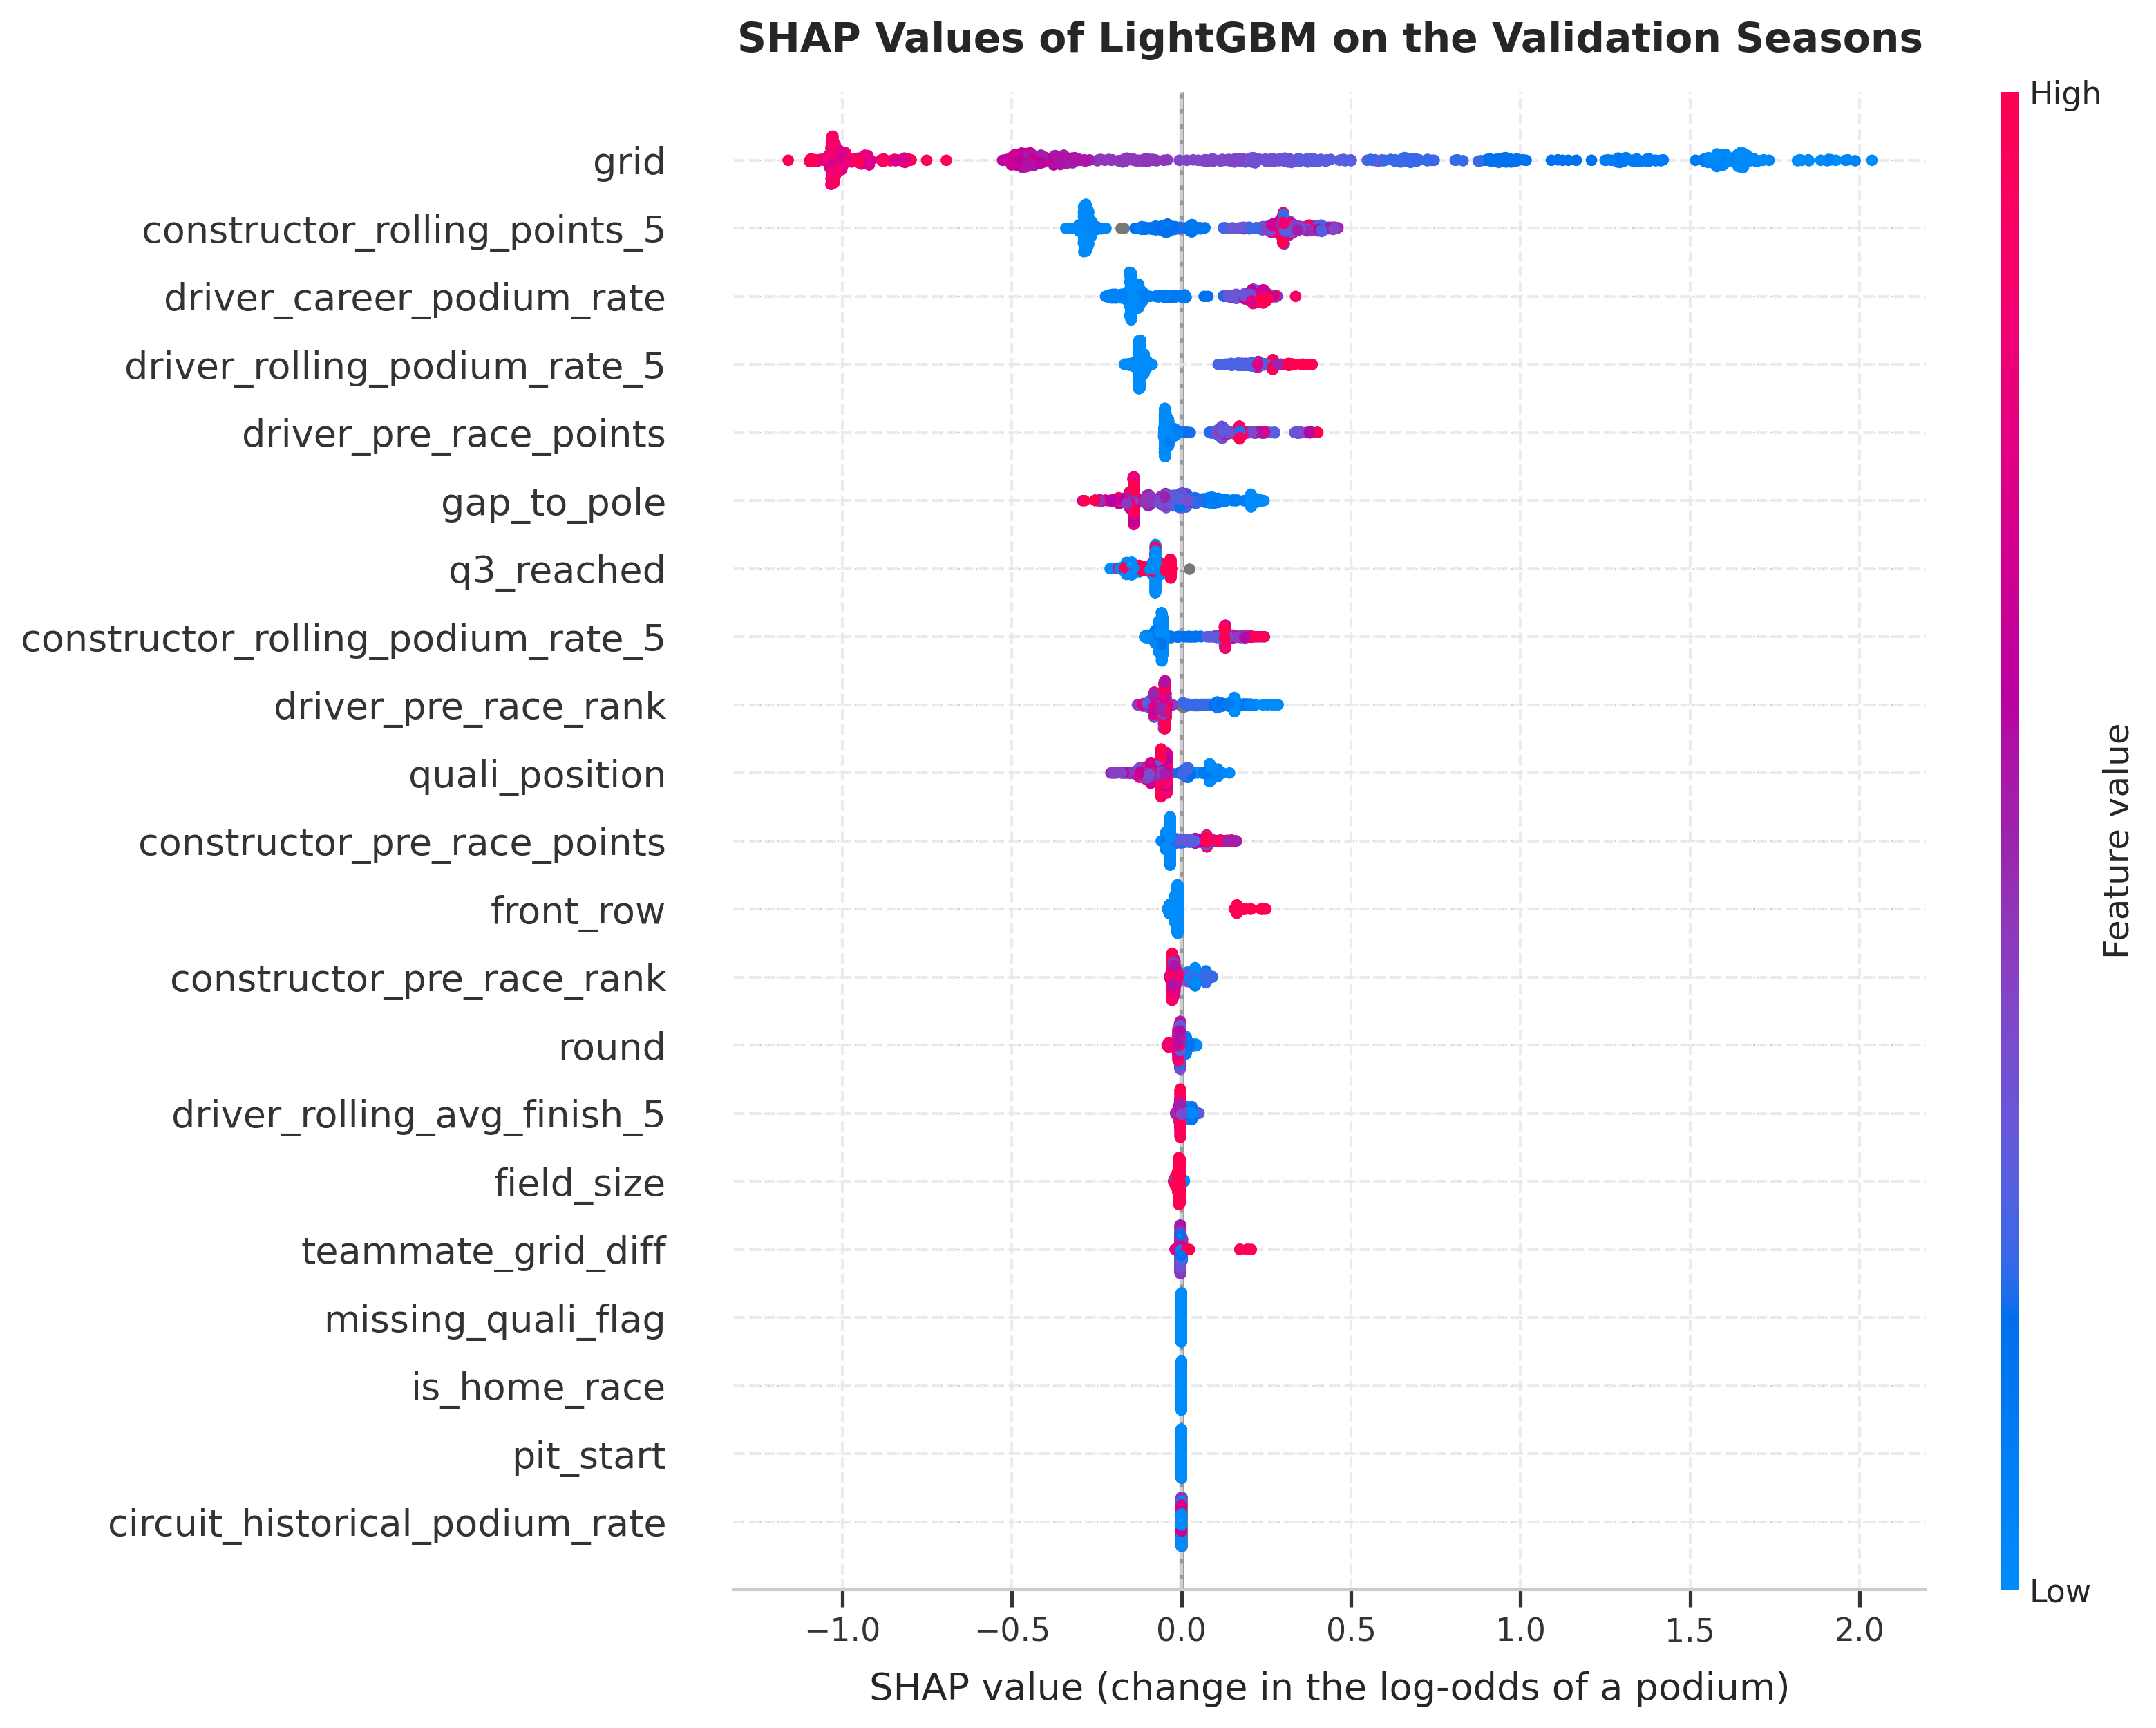
\includegraphics[width=\linewidth,height=0.42\textheight,keepaspectratio]{xai_shap_beeswarm}
\caption{SHAP summary (beeswarm) plot. One dot per validation row and feature; position is the contribution to the log-odds, colour is the feature value.}
\end{figure}

\subsection{Local: two surprising results}

Two validation rows were chosen by rule, not by hand: the podium finisher with the lowest score, and the pole-sitter off the podium with the highest score. Both come from the 2020 Italian Grand Prix.

{\small
\begin{xltabular}{\linewidth}{>{\raggedright\arraybackslash}Xr>{\raggedright\arraybackslash}X>{\raggedright\arraybackslash}X}
\toprule
\textbf{Case} & \textbf{Score} & \textbf{Result} & \textbf{Largest SHAP contributions (log-odds)} \\
\midrule
\endhead
Pierre Gasly (AlphaTauri), grid 10 & 0.127 & Won & Nearly all negative: career podium rate −0.13, no recent podium −0.12, \texttt{q3\_\allowbreak{}reached} −0.11, grid −0.11 \\
Lewis Hamilton (Mercedes), pole & 0.915 & Seventh & All positive: grid +1.65, team's recent points +0.30, five podiums in five races +0.27 \\
\bottomrule
\end{xltabular}
}

In both rows the model read its inputs sensibly. Nothing in Gasly's pre-race data suggested a podium, and everything in Hamilton's did. Both results were decided during the race, and that information does not exist before the start. Errors of this kind cannot be removed by tuning; they set a limit on any pre-race model.

\begin{figure}[htbp]
\centering
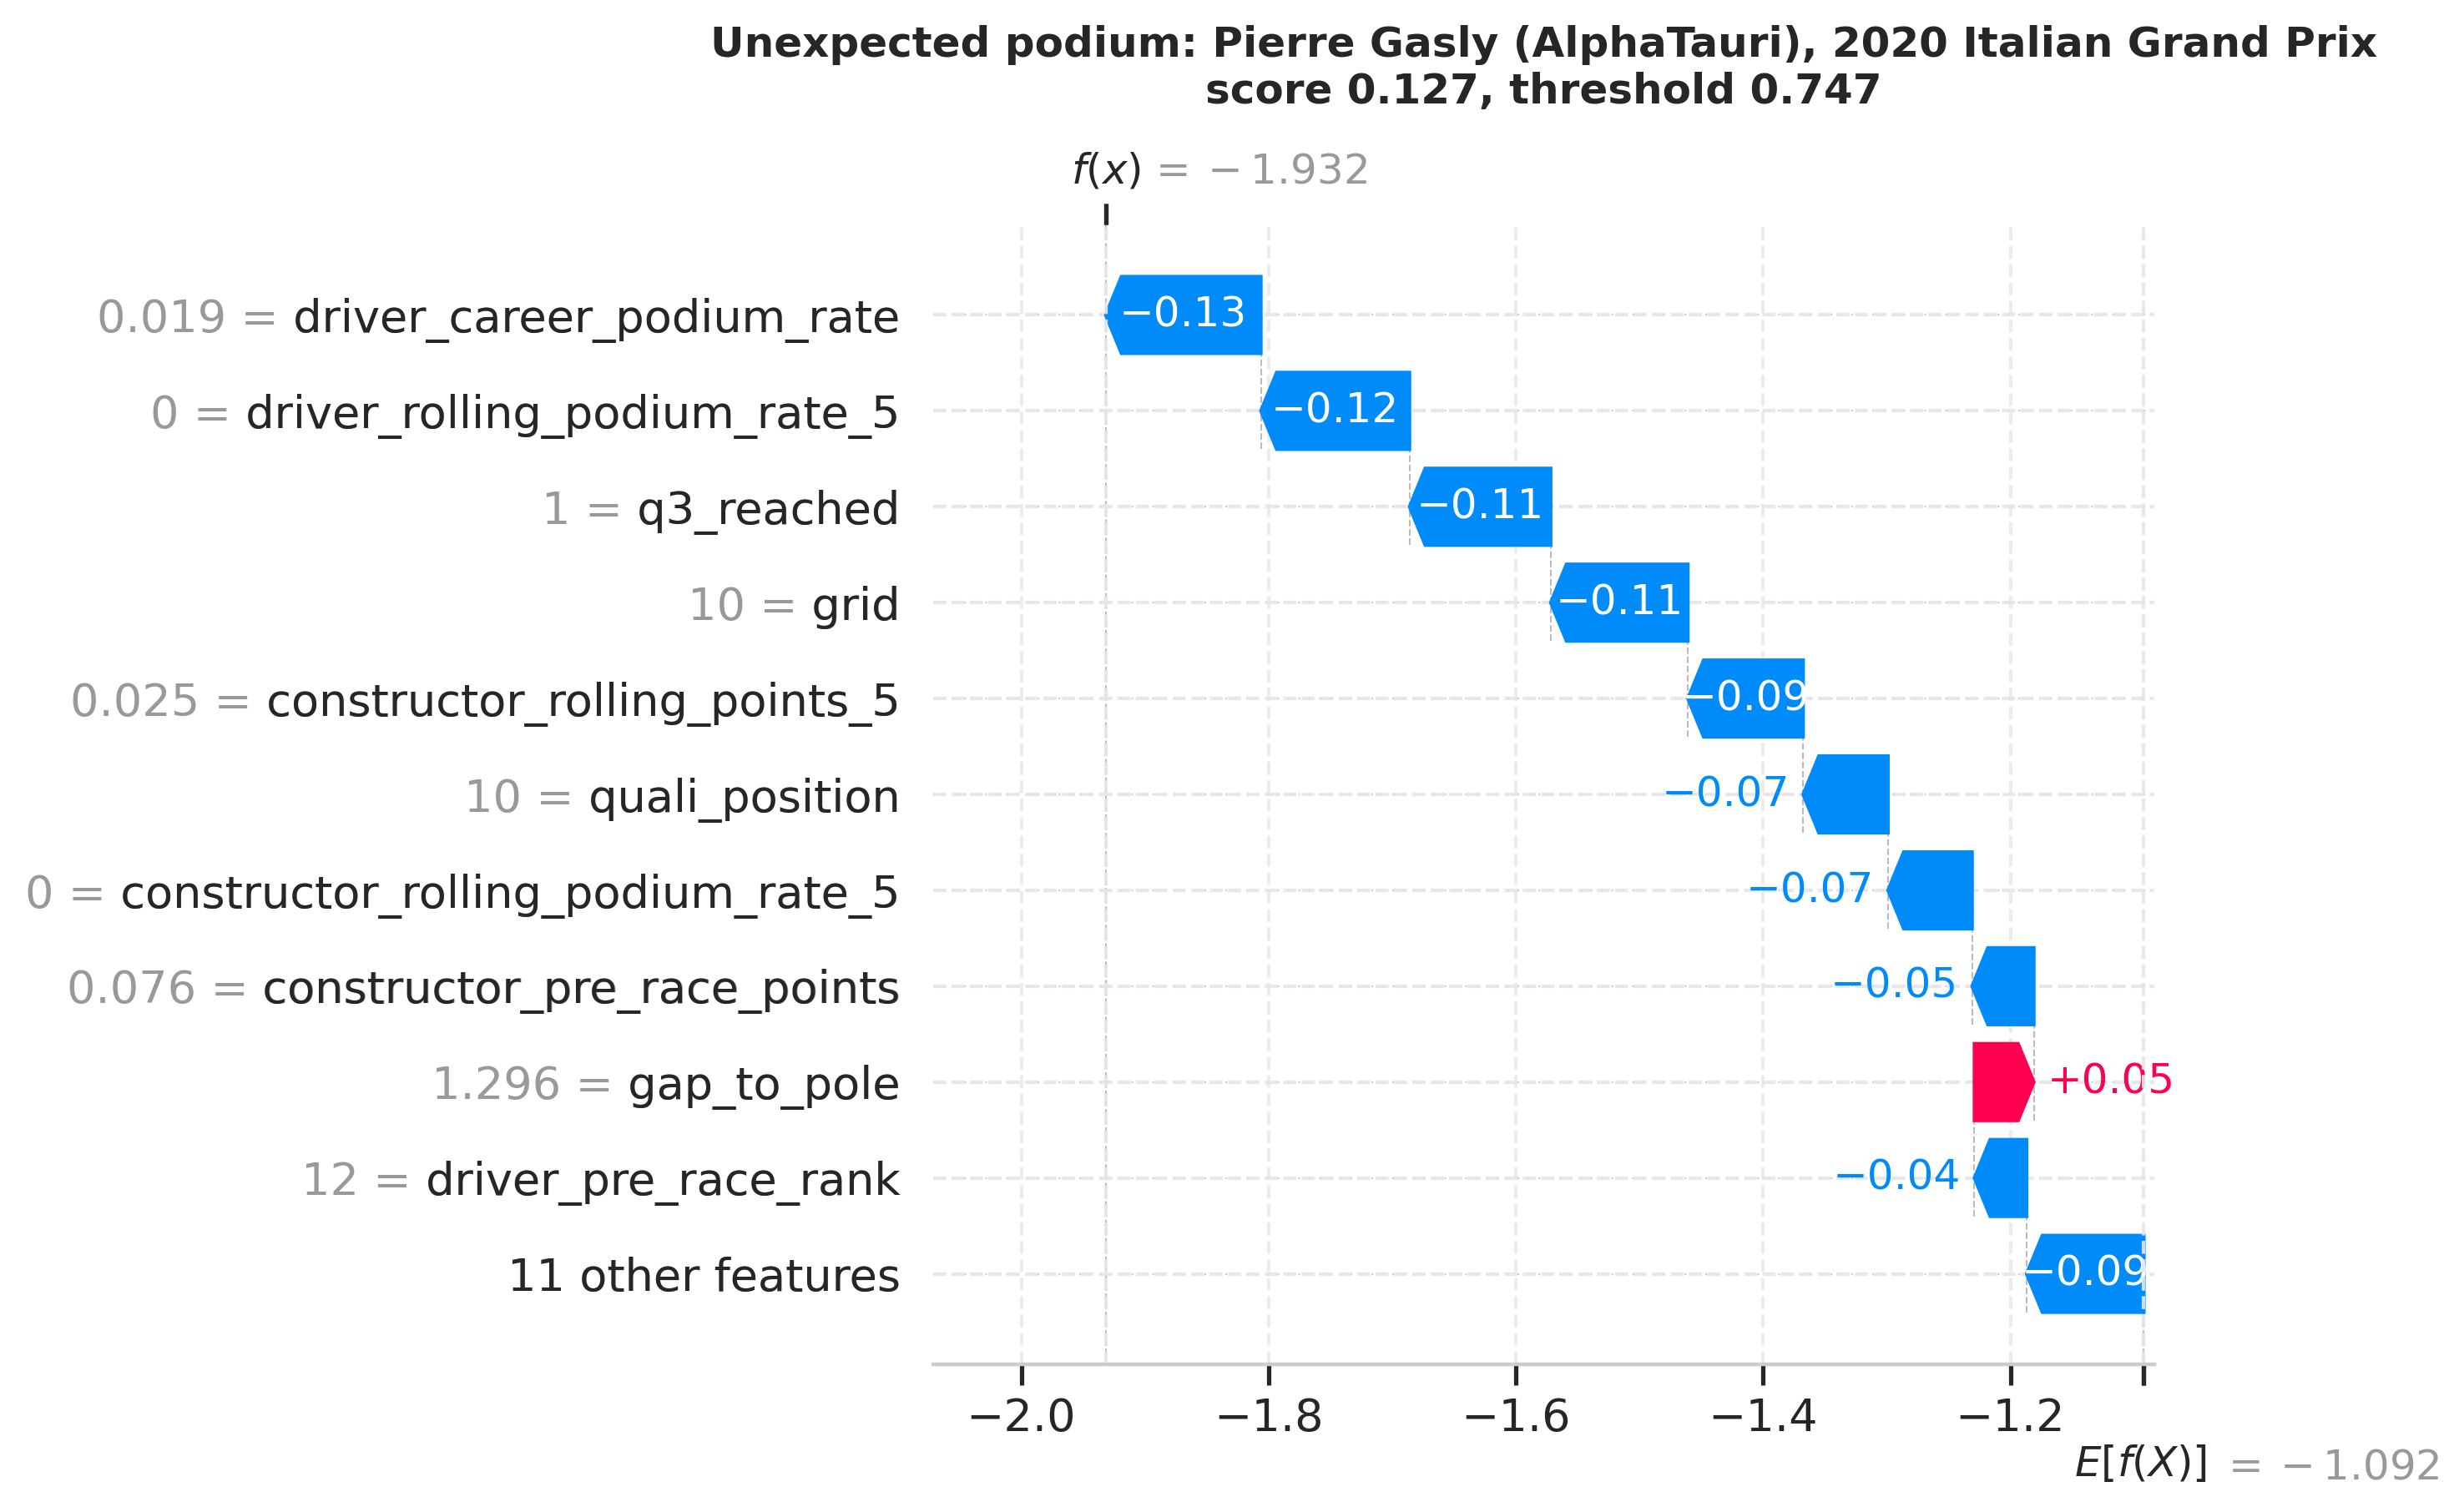
\includegraphics[width=\linewidth,height=0.42\textheight,keepaspectratio]{xai_shap_waterfall_unexpected_podium}
\caption{SHAP waterfall for Pierre Gasly, 2020 Italian Grand Prix. Read from the bottom: the plot starts at the base value and each bar adds one feature's contribution.}
\end{figure}

\begin{figure}[htbp]
\centering
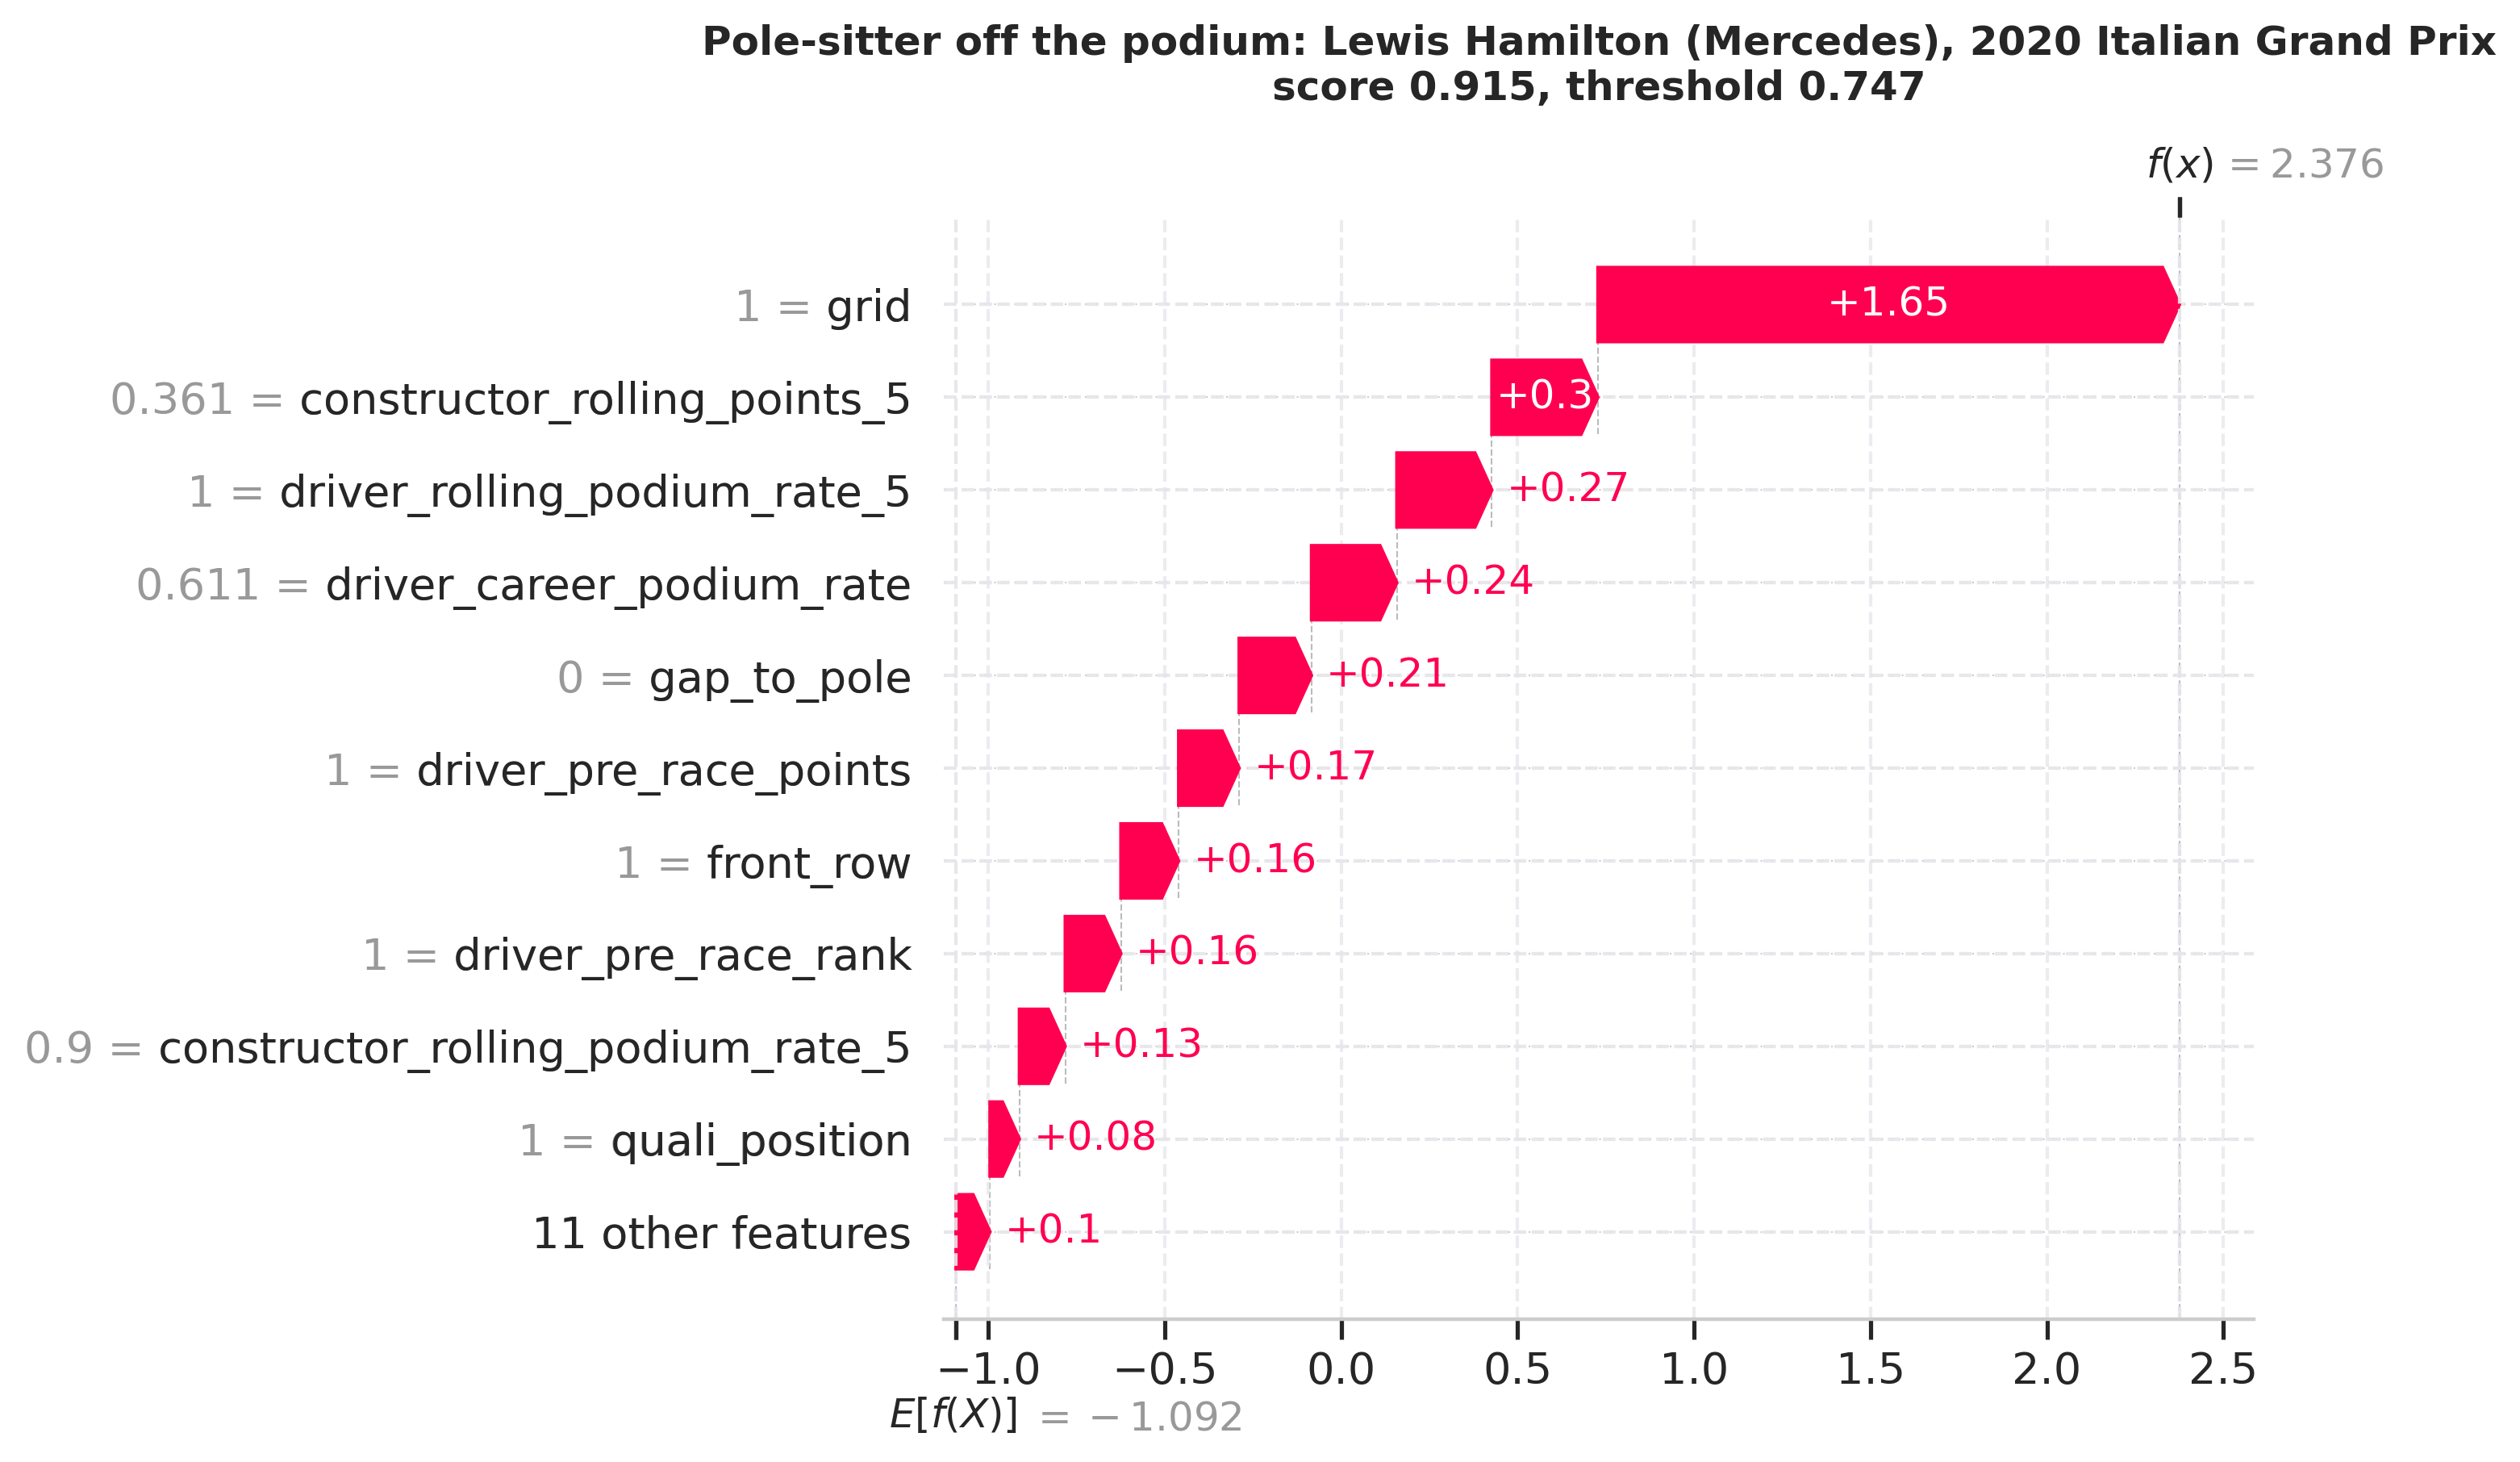
\includegraphics[width=\linewidth,height=0.42\textheight,keepaspectratio]{xai_shap_waterfall_pole_sitter_off_the_podium}
\caption{SHAP waterfall for Lewis Hamilton, 2020 Italian Grand Prix.}
\end{figure}

\textbf{LIME on the same two rows.} LIME fits a small linear model to the model's scores on 5,000 artificial rows around the row of interest.

{\small
\begin{xltabular}{\linewidth}{>{\raggedright\arraybackslash}Xrr}
\toprule
\textbf{} & \textbf{Gasly (score 0.127)} & \textbf{Hamilton (score 0.915)} \\
\midrule
\endhead
Fit of LIME's linear model (R²) & 0.05 & 0.82 \\
LIME's top feature & \texttt{pit\_\allowbreak{}start = 0} & \texttt{grid \textless{}= 5} \\
SHAP value of that feature & 0 (never used by the model) & +1.65 \\
Rank correlation with SHAP & 0.43 & 0.87 \\
Different top features across 5 random seeds & 3 & 1 \\
\bottomrule
\end{xltabular}
}

For Hamilton, LIME agrees with SHAP and is stable. For Gasly it fails: its linear model explains 5\% of the variation, and its top feature is one the model never uses. SHAP is therefore the primary method, and LIME is quoted only together with its R².

\subsection{What the explanations do not say}

\begin{itemize}
\item \textbf{Importance is not causation.} \texttt{grid} is important because it summarises how fast the car and driver are that weekend. Putting a slow car on pole would not make it a podium contender. The model has learned an association that holds when drivers reach their grid slot in the usual way.
\item \textbf{Credit between overlapping features is arbitrary.} \texttt{grid} and \texttt{quali\_\allowbreak{}position} are nearly the same number; the model happened to use \texttt{grid}. Importance should be quoted per block.
\item \textbf{A SHAP value can reflect how the data was recorded.} \texttt{q3\_\allowbreak{}reached} gets about −0.1 whether or not Q3 was reached, because only 25\% of training rows have a value for it.
\item \textbf{The explanations describe this model on 2020–2021}, in units of a class-weighted score, not of a calibrated probability.
\end{itemize}

\section{Inference Function}

\texttt{predict\_\allowbreak{}podium(raceId, driverId, grid, quali\_\allowbreak{}info=None)} returns a prediction (podium or not), a calibrated probability, the raw model score and the 21 features it built (DEC-033).

\begin{itemize}
\item \textbf{Features are rebuilt, not looked up.} The function runs the same feature code as training on the races before the requested one, plus that race's entry list with its results blanked. For 36 validation and test rows, including pit-lane starts, the rebuilt features and scores are identical to the modeling table.
\item \textbf{Missing values go to the model as missing.} LightGBM takes the raw features, so no value is invented for missing qualifying data. Most training seasons have no qualifying data, so the model has seen this in about 14,000 rows.
\item \textbf{The score is calibrated before it is called a probability.} Because of the class weights the raw score averages 0.32 where 15\% of rows are podiums. A one-input logistic regression fitted on validation (Platt scaling) corrects this without changing the order of the drivers. On the test seasons the mean probability is 0.161 against a podium rate of 0.151, and the Brier score falls from 0.117 to 0.069.
\end{itemize}

\textbf{Demonstration: the pole-sitter of the last race in the data} (Lando Norris, 2024 Abu Dhabi Grand Prix; he won).

{\small
\begin{xltabular}{\linewidth}{>{\raggedright\arraybackslash}Xrr>{\raggedright\arraybackslash}X}
\toprule
\textbf{Input} & \textbf{Score} & \textbf{Probability} & \textbf{Prediction} \\
\midrule
\endhead
Complete record & 0.901 & 0.756 & Podium \\
Qualifying position only, no lap times & 0.876 & 0.688 & Podium \\
No qualifying information & 0.866 & 0.663 & Podium \\
\bottomrule
\end{xltabular}
}

Across the whole 2024 season, removing qualifying from every row moves PR-AUC from 0.694 to 0.692, and 8 of 476 predictions change.

\begin{figure}[htbp]
\centering
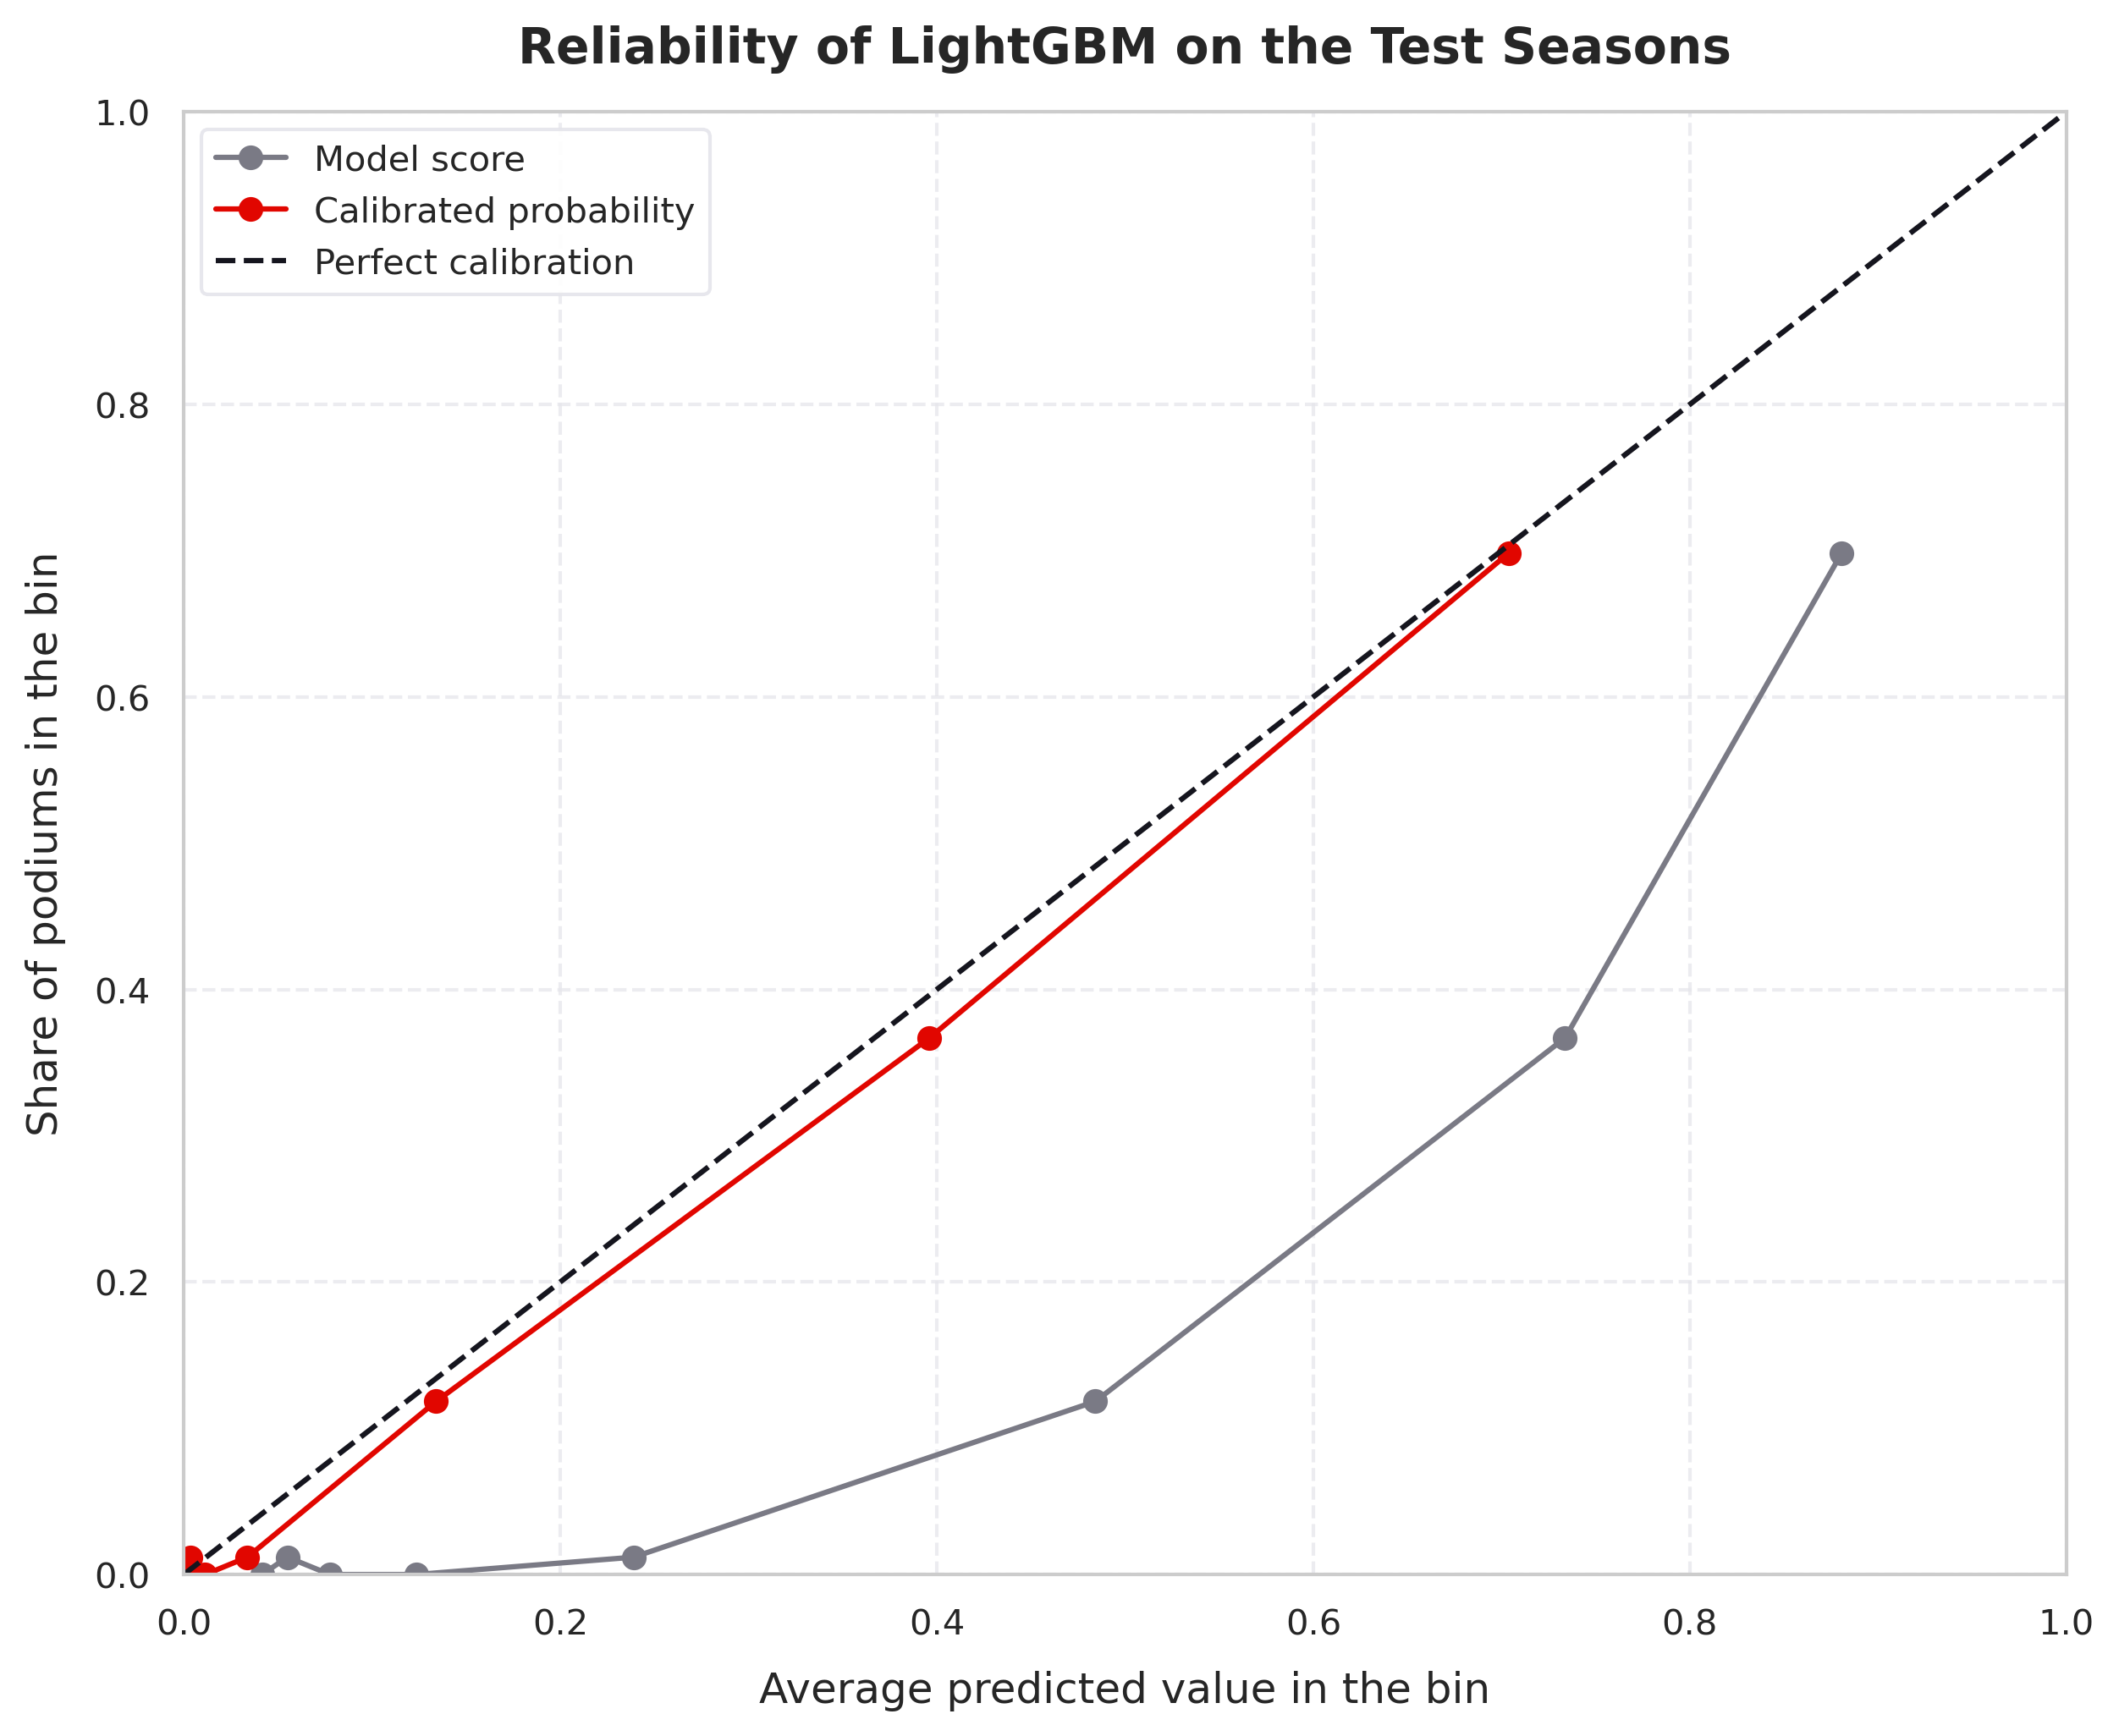
\includegraphics[width=\linewidth,height=0.42\textheight,keepaspectratio]{inference_calibration}
\caption{Share of podiums against the average predicted value, in eight equal groups of test rows. Points on the diagonal are perfectly calibrated.}
\end{figure}

\section{Limitations and Future Work}

\textbf{Data}

\begin{itemize}
\item \textbf{Historical qualifying drift.} The four qualifying features are missing in 63\% of the training rows and in almost none of the validation and test rows. The model learns the value of qualifying from about a third of its training data.
\item \textbf{The training seasons are unlike the test seasons.} Training runs from 1950: larger and more variable fields, a lower podium rate, different points systems.
\item \textbf{Era boundaries are not modelled.} Regulation changes (2014, 2022) reshuffle which teams are fast, and the model sees them only through form and standings, which lag by a few races. Features built from past results transfer less well to 2022–2024 than the starting position does.
\item \textbf{Constructor identity breaks at rebrands.} A renamed team starts its rolling history from nothing. The lineage mapping built for Q3 was not used for the features.
\item \textbf{Shared drives are removed, not resolved.} The data cannot say which driver started a shared car, so 157 rows of 1950–1964 are dropped (0.7\% of the training rows) and 15 early races keep fewer than three podium rows.
\end{itemize}

\textbf{Evaluation}

\begin{itemize}
\item \textbf{Small validation and test sets.} 39 and 68 races. Intervals on PR-AUC differences are about ±0.02 to ±0.03, so the learned models cannot be separated.
\item \textbf{The thresholds do not transfer well} from validation to test.
\item \textbf{Tuning is sensitive to small changes in the data.} With one seed per configuration, a 0.4\% change in the training rows changed every search's winner. Seed-averaged tuning (DEC-037) fixes the selection, at five times the cost.
\item \textbf{The test seasons have been used.} One model comparison was made on them and nothing was chosen from it. They were scored again to describe the features (Section 7) and to check the calibration (Section 9). They are no longer untouched data for any future change.
\end{itemize}

\textbf{Model}

\begin{itemize}
\item \textbf{In-race events set a ceiling.} Crashes, safety cars, penalties, weather and strategy are not in the inputs.
\item \textbf{Four of the 21 features are never used}, and the context group contributes nothing.
\item \textbf{The output is unreliable for unusual inputs.} For a front-running car starting last, the function's output rises, which the training data does not support.
\item \textbf{The inference function works only for races in the dataset}, whose history ends with the 2024 season.
\end{itemize}

\textbf{Future work}

\begin{itemize}
\item Use the lineage of renamed teams in the features.
\item Drop the unused features and compare a logistic regression with LightGBM on a new, untouched season.
\item Rank drivers within a race instead of scoring rows independently, since every race has exactly three podium places.
\item Add pre-race information the dataset does not hold: practice pace, weather forecast, tyre allocation.
\item Tune with several consecutive validation windows instead of one 39-race window.
\end{itemize}

\end{document}
